
\section{Robustness of Implementation}
\subsection{Bus hangup}

\subsection{i2c errors per time}

\subsection{Integration Test for Quadcopter}


\section{Ranging Accuracy}

\subsection{Influence of DQF on Range Values}
One value the ranging api provides is the DQF\footnote{Data Quality Factor}-value.
It is reasonable to expect a huge amount of scatter for lower DQF values.
As \autoref{1m_scatterplot} shows this is not how the range value behaves.

For the values measured with 1m real distance we can see that the values measered with lower quality do not have the same mean value as those with higher quality.
Also values measured with lower quality are closer to each other than those with higher signal quality.
As long as we only look at the values taken at 1m real distance it seams like we could be able to improve the range estimate by including the dqf value into the computation of the distance.
To do that this behaviour would need to be stable accross different distances, i.e. no matter if the measurement is taken at 1m or 3m distance the when the dqf is low the measured range is lower and if dqf is high the measured range is higher.
\begin{figure}[H]
	\centering
	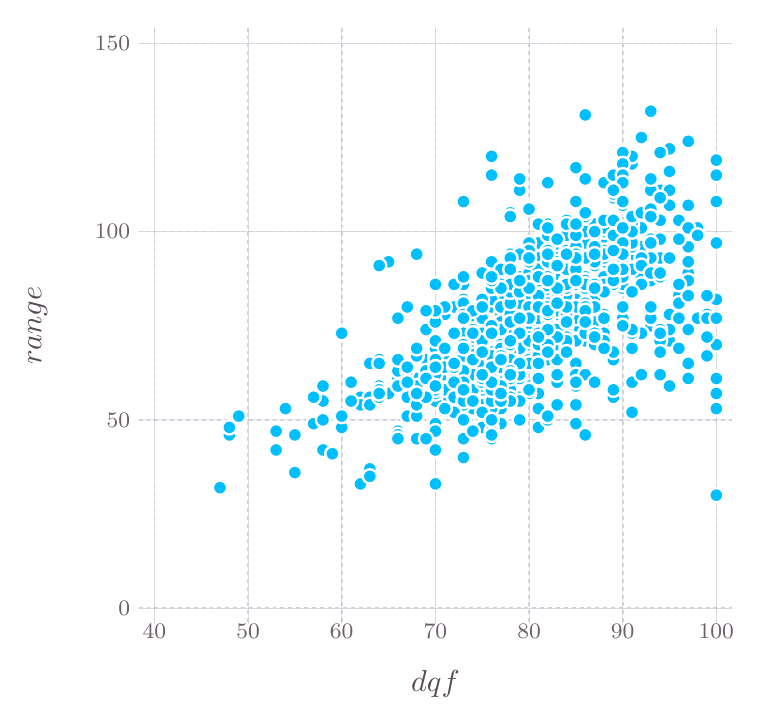
\begin{tikzpicture}[x=1mm,y=-1mm]
\definecolor{mycolor00BFFF}{rgb}{0,0.75,1}
\definecolor{mycolor564A55}{rgb}{0.34,0.29,0.33}
\definecolor{mycolor000000}{rgb}{0,0,0}
\definecolor{mycolor6C606B}{rgb}{0.42,0.38,0.42}
\definecolor{mycolorD0D0E0}{rgb}{0.82,0.82,0.88}
\definecolor{mycolorFFFFFF}{rgb}{1,1,1}
\definecolor{mycolor000000}{rgb}{0,0,0}
\begin{scope}
\begin{scope}
\draw (57.32,88.39) node [text=mycolor564A55,draw=mycolor000000,draw opacity=0,rotate around={-0: (0,1.81)},inner sep=0.0]{\fontsize{3.88mm}{4.66mm}\selectfont $\text{dqf}$};
\end{scope}
\begin{scope}
\draw (21.63,81.72) node [text=mycolor6C606B,rotate around={-0: (35.68,1.34)},inner sep=0.0]{\fontsize{2.82mm}{3.39mm}\selectfont $\text{40}$};
\draw (33.53,81.72) node [text=mycolor6C606B,rotate around={-0: (23.79,1.34)},inner sep=0.0]{\fontsize{2.82mm}{3.39mm}\selectfont $\text{50}$};
\draw (45.42,81.72) node [text=mycolor6C606B,rotate around={-0: (11.89,1.34)},inner sep=0.0]{\fontsize{2.82mm}{3.39mm}\selectfont $\text{60}$};
\draw (57.32,81.72) node [text=mycolor6C606B,rotate around={-0: (-0,1.34)},inner sep=0.0]{\fontsize{2.82mm}{3.39mm}\selectfont $\text{70}$};
\draw (69.21,81.72) node [text=mycolor6C606B,rotate around={-0: (-11.89,1.34)},inner sep=0.0]{\fontsize{2.82mm}{3.39mm}\selectfont $\text{80}$};
\draw (81.11,81.72) node [text=mycolor6C606B,rotate around={-0: (-23.79,1.34)},inner sep=0.0]{\fontsize{2.82mm}{3.39mm}\selectfont $\text{90}$};
\draw (93,81.72) node [text=mycolor6C606B,rotate around={-0: (-35.68,1.34)},inner sep=0.0]{\fontsize{2.82mm}{3.39mm}\selectfont $\text{100}$};
\end{scope}
\begin{scope}
\clip  (19.63,5) -- (95,5) -- (95,80.72) -- (19.63,80.72);
\begin{scope}
\clip  (19.63,5) -- (95,5) -- (95,80.72) -- (19.63,80.72);
\path [fill=mycolor000000,fill opacity=0,draw=mycolor000000,draw opacity=0] (19.63,5) rectangle +(75.37,75.72);
\end{scope}
\begin{scope}
[dash pattern=on 0.5mm off 0.5mm,line width=0.2mm]
\path [fill=mycolor000000,draw=mycolorD0D0E0]  (19.63,78.71) -- (95,78.71);
\path [fill=mycolor000000,draw=mycolorD0D0E0]  (19.63,54.81) -- (95,54.81);
\path [fill=mycolor000000,draw=mycolorD0D0E0]  (19.63,30.9) -- (95,30.9);
\path [fill=mycolor000000,draw=mycolorD0D0E0]  (19.63,7) -- (95,7);
\end{scope}
\begin{scope}
[dash pattern=on 0.5mm off 0.5mm,line width=0.2mm]
\path [fill=mycolor000000,draw=mycolorD0D0E0]  (21.63,5) -- (21.63,80.72);
\path [fill=mycolor000000,draw=mycolorD0D0E0]  (33.53,5) -- (33.53,80.72);
\path [fill=mycolor000000,draw=mycolorD0D0E0]  (45.42,5) -- (45.42,80.72);
\path [fill=mycolor000000,draw=mycolorD0D0E0]  (57.32,5) -- (57.32,80.72);
\path [fill=mycolor000000,draw=mycolorD0D0E0]  (69.21,5) -- (69.21,80.72);
\path [fill=mycolor000000,draw=mycolorD0D0E0]  (81.11,5) -- (81.11,80.72);
\path [fill=mycolor000000,draw=mycolorD0D0E0]  (93,5) -- (93,80.72);
\end{scope}
\begin{scope}
\begin{scope}
\begin{scope}
[line width=0.3mm]
\path [fill=mycolor00BFFF,draw=mycolorFFFFFF] (66.83,28.51) circle [radius=0.9];
\path [fill=mycolor00BFFF,draw=mycolorFFFFFF] (84.67,42.86) circle [radius=0.9];
\path [fill=mycolor00BFFF,draw=mycolorFFFFFF] (50.18,47.16) circle [radius=0.9];
\path [fill=mycolor00BFFF,draw=mycolorFFFFFF] (88.24,39.03) circle [radius=0.9];
\path [fill=mycolor00BFFF,draw=mycolorFFFFFF] (87.05,43.34) circle [radius=0.9];
\path [fill=mycolor00BFFF,draw=mycolorFFFFFF] (57.32,56.24) circle [radius=0.9];
\path [fill=mycolor00BFFF,draw=mycolorFFFFFF] (71.59,40.95) circle [radius=0.9];
\path [fill=mycolor00BFFF,draw=mycolorFFFFFF] (78.73,38.55) circle [radius=0.9];
\path [fill=mycolor00BFFF,draw=mycolorFFFFFF] (72.78,41.42) circle [radius=0.9];
\path [fill=mycolor00BFFF,draw=mycolorFFFFFF] (69.21,43.81) circle [radius=0.9];
\path [fill=mycolor00BFFF,draw=mycolorFFFFFF] (73.97,39.03) circle [radius=0.9];
\path [fill=mycolor00BFFF,draw=mycolorFFFFFF] (77.54,41.9) circle [radius=0.9];
\path [fill=mycolor00BFFF,draw=mycolorFFFFFF] (52.56,49.07) circle [radius=0.9];
\path [fill=mycolor00BFFF,draw=mycolorFFFFFF] (76.35,36.64) circle [radius=0.9];
\path [fill=mycolor00BFFF,draw=mycolorFFFFFF] (63.26,51.46) circle [radius=0.9];
\path [fill=mycolor00BFFF,draw=mycolorFFFFFF] (62.07,46.68) circle [radius=0.9];
\path [fill=mycolor00BFFF,draw=mycolorFFFFFF] (70.4,45.25) circle [radius=0.9];
\path [fill=mycolor00BFFF,draw=mycolorFFFFFF] (60.88,50.99) circle [radius=0.9];
\path [fill=mycolor00BFFF,draw=mycolorFFFFFF] (66.83,47.16) circle [radius=0.9];
\path [fill=mycolor00BFFF,draw=mycolorFFFFFF] (76.35,44.77) circle [radius=0.9];
\path [fill=mycolor00BFFF,draw=mycolorFFFFFF] (87.05,44.77) circle [radius=0.9];
\path [fill=mycolor00BFFF,draw=mycolorFFFFFF] (58.51,52.42) circle [radius=0.9];
\path [fill=mycolor00BFFF,draw=mycolorFFFFFF] (63.26,50.51) circle [radius=0.9];
\path [fill=mycolor00BFFF,draw=mycolorFFFFFF] (87.05,43.34) circle [radius=0.9];
\path [fill=mycolor00BFFF,draw=mycolorFFFFFF] (66.83,46.68) circle [radius=0.9];
\path [fill=mycolor00BFFF,draw=mycolorFFFFFF] (93,32.34) circle [radius=0.9];
\path [fill=mycolor00BFFF,draw=mycolorFFFFFF] (57.32,55.29) circle [radius=0.9];
\path [fill=mycolor00BFFF,draw=mycolorFFFFFF] (64.45,57.2) circle [radius=0.9];
\path [fill=mycolor00BFFF,draw=mycolorFFFFFF] (78.73,42.38) circle [radius=0.9];
\path [fill=mycolor00BFFF,draw=mycolorFFFFFF] (87.05,27.56) circle [radius=0.9];
\path [fill=mycolor00BFFF,draw=mycolorFFFFFF] (82.29,22.3) circle [radius=0.9];
\path [fill=mycolor00BFFF,draw=mycolorFFFFFF] (82.29,34.25) circle [radius=0.9];
\path [fill=mycolor00BFFF,draw=mycolorFFFFFF] (71.59,39.03) circle [radius=0.9];
\path [fill=mycolor00BFFF,draw=mycolorFFFFFF] (64.45,38.08) circle [radius=0.9];
\path [fill=mycolor00BFFF,draw=mycolorFFFFFF] (78.73,31.86) circle [radius=0.9];
\path [fill=mycolor00BFFF,draw=mycolorFFFFFF] (60.88,49.55) circle [radius=0.9];
\path [fill=mycolor00BFFF,draw=mycolorFFFFFF] (71.59,35.69) circle [radius=0.9];
\path [fill=mycolor00BFFF,draw=mycolorFFFFFF] (89.43,43.34) circle [radius=0.9];
\path [fill=mycolor00BFFF,draw=mycolorFFFFFF] (63.26,52.42) circle [radius=0.9];
\path [fill=mycolor00BFFF,draw=mycolorFFFFFF] (91.81,46.68) circle [radius=0.9];
\path [fill=mycolor00BFFF,draw=mycolorFFFFFF] (75.16,42.86) circle [radius=0.9];
\path [fill=mycolor00BFFF,draw=mycolorFFFFFF] (70.4,39.51) circle [radius=0.9];
\path [fill=mycolor00BFFF,draw=mycolorFFFFFF] (76.35,33.77) circle [radius=0.9];
\path [fill=mycolor00BFFF,draw=mycolorFFFFFF] (66.83,49.07) circle [radius=0.9];
\path [fill=mycolor00BFFF,draw=mycolorFFFFFF] (53.75,50.99) circle [radius=0.9];
\path [fill=mycolor00BFFF,draw=mycolorFFFFFF] (93,64.37) circle [radius=0.9];
\path [fill=mycolor00BFFF,draw=mycolorFFFFFF] (66.83,33.77) circle [radius=0.9];
\path [fill=mycolor00BFFF,draw=mycolorFFFFFF] (68.02,51.94) circle [radius=0.9];
\path [fill=mycolor00BFFF,draw=mycolorFFFFFF] (69.21,47.64) circle [radius=0.9];
\path [fill=mycolor00BFFF,draw=mycolorFFFFFF] (39.47,61.5) circle [radius=0.9];
\path [fill=mycolor00BFFF,draw=mycolorFFFFFF] (54.94,57.2) circle [radius=0.9];
\path [fill=mycolor00BFFF,draw=mycolorFFFFFF] (69.21,50.51) circle [radius=0.9];
\path [fill=mycolor00BFFF,draw=mycolorFFFFFF] (43.04,58.63) circle [radius=0.9];
\path [fill=mycolor00BFFF,draw=mycolorFFFFFF] (83.48,43.81) circle [radius=0.9];
\path [fill=mycolor00BFFF,draw=mycolorFFFFFF] (68.02,41.9) circle [radius=0.9];
\path [fill=mycolor00BFFF,draw=mycolorFFFFFF] (73.97,44.77) circle [radius=0.9];
\path [fill=mycolor00BFFF,draw=mycolorFFFFFF] (93,53.38) circle [radius=0.9];
\path [fill=mycolor00BFFF,draw=mycolorFFFFFF] (59.69,53.85) circle [radius=0.9];
\path [fill=mycolor00BFFF,draw=mycolorFFFFFF] (72.78,34.25) circle [radius=0.9];
\path [fill=mycolor00BFFF,draw=mycolorFFFFFF] (68.02,25.65) circle [radius=0.9];
\path [fill=mycolor00BFFF,draw=mycolorFFFFFF] (71.59,39.99) circle [radius=0.9];
\path [fill=mycolor00BFFF,draw=mycolorFFFFFF] (79.92,32.82) circle [radius=0.9];
\path [fill=mycolor00BFFF,draw=mycolorFFFFFF] (69.21,33.3) circle [radius=0.9];
\path [fill=mycolor00BFFF,draw=mycolorFFFFFF] (82.29,34.25) circle [radius=0.9];
\path [fill=mycolor00BFFF,draw=mycolorFFFFFF] (79.92,36.16) circle [radius=0.9];
\path [fill=mycolor00BFFF,draw=mycolorFFFFFF] (75.16,36.64) circle [radius=0.9];
\path [fill=mycolor00BFFF,draw=mycolorFFFFFF] (60.88,43.34) circle [radius=0.9];
\path [fill=mycolor00BFFF,draw=mycolorFFFFFF] (58.51,41.42) circle [radius=0.9];
\path [fill=mycolor00BFFF,draw=mycolorFFFFFF] (63.26,39.51) circle [radius=0.9];
\path [fill=mycolor00BFFF,draw=mycolorFFFFFF] (69.21,46.68) circle [radius=0.9];
\path [fill=mycolor00BFFF,draw=mycolorFFFFFF] (64.45,49.07) circle [radius=0.9];
\path [fill=mycolor00BFFF,draw=mycolorFFFFFF] (64.45,39.51) circle [radius=0.9];
\path [fill=mycolor00BFFF,draw=mycolorFFFFFF] (63.26,40.95) circle [radius=0.9];
\path [fill=mycolor00BFFF,draw=mycolorFFFFFF] (66.83,39.51) circle [radius=0.9];
\path [fill=mycolor00BFFF,draw=mycolorFFFFFF] (72.78,47.64) circle [radius=0.9];
\path [fill=mycolor00BFFF,draw=mycolorFFFFFF] (63.26,52.42) circle [radius=0.9];
\path [fill=mycolor00BFFF,draw=mycolorFFFFFF] (50.18,50.51) circle [radius=0.9];
\path [fill=mycolor00BFFF,draw=mycolorFFFFFF] (64.45,50.03) circle [radius=0.9];
\path [fill=mycolor00BFFF,draw=mycolorFFFFFF] (82.29,21.34) circle [radius=0.9];
\path [fill=mycolor00BFFF,draw=mycolorFFFFFF] (72.78,44.77) circle [radius=0.9];
\path [fill=mycolor00BFFF,draw=mycolorFFFFFF] (63.26,43.34) circle [radius=0.9];
\path [fill=mycolor00BFFF,draw=mycolorFFFFFF] (68.02,45.73) circle [radius=0.9];
\path [fill=mycolor00BFFF,draw=mycolorFFFFFF] (51.37,34.73) circle [radius=0.9];
\path [fill=mycolor00BFFF,draw=mycolorFFFFFF] (68.02,24.21) circle [radius=0.9];
\path [fill=mycolor00BFFF,draw=mycolorFFFFFF] (54.94,46.68) circle [radius=0.9];
\path [fill=mycolor00BFFF,draw=mycolorFFFFFF] (82.29,53.85) circle [radius=0.9];
\path [fill=mycolor00BFFF,draw=mycolorFFFFFF] (62.07,48.59) circle [radius=0.9];
\path [fill=mycolor00BFFF,draw=mycolorFFFFFF] (68.02,37.6) circle [radius=0.9];
\path [fill=mycolor00BFFF,draw=mycolorFFFFFF] (75.16,35.21) circle [radius=0.9];
\path [fill=mycolor00BFFF,draw=mycolorFFFFFF] (68.02,43.81) circle [radius=0.9];
\path [fill=mycolor00BFFF,draw=mycolorFFFFFF] (63.26,49.55) circle [radius=0.9];
\path [fill=mycolor00BFFF,draw=mycolorFFFFFF] (70.4,34.25) circle [radius=0.9];
\path [fill=mycolor00BFFF,draw=mycolorFFFFFF] (88.24,45.73) circle [radius=0.9];
\path [fill=mycolor00BFFF,draw=mycolorFFFFFF] (56.13,49.07) circle [radius=0.9];
\path [fill=mycolor00BFFF,draw=mycolorFFFFFF] (75.16,36.64) circle [radius=0.9];
\path [fill=mycolor00BFFF,draw=mycolorFFFFFF] (62.07,52.9) circle [radius=0.9];
\path [fill=mycolor00BFFF,draw=mycolorFFFFFF] (75.16,32.82) circle [radius=0.9];
\path [fill=mycolor00BFFF,draw=mycolorFFFFFF] (78.73,30.9) circle [radius=0.9];
\path [fill=mycolor00BFFF,draw=mycolorFFFFFF] (73.97,42.86) circle [radius=0.9];
\path [fill=mycolor00BFFF,draw=mycolorFFFFFF] (58.51,49.07) circle [radius=0.9];
\path [fill=mycolor00BFFF,draw=mycolorFFFFFF] (89.43,27.56) circle [radius=0.9];
\path [fill=mycolor00BFFF,draw=mycolorFFFFFF] (62.07,41.9) circle [radius=0.9];
\path [fill=mycolor00BFFF,draw=mycolorFFFFFF] (73.97,40.95) circle [radius=0.9];
\path [fill=mycolor00BFFF,draw=mycolorFFFFFF] (75.16,36.16) circle [radius=0.9];
\path [fill=mycolor00BFFF,draw=mycolorFFFFFF] (78.73,36.64) circle [radius=0.9];
\path [fill=mycolor00BFFF,draw=mycolorFFFFFF] (71.59,29.95) circle [radius=0.9];
\path [fill=mycolor00BFFF,draw=mycolorFFFFFF] (72.78,47.64) circle [radius=0.9];
\path [fill=mycolor00BFFF,draw=mycolorFFFFFF] (70.4,51.46) circle [radius=0.9];
\path [fill=mycolor00BFFF,draw=mycolorFFFFFF] (79.92,37.12) circle [radius=0.9];
\path [fill=mycolor00BFFF,draw=mycolorFFFFFF] (85.86,43.34) circle [radius=0.9];
\path [fill=mycolor00BFFF,draw=mycolorFFFFFF] (56.13,49.55) circle [radius=0.9];
\path [fill=mycolor00BFFF,draw=mycolorFFFFFF] (59.69,50.99) circle [radius=0.9];
\path [fill=mycolor00BFFF,draw=mycolorFFFFFF] (85.86,25.65) circle [radius=0.9];
\path [fill=mycolor00BFFF,draw=mycolorFFFFFF] (52.56,49.55) circle [radius=0.9];
\path [fill=mycolor00BFFF,draw=mycolorFFFFFF] (77.54,40.95) circle [radius=0.9];
\path [fill=mycolor00BFFF,draw=mycolorFFFFFF] (66.83,48.12) circle [radius=0.9];
\path [fill=mycolor00BFFF,draw=mycolorFFFFFF] (77.54,39.03) circle [radius=0.9];
\path [fill=mycolor00BFFF,draw=mycolorFFFFFF] (77.54,42.38) circle [radius=0.9];
\path [fill=mycolor00BFFF,draw=mycolorFFFFFF] (65.64,43.34) circle [radius=0.9];
\path [fill=mycolor00BFFF,draw=mycolorFFFFFF] (60.88,43.34) circle [radius=0.9];
\path [fill=mycolor00BFFF,draw=mycolorFFFFFF] (68.02,36.64) circle [radius=0.9];
\path [fill=mycolor00BFFF,draw=mycolorFFFFFF] (72.78,35.21) circle [radius=0.9];
\path [fill=mycolor00BFFF,draw=mycolorFFFFFF] (53.75,49.55) circle [radius=0.9];
\path [fill=mycolor00BFFF,draw=mycolorFFFFFF] (66.83,36.16) circle [radius=0.9];
\path [fill=mycolor00BFFF,draw=mycolorFFFFFF] (78.73,37.6) circle [radius=0.9];
\path [fill=mycolor00BFFF,draw=mycolorFFFFFF] (71.59,43.81) circle [radius=0.9];
\path [fill=mycolor00BFFF,draw=mycolorFFFFFF] (72.78,43.81) circle [radius=0.9];
\path [fill=mycolor00BFFF,draw=mycolorFFFFFF] (66.83,28.99) circle [radius=0.9];
\path [fill=mycolor00BFFF,draw=mycolorFFFFFF] (66.83,49.07) circle [radius=0.9];
\path [fill=mycolor00BFFF,draw=mycolorFFFFFF] (76.35,41.42) circle [radius=0.9];
\path [fill=mycolor00BFFF,draw=mycolorFFFFFF] (71.59,41.42) circle [radius=0.9];
\path [fill=mycolor00BFFF,draw=mycolorFFFFFF] (76.35,41.9) circle [radius=0.9];
\path [fill=mycolor00BFFF,draw=mycolorFFFFFF] (50.18,35.21) circle [radius=0.9];
\path [fill=mycolor00BFFF,draw=mycolorFFFFFF] (48.99,47.64) circle [radius=0.9];
\path [fill=mycolor00BFFF,draw=mycolorFFFFFF] (85.86,34.25) circle [radius=0.9];
\path [fill=mycolor00BFFF,draw=mycolorFFFFFF] (58.51,41.42) circle [radius=0.9];
\path [fill=mycolor00BFFF,draw=mycolorFFFFFF] (65.64,38.08) circle [radius=0.9];
\path [fill=mycolor00BFFF,draw=mycolorFFFFFF] (52.56,48.59) circle [radius=0.9];
\path [fill=mycolor00BFFF,draw=mycolorFFFFFF] (70.4,49.55) circle [radius=0.9];
\path [fill=mycolor00BFFF,draw=mycolorFFFFFF] (71.59,44.29) circle [radius=0.9];
\path [fill=mycolor00BFFF,draw=mycolorFFFFFF] (71.59,43.34) circle [radius=0.9];
\path [fill=mycolor00BFFF,draw=mycolorFFFFFF] (63.26,50.99) circle [radius=0.9];
\path [fill=mycolor00BFFF,draw=mycolorFFFFFF] (63.26,40.47) circle [radius=0.9];
\path [fill=mycolor00BFFF,draw=mycolorFFFFFF] (76.35,43.81) circle [radius=0.9];
\path [fill=mycolor00BFFF,draw=mycolorFFFFFF] (78.73,34.73) circle [radius=0.9];
\path [fill=mycolor00BFFF,draw=mycolorFFFFFF] (88.24,29.47) circle [radius=0.9];
\path [fill=mycolor00BFFF,draw=mycolorFFFFFF] (52.56,47.16) circle [radius=0.9];
\path [fill=mycolor00BFFF,draw=mycolorFFFFFF] (70.4,33.3) circle [radius=0.9];
\path [fill=mycolor00BFFF,draw=mycolorFFFFFF] (69.21,28.04) circle [radius=0.9];
\path [fill=mycolor00BFFF,draw=mycolorFFFFFF] (71.59,47.16) circle [radius=0.9];
\path [fill=mycolor00BFFF,draw=mycolorFFFFFF] (66.83,45.25) circle [radius=0.9];
\path [fill=mycolor00BFFF,draw=mycolorFFFFFF] (81.11,20.86) circle [radius=0.9];
\path [fill=mycolor00BFFF,draw=mycolorFFFFFF] (72.78,33.3) circle [radius=0.9];
\path [fill=mycolor00BFFF,draw=mycolorFFFFFF] (72.78,39.99) circle [radius=0.9];
\path [fill=mycolor00BFFF,draw=mycolorFFFFFF] (71.59,40.47) circle [radius=0.9];
\path [fill=mycolor00BFFF,draw=mycolorFFFFFF] (76.35,29.47) circle [radius=0.9];
\path [fill=mycolor00BFFF,draw=mycolorFFFFFF] (73.97,35.69) circle [radius=0.9];
\path [fill=mycolor00BFFF,draw=mycolorFFFFFF] (70.4,32.34) circle [radius=0.9];
\path [fill=mycolor00BFFF,draw=mycolorFFFFFF] (72.78,39.03) circle [radius=0.9];
\path [fill=mycolor00BFFF,draw=mycolorFFFFFF] (63.26,42.38) circle [radius=0.9];
\path [fill=mycolor00BFFF,draw=mycolorFFFFFF] (54.94,33.77) circle [radius=0.9];
\path [fill=mycolor00BFFF,draw=mycolorFFFFFF] (59.69,49.07) circle [radius=0.9];
\path [fill=mycolor00BFFF,draw=mycolorFFFFFF] (70.4,34.25) circle [radius=0.9];
\path [fill=mycolor00BFFF,draw=mycolorFFFFFF] (56.13,43.34) circle [radius=0.9];
\path [fill=mycolor00BFFF,draw=mycolorFFFFFF] (73.97,37.12) circle [radius=0.9];
\path [fill=mycolor00BFFF,draw=mycolorFFFFFF] (73.97,41.42) circle [radius=0.9];
\path [fill=mycolor00BFFF,draw=mycolorFFFFFF] (59.69,49.07) circle [radius=0.9];
\path [fill=mycolor00BFFF,draw=mycolorFFFFFF] (77.54,30.43) circle [radius=0.9];
\path [fill=mycolor00BFFF,draw=mycolorFFFFFF] (68.02,39.51) circle [radius=0.9];
\path [fill=mycolor00BFFF,draw=mycolorFFFFFF] (60.88,37.12) circle [radius=0.9];
\path [fill=mycolor00BFFF,draw=mycolorFFFFFF] (83.48,35.69) circle [radius=0.9];
\path [fill=mycolor00BFFF,draw=mycolorFFFFFF] (65.64,55.29) circle [radius=0.9];
\path [fill=mycolor00BFFF,draw=mycolorFFFFFF] (47.8,62.94) circle [radius=0.9];
\path [fill=mycolor00BFFF,draw=mycolorFFFFFF] (83.48,32.82) circle [radius=0.9];
\path [fill=mycolor00BFFF,draw=mycolorFFFFFF] (65.64,39.51) circle [radius=0.9];
\path [fill=mycolor00BFFF,draw=mycolorFFFFFF] (69.21,36.16) circle [radius=0.9];
\path [fill=mycolor00BFFF,draw=mycolorFFFFFF] (82.29,32.82) circle [radius=0.9];
\path [fill=mycolor00BFFF,draw=mycolorFFFFFF] (85.86,44.77) circle [radius=0.9];
\path [fill=mycolor00BFFF,draw=mycolorFFFFFF] (45.42,55.77) circle [radius=0.9];
\path [fill=mycolor00BFFF,draw=mycolorFFFFFF] (71.59,40.47) circle [radius=0.9];
\path [fill=mycolor00BFFF,draw=mycolorFFFFFF] (93,39.51) circle [radius=0.9];
\path [fill=mycolor00BFFF,draw=mycolorFFFFFF] (57.32,45.73) circle [radius=0.9];
\path [fill=mycolor00BFFF,draw=mycolorFFFFFF] (66.83,50.99) circle [radius=0.9];
\path [fill=mycolor00BFFF,draw=mycolorFFFFFF] (60.88,47.64) circle [radius=0.9];
\path [fill=mycolor00BFFF,draw=mycolorFFFFFF] (77.54,50.03) circle [radius=0.9];
\path [fill=mycolor00BFFF,draw=mycolorFFFFFF] (60.88,52.42) circle [radius=0.9];
\path [fill=mycolor00BFFF,draw=mycolorFFFFFF] (82.29,30.9) circle [radius=0.9];
\path [fill=mycolor00BFFF,draw=mycolorFFFFFF] (72.78,31.86) circle [radius=0.9];
\path [fill=mycolor00BFFF,draw=mycolorFFFFFF] (64.45,23.73) circle [radius=0.9];
\path [fill=mycolor00BFFF,draw=mycolorFFFFFF] (70.4,29.95) circle [radius=0.9];
\path [fill=mycolor00BFFF,draw=mycolorFFFFFF] (62.07,50.99) circle [radius=0.9];
\path [fill=mycolor00BFFF,draw=mycolorFFFFFF] (85.86,43.81) circle [radius=0.9];
\path [fill=mycolor00BFFF,draw=mycolorFFFFFF] (38.28,53.38) circle [radius=0.9];
\path [fill=mycolor00BFFF,draw=mycolorFFFFFF] (81.11,35.69) circle [radius=0.9];
\path [fill=mycolor00BFFF,draw=mycolorFFFFFF] (77.54,39.03) circle [radius=0.9];
\path [fill=mycolor00BFFF,draw=mycolorFFFFFF] (69.21,42.86) circle [radius=0.9];
\path [fill=mycolor00BFFF,draw=mycolorFFFFFF] (53.75,54.33) circle [radius=0.9];
\path [fill=mycolor00BFFF,draw=mycolorFFFFFF] (81.11,40.47) circle [radius=0.9];
\path [fill=mycolor00BFFF,draw=mycolorFFFFFF] (90.62,30.43) circle [radius=0.9];
\path [fill=mycolor00BFFF,draw=mycolorFFFFFF] (93,21.82) circle [radius=0.9];
\path [fill=mycolor00BFFF,draw=mycolorFFFFFF] (58.51,41.42) circle [radius=0.9];
\path [fill=mycolor00BFFF,draw=mycolorFFFFFF] (62.07,45.25) circle [radius=0.9];
\path [fill=mycolor00BFFF,draw=mycolorFFFFFF] (76.35,24.21) circle [radius=0.9];
\path [fill=mycolor00BFFF,draw=mycolorFFFFFF] (64.45,47.64) circle [radius=0.9];
\path [fill=mycolor00BFFF,draw=mycolorFFFFFF] (69.21,37.12) circle [radius=0.9];
\path [fill=mycolor00BFFF,draw=mycolorFFFFFF] (71.59,42.38) circle [radius=0.9];
\path [fill=mycolor00BFFF,draw=mycolorFFFFFF] (66.83,43.34) circle [radius=0.9];
\path [fill=mycolor00BFFF,draw=mycolorFFFFFF] (57.32,50.99) circle [radius=0.9];
\path [fill=mycolor00BFFF,draw=mycolorFFFFFF] (72.78,36.64) circle [radius=0.9];
\path [fill=mycolor00BFFF,draw=mycolorFFFFFF] (70.4,46.68) circle [radius=0.9];
\path [fill=mycolor00BFFF,draw=mycolorFFFFFF] (81.11,34.73) circle [radius=0.9];
\path [fill=mycolor00BFFF,draw=mycolorFFFFFF] (77.54,38.08) circle [radius=0.9];
\path [fill=mycolor00BFFF,draw=mycolorFFFFFF] (82.29,31.38) circle [radius=0.9];
\path [fill=mycolor00BFFF,draw=mycolorFFFFFF] (79.92,33.3) circle [radius=0.9];
\path [fill=mycolor00BFFF,draw=mycolorFFFFFF] (76.35,38.08) circle [radius=0.9];
\path [fill=mycolor00BFFF,draw=mycolorFFFFFF] (69.21,41.9) circle [radius=0.9];
\path [fill=mycolor00BFFF,draw=mycolorFFFFFF] (83.48,34.73) circle [radius=0.9];
\path [fill=mycolor00BFFF,draw=mycolorFFFFFF] (84.67,31.86) circle [radius=0.9];
\path [fill=mycolor00BFFF,draw=mycolorFFFFFF] (77.54,45.25) circle [radius=0.9];
\path [fill=mycolor00BFFF,draw=mycolorFFFFFF] (81.11,38.08) circle [radius=0.9];
\path [fill=mycolor00BFFF,draw=mycolorFFFFFF] (72.78,44.29) circle [radius=0.9];
\path [fill=mycolor00BFFF,draw=mycolorFFFFFF] (84.67,32.34) circle [radius=0.9];
\path [fill=mycolor00BFFF,draw=mycolorFFFFFF] (65.64,43.81) circle [radius=0.9];
\path [fill=mycolor00BFFF,draw=mycolorFFFFFF] (77.54,31.38) circle [radius=0.9];
\path [fill=mycolor00BFFF,draw=mycolorFFFFFF] (89.43,30.43) circle [radius=0.9];
\path [fill=mycolor00BFFF,draw=mycolorFFFFFF] (82.29,33.77) circle [radius=0.9];
\path [fill=mycolor00BFFF,draw=mycolorFFFFFF] (84.67,37.12) circle [radius=0.9];
\path [fill=mycolor00BFFF,draw=mycolorFFFFFF] (83.48,30.43) circle [radius=0.9];
\path [fill=mycolor00BFFF,draw=mycolorFFFFFF] (81.11,37.6) circle [radius=0.9];
\path [fill=mycolor00BFFF,draw=mycolorFFFFFF] (84.67,31.86) circle [radius=0.9];
\path [fill=mycolor00BFFF,draw=mycolorFFFFFF] (82.29,29.47) circle [radius=0.9];
\path [fill=mycolor00BFFF,draw=mycolorFFFFFF] (78.73,24.69) circle [radius=0.9];
\path [fill=mycolor00BFFF,draw=mycolorFFFFFF] (65.64,52.42) circle [radius=0.9];
\path [fill=mycolor00BFFF,draw=mycolorFFFFFF] (54.94,51.46) circle [radius=0.9];
\path [fill=mycolor00BFFF,draw=mycolorFFFFFF] (68.02,44.77) circle [radius=0.9];
\path [fill=mycolor00BFFF,draw=mycolorFFFFFF] (77.54,35.21) circle [radius=0.9];
\path [fill=mycolor00BFFF,draw=mycolorFFFFFF] (70.4,43.34) circle [radius=0.9];
\path [fill=mycolor00BFFF,draw=mycolorFFFFFF] (84.67,34.25) circle [radius=0.9];
\path [fill=mycolor00BFFF,draw=mycolorFFFFFF] (83.48,36.64) circle [radius=0.9];
\path [fill=mycolor00BFFF,draw=mycolorFFFFFF] (76.35,38.55) circle [radius=0.9];
\path [fill=mycolor00BFFF,draw=mycolorFFFFFF] (65.64,46.68) circle [radius=0.9];
\path [fill=mycolor00BFFF,draw=mycolorFFFFFF] (76.35,41.9) circle [radius=0.9];
\path [fill=mycolor00BFFF,draw=mycolorFFFFFF] (77.54,39.03) circle [radius=0.9];
\path [fill=mycolor00BFFF,draw=mycolorFFFFFF] (82.29,35.69) circle [radius=0.9];
\path [fill=mycolor00BFFF,draw=mycolorFFFFFF] (84.67,28.51) circle [radius=0.9];
\path [fill=mycolor00BFFF,draw=mycolorFFFFFF] (76.35,40.47) circle [radius=0.9];
\path [fill=mycolor00BFFF,draw=mycolorFFFFFF] (68.02,39.03) circle [radius=0.9];
\path [fill=mycolor00BFFF,draw=mycolorFFFFFF] (64.45,50.03) circle [radius=0.9];
\path [fill=mycolor00BFFF,draw=mycolorFFFFFF] (72.78,39.51) circle [radius=0.9];
\path [fill=mycolor00BFFF,draw=mycolorFFFFFF] (69.21,47.16) circle [radius=0.9];
\path [fill=mycolor00BFFF,draw=mycolorFFFFFF] (73.97,43.81) circle [radius=0.9];
\path [fill=mycolor00BFFF,draw=mycolorFFFFFF] (73.97,44.29) circle [radius=0.9];
\path [fill=mycolor00BFFF,draw=mycolorFFFFFF] (69.21,42.86) circle [radius=0.9];
\path [fill=mycolor00BFFF,draw=mycolorFFFFFF] (83.48,34.25) circle [radius=0.9];
\path [fill=mycolor00BFFF,draw=mycolorFFFFFF] (48.99,61.5) circle [radius=0.9];
\path [fill=mycolor00BFFF,draw=mycolorFFFFFF] (48.99,61.5) circle [radius=0.9];
\path [fill=mycolor00BFFF,draw=mycolorFFFFFF] (73.97,35.21) circle [radius=0.9];
\path [fill=mycolor00BFFF,draw=mycolorFFFFFF] (82.29,29.95) circle [radius=0.9];
\path [fill=mycolor00BFFF,draw=mycolorFFFFFF] (78.73,41.42) circle [radius=0.9];
\path [fill=mycolor00BFFF,draw=mycolorFFFFFF] (66.83,49.07) circle [radius=0.9];
\path [fill=mycolor00BFFF,draw=mycolorFFFFFF] (75.16,41.42) circle [radius=0.9];
\path [fill=mycolor00BFFF,draw=mycolorFFFFFF] (58.51,47.16) circle [radius=0.9];
\path [fill=mycolor00BFFF,draw=mycolorFFFFFF] (59.69,40.47) circle [radius=0.9];
\path [fill=mycolor00BFFF,draw=mycolorFFFFFF] (32.34,54.33) circle [radius=0.9];
\path [fill=mycolor00BFFF,draw=mycolorFFFFFF] (75.16,38.08) circle [radius=0.9];
\path [fill=mycolor00BFFF,draw=mycolorFFFFFF] (57.32,56.24) circle [radius=0.9];
\path [fill=mycolor00BFFF,draw=mycolorFFFFFF] (31.15,56.72) circle [radius=0.9];
\path [fill=mycolor00BFFF,draw=mycolorFFFFFF] (81.11,30.43) circle [radius=0.9];
\path [fill=mycolor00BFFF,draw=mycolorFFFFFF] (65.64,50.51) circle [radius=0.9];
\path [fill=mycolor00BFFF,draw=mycolorFFFFFF] (75.16,44.77) circle [radius=0.9];
\path [fill=mycolor00BFFF,draw=mycolorFFFFFF] (69.21,51.46) circle [radius=0.9];
\path [fill=mycolor00BFFF,draw=mycolorFFFFFF] (77.54,38.08) circle [radius=0.9];
\path [fill=mycolor00BFFF,draw=mycolorFFFFFF] (78.73,37.6) circle [radius=0.9];
\path [fill=mycolor00BFFF,draw=mycolorFFFFFF] (76.35,37.12) circle [radius=0.9];
\path [fill=mycolor00BFFF,draw=mycolorFFFFFF] (57.32,52.42) circle [radius=0.9];
\path [fill=mycolor00BFFF,draw=mycolorFFFFFF] (76.35,41.42) circle [radius=0.9];
\path [fill=mycolor00BFFF,draw=mycolorFFFFFF] (78.73,34.25) circle [radius=0.9];
\path [fill=mycolor00BFFF,draw=mycolorFFFFFF] (43.04,50.51) circle [radius=0.9];
\path [fill=mycolor00BFFF,draw=mycolorFFFFFF] (63.26,53.38) circle [radius=0.9];
\path [fill=mycolor00BFFF,draw=mycolorFFFFFF] (77.54,34.73) circle [radius=0.9];
\path [fill=mycolor00BFFF,draw=mycolorFFFFFF] (65.64,48.59) circle [radius=0.9];
\path [fill=mycolor00BFFF,draw=mycolorFFFFFF] (69.21,45.25) circle [radius=0.9];
\path [fill=mycolor00BFFF,draw=mycolorFFFFFF] (68.02,44.77) circle [radius=0.9];
\path [fill=mycolor00BFFF,draw=mycolorFFFFFF] (75.16,39.51) circle [radius=0.9];
\path [fill=mycolor00BFFF,draw=mycolorFFFFFF] (70.4,41.42) circle [radius=0.9];
\path [fill=mycolor00BFFF,draw=mycolorFFFFFF] (79.92,37.6) circle [radius=0.9];
\path [fill=mycolor00BFFF,draw=mycolorFFFFFF] (93,23.73) circle [radius=0.9];
\path [fill=mycolor00BFFF,draw=mycolorFFFFFF] (77.54,35.21) circle [radius=0.9];
\path [fill=mycolor00BFFF,draw=mycolorFFFFFF] (66.83,43.81) circle [radius=0.9];
\path [fill=mycolor00BFFF,draw=mycolorFFFFFF] (84.67,25.65) circle [radius=0.9];
\path [fill=mycolor00BFFF,draw=mycolorFFFFFF] (85.86,31.86) circle [radius=0.9];
\path [fill=mycolor00BFFF,draw=mycolorFFFFFF] (76.35,37.12) circle [radius=0.9];
\path [fill=mycolor00BFFF,draw=mycolorFFFFFF] (78.73,38.55) circle [radius=0.9];
\path [fill=mycolor00BFFF,draw=mycolorFFFFFF] (85.86,36.64) circle [radius=0.9];
\path [fill=mycolor00BFFF,draw=mycolorFFFFFF] (78.73,37.6) circle [radius=0.9];
\path [fill=mycolor00BFFF,draw=mycolorFFFFFF] (73.97,37.12) circle [radius=0.9];
\path [fill=mycolor00BFFF,draw=mycolorFFFFFF] (82.29,32.82) circle [radius=0.9];
\path [fill=mycolor00BFFF,draw=mycolorFFFFFF] (70.4,44.29) circle [radius=0.9];
\path [fill=mycolor00BFFF,draw=mycolorFFFFFF] (70.4,45.73) circle [radius=0.9];
\path [fill=mycolor00BFFF,draw=mycolorFFFFFF] (64.45,47.16) circle [radius=0.9];
\path [fill=mycolor00BFFF,draw=mycolorFFFFFF] (66.83,46.68) circle [radius=0.9];
\path [fill=mycolor00BFFF,draw=mycolorFFFFFF] (59.69,52.9) circle [radius=0.9];
\path [fill=mycolor00BFFF,draw=mycolorFFFFFF] (65.64,50.99) circle [radius=0.9];
\path [fill=mycolor00BFFF,draw=mycolorFFFFFF] (44.23,59.11) circle [radius=0.9];
\path [fill=mycolor00BFFF,draw=mycolorFFFFFF] (44.23,59.11) circle [radius=0.9];
\path [fill=mycolor00BFFF,draw=mycolorFFFFFF] (70.4,49.07) circle [radius=0.9];
\path [fill=mycolor00BFFF,draw=mycolorFFFFFF] (77.54,45.25) circle [radius=0.9];
\path [fill=mycolor00BFFF,draw=mycolorFFFFFF] (66.83,42.86) circle [radius=0.9];
\path [fill=mycolor00BFFF,draw=mycolorFFFFFF] (64.45,50.51) circle [radius=0.9];
\path [fill=mycolor00BFFF,draw=mycolorFFFFFF] (63.26,41.9) circle [radius=0.9];
\path [fill=mycolor00BFFF,draw=mycolorFFFFFF] (68.02,49.55) circle [radius=0.9];
\path [fill=mycolor00BFFF,draw=mycolorFFFFFF] (65.64,53.38) circle [radius=0.9];
\path [fill=mycolor00BFFF,draw=mycolorFFFFFF] (60.88,59.59) circle [radius=0.9];
\path [fill=mycolor00BFFF,draw=mycolorFFFFFF] (65.64,51.46) circle [radius=0.9];
\path [fill=mycolor00BFFF,draw=mycolorFFFFFF] (70.4,45.25) circle [radius=0.9];
\path [fill=mycolor00BFFF,draw=mycolorFFFFFF] (60.88,57.2) circle [radius=0.9];
\path [fill=mycolor00BFFF,draw=mycolorFFFFFF] (64.45,57.2) circle [radius=0.9];
\path [fill=mycolor00BFFF,draw=mycolorFFFFFF] (70.4,55.77) circle [radius=0.9];
\path [fill=mycolor00BFFF,draw=mycolorFFFFFF] (65.64,50.03) circle [radius=0.9];
\path [fill=mycolor00BFFF,draw=mycolorFFFFFF] (48.99,61.03) circle [radius=0.9];
\path [fill=mycolor00BFFF,draw=mycolorFFFFFF] (57.32,58.63) circle [radius=0.9];
\path [fill=mycolor00BFFF,draw=mycolorFFFFFF] (73.97,39.03) circle [radius=0.9];
\path [fill=mycolor00BFFF,draw=mycolorFFFFFF] (75.16,52.9) circle [radius=0.9];
\path [fill=mycolor00BFFF,draw=mycolorFFFFFF] (62.07,50.99) circle [radius=0.9];
\path [fill=mycolor00BFFF,draw=mycolorFFFFFF] (78.73,43.81) circle [radius=0.9];
\path [fill=mycolor00BFFF,draw=mycolorFFFFFF] (77.54,33.3) circle [radius=0.9];
\path [fill=mycolor00BFFF,draw=mycolorFFFFFF] (77.54,39.51) circle [radius=0.9];
\path [fill=mycolor00BFFF,draw=mycolorFFFFFF] (69.21,34.25) circle [radius=0.9];
\path [fill=mycolor00BFFF,draw=mycolorFFFFFF] (73.97,39.51) circle [radius=0.9];
\path [fill=mycolor00BFFF,draw=mycolorFFFFFF] (60.88,50.99) circle [radius=0.9];
\path [fill=mycolor00BFFF,draw=mycolorFFFFFF] (64.45,55.77) circle [radius=0.9];
\path [fill=mycolor00BFFF,draw=mycolorFFFFFF] (64.45,46.2) circle [radius=0.9];
\path [fill=mycolor00BFFF,draw=mycolorFFFFFF] (64.45,53.38) circle [radius=0.9];
\path [fill=mycolor00BFFF,draw=mycolorFFFFFF] (76.35,56.72) circle [radius=0.9];
\path [fill=mycolor00BFFF,draw=mycolorFFFFFF] (64.45,43.34) circle [radius=0.9];
\path [fill=mycolor00BFFF,draw=mycolorFFFFFF] (68.02,42.38) circle [radius=0.9];
\path [fill=mycolor00BFFF,draw=mycolorFFFFFF] (46.61,50.03) circle [radius=0.9];
\path [fill=mycolor00BFFF,draw=mycolorFFFFFF] (66.83,44.77) circle [radius=0.9];
\path [fill=mycolor00BFFF,draw=mycolorFFFFFF] (68.02,37.6) circle [radius=0.9];
\path [fill=mycolor00BFFF,draw=mycolorFFFFFF] (63.26,46.68) circle [radius=0.9];
\path [fill=mycolor00BFFF,draw=mycolorFFFFFF] (63.26,50.99) circle [radius=0.9];
\path [fill=mycolor00BFFF,draw=mycolorFFFFFF] (63.26,55.77) circle [radius=0.9];
\path [fill=mycolor00BFFF,draw=mycolorFFFFFF] (62.07,51.46) circle [radius=0.9];
\path [fill=mycolor00BFFF,draw=mycolorFFFFFF] (63.26,52.9) circle [radius=0.9];
\path [fill=mycolor00BFFF,draw=mycolorFFFFFF] (57.32,46.68) circle [radius=0.9];
\path [fill=mycolor00BFFF,draw=mycolorFFFFFF] (70.4,46.2) circle [radius=0.9];
\path [fill=mycolor00BFFF,draw=mycolorFFFFFF] (66.83,47.64) circle [radius=0.9];
\path [fill=mycolor00BFFF,draw=mycolorFFFFFF] (71.59,38.55) circle [radius=0.9];
\path [fill=mycolor00BFFF,draw=mycolorFFFFFF] (63.26,50.51) circle [radius=0.9];
\path [fill=mycolor00BFFF,draw=mycolorFFFFFF] (47.8,51.94) circle [radius=0.9];
\path [fill=mycolor00BFFF,draw=mycolorFFFFFF] (66.83,44.77) circle [radius=0.9];
\path [fill=mycolor00BFFF,draw=mycolorFFFFFF] (75.16,41.9) circle [radius=0.9];
\path [fill=mycolor00BFFF,draw=mycolorFFFFFF] (73.97,31.38) circle [radius=0.9];
\path [fill=mycolor00BFFF,draw=mycolorFFFFFF] (66.83,49.07) circle [radius=0.9];
\path [fill=mycolor00BFFF,draw=mycolorFFFFFF] (60.88,39.51) circle [radius=0.9];
\path [fill=mycolor00BFFF,draw=mycolorFFFFFF] (64.45,47.16) circle [radius=0.9];
\path [fill=mycolor00BFFF,draw=mycolorFFFFFF] (71.59,42.38) circle [radius=0.9];
\path [fill=mycolor00BFFF,draw=mycolorFFFFFF] (62.07,50.99) circle [radius=0.9];
\path [fill=mycolor00BFFF,draw=mycolorFFFFFF] (70.4,43.81) circle [radius=0.9];
\path [fill=mycolor00BFFF,draw=mycolorFFFFFF] (69.21,39.99) circle [radius=0.9];
\path [fill=mycolor00BFFF,draw=mycolorFFFFFF] (78.73,33.3) circle [radius=0.9];
\path [fill=mycolor00BFFF,draw=mycolorFFFFFF] (51.37,51.46) circle [radius=0.9];
\path [fill=mycolor00BFFF,draw=mycolorFFFFFF] (72.78,39.03) circle [radius=0.9];
\path [fill=mycolor00BFFF,draw=mycolorFFFFFF] (73.97,39.51) circle [radius=0.9];
\path [fill=mycolor00BFFF,draw=mycolorFFFFFF] (63.26,46.2) circle [radius=0.9];
\path [fill=mycolor00BFFF,draw=mycolorFFFFFF] (57.32,46.68) circle [radius=0.9];
\path [fill=mycolor00BFFF,draw=mycolorFFFFFF] (52.56,56.24) circle [radius=0.9];
\path [fill=mycolor00BFFF,draw=mycolorFFFFFF] (60.88,39.99) circle [radius=0.9];
\path [fill=mycolor00BFFF,draw=mycolorFFFFFF] (71.59,36.64) circle [radius=0.9];
\path [fill=mycolor00BFFF,draw=mycolorFFFFFF] (71.59,36.64) circle [radius=0.9];
\path [fill=mycolor00BFFF,draw=mycolorFFFFFF] (64.45,52.42) circle [radius=0.9];
\path [fill=mycolor00BFFF,draw=mycolorFFFFFF] (65.64,50.51) circle [radius=0.9];
\path [fill=mycolor00BFFF,draw=mycolorFFFFFF] (54.94,54.33) circle [radius=0.9];
\path [fill=mycolor00BFFF,draw=mycolorFFFFFF] (84.67,41.9) circle [radius=0.9];
\path [fill=mycolor00BFFF,draw=mycolorFFFFFF] (72.78,47.16) circle [radius=0.9];
\path [fill=mycolor00BFFF,draw=mycolorFFFFFF] (65.64,50.51) circle [radius=0.9];
\path [fill=mycolor00BFFF,draw=mycolorFFFFFF] (78.73,30.43) circle [radius=0.9];
\path [fill=mycolor00BFFF,draw=mycolorFFFFFF] (70.4,46.2) circle [radius=0.9];
\path [fill=mycolor00BFFF,draw=mycolorFFFFFF] (68.02,39.03) circle [radius=0.9];
\path [fill=mycolor00BFFF,draw=mycolorFFFFFF] (64.45,40.47) circle [radius=0.9];
\path [fill=mycolor00BFFF,draw=mycolorFFFFFF] (63.26,50.03) circle [radius=0.9];
\path [fill=mycolor00BFFF,draw=mycolorFFFFFF] (68.02,44.29) circle [radius=0.9];
\path [fill=mycolor00BFFF,draw=mycolorFFFFFF] (70.4,40.95) circle [radius=0.9];
\path [fill=mycolor00BFFF,draw=mycolorFFFFFF] (72.78,39.99) circle [radius=0.9];
\path [fill=mycolor00BFFF,draw=mycolorFFFFFF] (69.21,44.77) circle [radius=0.9];
\path [fill=mycolor00BFFF,draw=mycolorFFFFFF] (72.78,40.47) circle [radius=0.9];
\path [fill=mycolor00BFFF,draw=mycolorFFFFFF] (69.21,44.77) circle [radius=0.9];
\path [fill=mycolor00BFFF,draw=mycolorFFFFFF] (75.16,47.64) circle [radius=0.9];
\path [fill=mycolor00BFFF,draw=mycolorFFFFFF] (65.64,42.86) circle [radius=0.9];
\path [fill=mycolor00BFFF,draw=mycolorFFFFFF] (78.73,33.77) circle [radius=0.9];
\path [fill=mycolor00BFFF,draw=mycolorFFFFFF] (58.51,50.99) circle [radius=0.9];
\path [fill=mycolor00BFFF,draw=mycolorFFFFFF] (69.21,41.42) circle [radius=0.9];
\path [fill=mycolor00BFFF,draw=mycolorFFFFFF] (76.35,39.99) circle [radius=0.9];
\path [fill=mycolor00BFFF,draw=mycolorFFFFFF] (68.02,47.64) circle [radius=0.9];
\path [fill=mycolor00BFFF,draw=mycolorFFFFFF] (68.02,44.77) circle [radius=0.9];
\path [fill=mycolor00BFFF,draw=mycolorFFFFFF] (72.78,44.77) circle [radius=0.9];
\path [fill=mycolor00BFFF,draw=mycolorFFFFFF] (76.35,43.81) circle [radius=0.9];
\path [fill=mycolor00BFFF,draw=mycolorFFFFFF] (63.26,44.29) circle [radius=0.9];
\path [fill=mycolor00BFFF,draw=mycolorFFFFFF] (65.64,41.42) circle [radius=0.9];
\path [fill=mycolor00BFFF,draw=mycolorFFFFFF] (70.4,39.99) circle [radius=0.9];
\path [fill=mycolor00BFFF,draw=mycolorFFFFFF] (56.13,47.16) circle [radius=0.9];
\path [fill=mycolor00BFFF,draw=mycolorFFFFFF] (64.45,39.51) circle [radius=0.9];
\path [fill=mycolor00BFFF,draw=mycolorFFFFFF] (64.45,49.55) circle [radius=0.9];
\path [fill=mycolor00BFFF,draw=mycolorFFFFFF] (72.78,45.25) circle [radius=0.9];
\path [fill=mycolor00BFFF,draw=mycolorFFFFFF] (69.21,44.29) circle [radius=0.9];
\path [fill=mycolor00BFFF,draw=mycolorFFFFFF] (68.02,44.77) circle [radius=0.9];
\path [fill=mycolor00BFFF,draw=mycolorFFFFFF] (65.64,45.25) circle [radius=0.9];
\path [fill=mycolor00BFFF,draw=mycolorFFFFFF] (62.07,48.12) circle [radius=0.9];
\path [fill=mycolor00BFFF,draw=mycolorFFFFFF] (69.21,38.08) circle [radius=0.9];
\path [fill=mycolor00BFFF,draw=mycolorFFFFFF] (57.32,46.68) circle [radius=0.9];
\path [fill=mycolor00BFFF,draw=mycolorFFFFFF] (72.78,34.25) circle [radius=0.9];
\path [fill=mycolor00BFFF,draw=mycolorFFFFFF] (81.11,22.3) circle [radius=0.9];
\path [fill=mycolor00BFFF,draw=mycolorFFFFFF] (62.07,46.2) circle [radius=0.9];
\path [fill=mycolor00BFFF,draw=mycolorFFFFFF] (57.32,47.16) circle [radius=0.9];
\path [fill=mycolor00BFFF,draw=mycolorFFFFFF] (79.92,51.94) circle [radius=0.9];
\path [fill=mycolor00BFFF,draw=mycolorFFFFFF] (66.83,40.47) circle [radius=0.9];
\path [fill=mycolor00BFFF,draw=mycolorFFFFFF] (69.21,44.29) circle [radius=0.9];
\path [fill=mycolor00BFFF,draw=mycolorFFFFFF] (63.26,46.68) circle [radius=0.9];
\path [fill=mycolor00BFFF,draw=mycolorFFFFFF] (63.26,43.81) circle [radius=0.9];
\path [fill=mycolor00BFFF,draw=mycolorFFFFFF] (54.94,46.68) circle [radius=0.9];
\path [fill=mycolor00BFFF,draw=mycolorFFFFFF] (51.37,51.46) circle [radius=0.9];
\path [fill=mycolor00BFFF,draw=mycolorFFFFFF] (62.07,43.34) circle [radius=0.9];
\path [fill=mycolor00BFFF,draw=mycolorFFFFFF] (54.94,49.55) circle [radius=0.9];
\path [fill=mycolor00BFFF,draw=mycolorFFFFFF] (57.32,42.38) circle [radius=0.9];
\path [fill=mycolor00BFFF,draw=mycolorFFFFFF] (75.16,55.29) circle [radius=0.9];
\path [fill=mycolor00BFFF,draw=mycolorFFFFFF] (66.83,46.68) circle [radius=0.9];
\path [fill=mycolor00BFFF,draw=mycolorFFFFFF] (63.26,48.12) circle [radius=0.9];
\path [fill=mycolor00BFFF,draw=mycolorFFFFFF] (88.24,39.99) circle [radius=0.9];
\path [fill=mycolor00BFFF,draw=mycolorFFFFFF] (70.4,46.68) circle [radius=0.9];
\path [fill=mycolor00BFFF,draw=mycolorFFFFFF] (66.83,45.25) circle [radius=0.9];
\path [fill=mycolor00BFFF,draw=mycolorFFFFFF] (71.59,44.77) circle [radius=0.9];
\path [fill=mycolor00BFFF,draw=mycolorFFFFFF] (68.02,44.29) circle [radius=0.9];
\path [fill=mycolor00BFFF,draw=mycolorFFFFFF] (64.45,56.24) circle [radius=0.9];
\path [fill=mycolor00BFFF,draw=mycolorFFFFFF] (77.54,43.81) circle [radius=0.9];
\path [fill=mycolor00BFFF,draw=mycolorFFFFFF] (66.83,45.25) circle [radius=0.9];
\path [fill=mycolor00BFFF,draw=mycolorFFFFFF] (65.64,48.12) circle [radius=0.9];
\path [fill=mycolor00BFFF,draw=mycolorFFFFFF] (66.83,44.77) circle [radius=0.9];
\path [fill=mycolor00BFFF,draw=mycolorFFFFFF] (60.88,48.59) circle [radius=0.9];
\path [fill=mycolor00BFFF,draw=mycolorFFFFFF] (56.13,57.2) circle [radius=0.9];
\path [fill=mycolor00BFFF,draw=mycolorFFFFFF] (71.59,40.95) circle [radius=0.9];
\path [fill=mycolor00BFFF,draw=mycolorFFFFFF] (73.97,38.55) circle [radius=0.9];
\path [fill=mycolor00BFFF,draw=mycolorFFFFFF] (72.78,41.42) circle [radius=0.9];
\path [fill=mycolor00BFFF,draw=mycolorFFFFFF] (72.78,52.9) circle [radius=0.9];
\path [fill=mycolor00BFFF,draw=mycolorFFFFFF] (69.21,32.34) circle [radius=0.9];
\path [fill=mycolor00BFFF,draw=mycolorFFFFFF] (69.21,41.9) circle [radius=0.9];
\path [fill=mycolor00BFFF,draw=mycolorFFFFFF] (73.97,41.42) circle [radius=0.9];
\path [fill=mycolor00BFFF,draw=mycolorFFFFFF] (68.02,45.73) circle [radius=0.9];
\path [fill=mycolor00BFFF,draw=mycolorFFFFFF] (60.88,37.6) circle [radius=0.9];
\path [fill=mycolor00BFFF,draw=mycolorFFFFFF] (69.21,40.95) circle [radius=0.9];
\path [fill=mycolor00BFFF,draw=mycolorFFFFFF] (82.29,45.73) circle [radius=0.9];
\path [fill=mycolor00BFFF,draw=mycolorFFFFFF] (72.78,50.03) circle [radius=0.9];
\path [fill=mycolor00BFFF,draw=mycolorFFFFFF] (73.97,45.25) circle [radius=0.9];
\path [fill=mycolor00BFFF,draw=mycolorFFFFFF] (60.88,49.55) circle [radius=0.9];
\path [fill=mycolor00BFFF,draw=mycolorFFFFFF] (87.05,41.42) circle [radius=0.9];
\path [fill=mycolor00BFFF,draw=mycolorFFFFFF] (59.69,51.94) circle [radius=0.9];
\path [fill=mycolor00BFFF,draw=mycolorFFFFFF] (53.75,51.94) circle [radius=0.9];
\path [fill=mycolor00BFFF,draw=mycolorFFFFFF] (56.13,49.55) circle [radius=0.9];
\path [fill=mycolor00BFFF,draw=mycolorFFFFFF] (75.16,37.6) circle [radius=0.9];
\path [fill=mycolor00BFFF,draw=mycolorFFFFFF] (81.11,34.25) circle [radius=0.9];
\path [fill=mycolor00BFFF,draw=mycolorFFFFFF] (81.11,41.9) circle [radius=0.9];
\path [fill=mycolor00BFFF,draw=mycolorFFFFFF] (77.54,40.47) circle [radius=0.9];
\path [fill=mycolor00BFFF,draw=mycolorFFFFFF] (77.54,33.3) circle [radius=0.9];
\path [fill=mycolor00BFFF,draw=mycolorFFFFFF] (79.92,31.38) circle [radius=0.9];
\path [fill=mycolor00BFFF,draw=mycolorFFFFFF] (62.07,44.77) circle [radius=0.9];
\path [fill=mycolor00BFFF,draw=mycolorFFFFFF] (54.94,52.9) circle [radius=0.9];
\path [fill=mycolor00BFFF,draw=mycolorFFFFFF] (77.54,34.73) circle [radius=0.9];
\path [fill=mycolor00BFFF,draw=mycolorFFFFFF] (52.56,56.72) circle [radius=0.9];
\path [fill=mycolor00BFFF,draw=mycolorFFFFFF] (59.69,49.55) circle [radius=0.9];
\path [fill=mycolor00BFFF,draw=mycolorFFFFFF] (68.02,43.81) circle [radius=0.9];
\path [fill=mycolor00BFFF,draw=mycolorFFFFFF] (63.26,45.25) circle [radius=0.9];
\path [fill=mycolor00BFFF,draw=mycolorFFFFFF] (81.11,36.16) circle [radius=0.9];
\path [fill=mycolor00BFFF,draw=mycolorFFFFFF] (63.26,53.85) circle [radius=0.9];
\path [fill=mycolor00BFFF,draw=mycolorFFFFFF] (68.02,54.81) circle [radius=0.9];
\path [fill=mycolor00BFFF,draw=mycolorFFFFFF] (66.83,48.59) circle [radius=0.9];
\path [fill=mycolor00BFFF,draw=mycolorFFFFFF] (60.88,50.51) circle [radius=0.9];
\path [fill=mycolor00BFFF,draw=mycolorFFFFFF] (69.21,39.03) circle [radius=0.9];
\path [fill=mycolor00BFFF,draw=mycolorFFFFFF] (90.62,41.9) circle [radius=0.9];
\path [fill=mycolor00BFFF,draw=mycolorFFFFFF] (91.81,41.42) circle [radius=0.9];
\path [fill=mycolor00BFFF,draw=mycolorFFFFFF] (66.83,44.77) circle [radius=0.9];
\path [fill=mycolor00BFFF,draw=mycolorFFFFFF] (81.11,36.16) circle [radius=0.9];
\path [fill=mycolor00BFFF,draw=mycolorFFFFFF] (69.21,41.9) circle [radius=0.9];
\path [fill=mycolor00BFFF,draw=mycolorFFFFFF] (57.32,51.46) circle [radius=0.9];
\path [fill=mycolor00BFFF,draw=mycolorFFFFFF] (62.07,53.38) circle [radius=0.9];
\path [fill=mycolor00BFFF,draw=mycolorFFFFFF] (52.56,41.9) circle [radius=0.9];
\path [fill=mycolor00BFFF,draw=mycolorFFFFFF] (66.83,43.81) circle [radius=0.9];
\path [fill=mycolor00BFFF,draw=mycolorFFFFFF] (75.16,40.47) circle [radius=0.9];
\path [fill=mycolor00BFFF,draw=mycolorFFFFFF] (63.26,39.51) circle [radius=0.9];
\path [fill=mycolor00BFFF,draw=mycolorFFFFFF] (73.97,29.47) circle [radius=0.9];
\path [fill=mycolor00BFFF,draw=mycolorFFFFFF] (52.56,57.2) circle [radius=0.9];
\path [fill=mycolor00BFFF,draw=mycolorFFFFFF] (41.85,55.29) circle [radius=0.9];
\path [fill=mycolor00BFFF,draw=mycolorFFFFFF] (66.83,46.2) circle [radius=0.9];
\path [fill=mycolor00BFFF,draw=mycolorFFFFFF] (66.83,47.16) circle [radius=0.9];
\path [fill=mycolor00BFFF,draw=mycolorFFFFFF] (70.4,40.95) circle [radius=0.9];
\path [fill=mycolor00BFFF,draw=mycolorFFFFFF] (68.02,48.12) circle [radius=0.9];
\path [fill=mycolor00BFFF,draw=mycolorFFFFFF] (60.88,52.42) circle [radius=0.9];
\path [fill=mycolor00BFFF,draw=mycolorFFFFFF] (60.88,50.99) circle [radius=0.9];
\path [fill=mycolor00BFFF,draw=mycolorFFFFFF] (64.45,50.51) circle [radius=0.9];
\path [fill=mycolor00BFFF,draw=mycolorFFFFFF] (78.73,44.77) circle [radius=0.9];
\path [fill=mycolor00BFFF,draw=mycolorFFFFFF] (66.83,49.07) circle [radius=0.9];
\path [fill=mycolor00BFFF,draw=mycolorFFFFFF] (91.81,39.03) circle [radius=0.9];
\path [fill=mycolor00BFFF,draw=mycolorFFFFFF] (43.04,54.81) circle [radius=0.9];
\path [fill=mycolor00BFFF,draw=mycolorFFFFFF] (73.97,45.73) circle [radius=0.9];
\path [fill=mycolor00BFFF,draw=mycolorFFFFFF] (60.88,50.99) circle [radius=0.9];
\path [fill=mycolor00BFFF,draw=mycolorFFFFFF] (54.94,46.68) circle [radius=0.9];
\path [fill=mycolor00BFFF,draw=mycolorFFFFFF] (48.99,51.94) circle [radius=0.9];
\path [fill=mycolor00BFFF,draw=mycolorFFFFFF] (69.21,39.03) circle [radius=0.9];
\path [fill=mycolor00BFFF,draw=mycolorFFFFFF] (66.83,51.94) circle [radius=0.9];
\path [fill=mycolor00BFFF,draw=mycolorFFFFFF] (83.48,37.6) circle [radius=0.9];
\path [fill=mycolor00BFFF,draw=mycolorFFFFFF] (77.54,29.95) circle [radius=0.9];
\path [fill=mycolor00BFFF,draw=mycolorFFFFFF] (76.35,31.38) circle [radius=0.9];
\path [fill=mycolor00BFFF,draw=mycolorFFFFFF] (53.75,40.47) circle [radius=0.9];
\path [fill=mycolor00BFFF,draw=mycolorFFFFFF] (65.64,50.03) circle [radius=0.9];
\path [fill=mycolor00BFFF,draw=mycolorFFFFFF] (62.07,52.42) circle [radius=0.9];
\path [fill=mycolor00BFFF,draw=mycolorFFFFFF] (75.16,49.07) circle [radius=0.9];
\path [fill=mycolor00BFFF,draw=mycolorFFFFFF] (72.78,40.95) circle [radius=0.9];
\path [fill=mycolor00BFFF,draw=mycolorFFFFFF] (64.45,56.72) circle [radius=0.9];
\path [fill=mycolor00BFFF,draw=mycolorFFFFFF] (69.21,51.46) circle [radius=0.9];
\path [fill=mycolor00BFFF,draw=mycolorFFFFFF] (69.21,44.77) circle [radius=0.9];
\path [fill=mycolor00BFFF,draw=mycolorFFFFFF] (75.16,50.51) circle [radius=0.9];
\path [fill=mycolor00BFFF,draw=mycolorFFFFFF] (72.78,43.34) circle [radius=0.9];
\path [fill=mycolor00BFFF,draw=mycolorFFFFFF] (76.35,49.07) circle [radius=0.9];
\path [fill=mycolor00BFFF,draw=mycolorFFFFFF] (60.88,50.99) circle [radius=0.9];
\path [fill=mycolor00BFFF,draw=mycolorFFFFFF] (72.78,39.51) circle [radius=0.9];
\path [fill=mycolor00BFFF,draw=mycolorFFFFFF] (54.94,51.46) circle [radius=0.9];
\path [fill=mycolor00BFFF,draw=mycolorFFFFFF] (62.07,43.81) circle [radius=0.9];
\path [fill=mycolor00BFFF,draw=mycolorFFFFFF] (87.05,34.25) circle [radius=0.9];
\path [fill=mycolor00BFFF,draw=mycolorFFFFFF] (70.4,49.07) circle [radius=0.9];
\path [fill=mycolor00BFFF,draw=mycolorFFFFFF] (47.8,52.9) circle [radius=0.9];
\path [fill=mycolor00BFFF,draw=mycolorFFFFFF] (78.73,41.9) circle [radius=0.9];
\path [fill=mycolor00BFFF,draw=mycolorFFFFFF] (93,45.25) circle [radius=0.9];
\path [fill=mycolor00BFFF,draw=mycolorFFFFFF] (68.02,43.81) circle [radius=0.9];
\path [fill=mycolor00BFFF,draw=mycolorFFFFFF] (62.07,44.29) circle [radius=0.9];
\path [fill=mycolor00BFFF,draw=mycolorFFFFFF] (29.96,63.42) circle [radius=0.9];
\path [fill=mycolor00BFFF,draw=mycolorFFFFFF] (71.59,54.81) circle [radius=0.9];
\path [fill=mycolor00BFFF,draw=mycolorFFFFFF] (60.88,51.46) circle [radius=0.9];
\path [fill=mycolor00BFFF,draw=mycolorFFFFFF] (68.02,52.42) circle [radius=0.9];
\path [fill=mycolor00BFFF,draw=mycolorFFFFFF] (68.02,52.42) circle [radius=0.9];
\path [fill=mycolor00BFFF,draw=mycolorFFFFFF] (60.88,52.9) circle [radius=0.9];
\path [fill=mycolor00BFFF,draw=mycolorFFFFFF] (70.4,41.42) circle [radius=0.9];
\path [fill=mycolor00BFFF,draw=mycolorFFFFFF] (69.21,50.99) circle [radius=0.9];
\path [fill=mycolor00BFFF,draw=mycolorFFFFFF] (62.07,56.24) circle [radius=0.9];
\path [fill=mycolor00BFFF,draw=mycolorFFFFFF] (57.32,40.95) circle [radius=0.9];
\path [fill=mycolor00BFFF,draw=mycolorFFFFFF] (75.16,50.03) circle [radius=0.9];
\path [fill=mycolor00BFFF,draw=mycolorFFFFFF] (77.54,32.82) circle [radius=0.9];
\path [fill=mycolor00BFFF,draw=mycolorFFFFFF] (73.97,44.77) circle [radius=0.9];
\path [fill=mycolor00BFFF,draw=mycolorFFFFFF] (69.21,47.64) circle [radius=0.9];
\path [fill=mycolor00BFFF,draw=mycolorFFFFFF] (73.97,37.12) circle [radius=0.9];
\path [fill=mycolor00BFFF,draw=mycolorFFFFFF] (70.4,42.38) circle [radius=0.9];
\path [fill=mycolor00BFFF,draw=mycolorFFFFFF] (91.81,44.29) circle [radius=0.9];
\path [fill=mycolor00BFFF,draw=mycolorFFFFFF] (77.54,50.03) circle [radius=0.9];
\path [fill=mycolor00BFFF,draw=mycolorFFFFFF] (76.35,40.47) circle [radius=0.9];
\path [fill=mycolor00BFFF,draw=mycolorFFFFFF] (63.26,53.85) circle [radius=0.9];
\path [fill=mycolor00BFFF,draw=mycolorFFFFFF] (62.07,43.81) circle [radius=0.9];
\path [fill=mycolor00BFFF,draw=mycolorFFFFFF] (89.43,49.55) circle [radius=0.9];
\path [fill=mycolor00BFFF,draw=mycolorFFFFFF] (60.88,52.42) circle [radius=0.9];
\path [fill=mycolor00BFFF,draw=mycolorFFFFFF] (66.83,49.55) circle [radius=0.9];
\path [fill=mycolor00BFFF,draw=mycolorFFFFFF] (70.4,49.55) circle [radius=0.9];
\path [fill=mycolor00BFFF,draw=mycolorFFFFFF] (87.05,50.51) circle [radius=0.9];
\path [fill=mycolor00BFFF,draw=mycolorFFFFFF] (85.86,49.07) circle [radius=0.9];
\path [fill=mycolor00BFFF,draw=mycolorFFFFFF] (64.45,50.03) circle [radius=0.9];
\path [fill=mycolor00BFFF,draw=mycolorFFFFFF] (71.59,39.51) circle [radius=0.9];
\path [fill=mycolor00BFFF,draw=mycolorFFFFFF] (71.59,43.81) circle [radius=0.9];
\path [fill=mycolor00BFFF,draw=mycolorFFFFFF] (65.64,51.94) circle [radius=0.9];
\path [fill=mycolor00BFFF,draw=mycolorFFFFFF] (72.78,44.29) circle [radius=0.9];
\path [fill=mycolor00BFFF,draw=mycolorFFFFFF] (82.29,50.03) circle [radius=0.9];
\path [fill=mycolor00BFFF,draw=mycolorFFFFFF] (70.4,53.38) circle [radius=0.9];
\path [fill=mycolor00BFFF,draw=mycolorFFFFFF] (58.51,40.47) circle [radius=0.9];
\path [fill=mycolor00BFFF,draw=mycolorFFFFFF] (79.92,50.99) circle [radius=0.9];
\path [fill=mycolor00BFFF,draw=mycolorFFFFFF] (77.54,44.29) circle [radius=0.9];
\path [fill=mycolor00BFFF,draw=mycolorFFFFFF] (64.45,49.55) circle [radius=0.9];
\path [fill=mycolor00BFFF,draw=mycolorFFFFFF] (83.48,49.07) circle [radius=0.9];
\path [fill=mycolor00BFFF,draw=mycolorFFFFFF] (66.83,52.42) circle [radius=0.9];
\path [fill=mycolor00BFFF,draw=mycolorFFFFFF] (65.64,45.73) circle [radius=0.9];
\path [fill=mycolor00BFFF,draw=mycolorFFFFFF] (79.92,47.16) circle [radius=0.9];
\path [fill=mycolor00BFFF,draw=mycolorFFFFFF] (64.45,49.55) circle [radius=0.9];
\path [fill=mycolor00BFFF,draw=mycolorFFFFFF] (82.29,32.34) circle [radius=0.9];
\path [fill=mycolor00BFFF,draw=mycolorFFFFFF] (89.43,36.16) circle [radius=0.9];
\path [fill=mycolor00BFFF,draw=mycolorFFFFFF] (64.45,50.99) circle [radius=0.9];
\path [fill=mycolor00BFFF,draw=mycolorFFFFFF] (65.64,50.99) circle [radius=0.9];
\path [fill=mycolor00BFFF,draw=mycolorFFFFFF] (60.88,46.68) circle [radius=0.9];
\path [fill=mycolor00BFFF,draw=mycolorFFFFFF] (64.45,50.99) circle [radius=0.9];
\path [fill=mycolor00BFFF,draw=mycolorFFFFFF] (72.78,47.16) circle [radius=0.9];
\path [fill=mycolor00BFFF,draw=mycolorFFFFFF] (62.07,49.07) circle [radius=0.9];
\path [fill=mycolor00BFFF,draw=mycolorFFFFFF] (48.99,52.9) circle [radius=0.9];
\path [fill=mycolor00BFFF,draw=mycolorFFFFFF] (57.32,62.94) circle [radius=0.9];
\path [fill=mycolor00BFFF,draw=mycolorFFFFFF] (91.81,41.9) circle [radius=0.9];
\path [fill=mycolor00BFFF,draw=mycolorFFFFFF] (71.59,54.81) circle [radius=0.9];
\path [fill=mycolor00BFFF,draw=mycolorFFFFFF] (82.29,43.81) circle [radius=0.9];
\path [fill=mycolor00BFFF,draw=mycolorFFFFFF] (93,32.34) circle [radius=0.9];
\path [fill=mycolor00BFFF,draw=mycolorFFFFFF] (64.45,54.81) circle [radius=0.9];
\path [fill=mycolor00BFFF,draw=mycolorFFFFFF] (62.07,44.29) circle [radius=0.9];
\path [fill=mycolor00BFFF,draw=mycolorFFFFFF] (68.02,43.81) circle [radius=0.9];
\path [fill=mycolor00BFFF,draw=mycolorFFFFFF] (56.13,48.59) circle [radius=0.9];
\path [fill=mycolor00BFFF,draw=mycolorFFFFFF] (81.11,36.64) circle [radius=0.9];
\path [fill=mycolor00BFFF,draw=mycolorFFFFFF] (60.88,48.59) circle [radius=0.9];
\path [fill=mycolor00BFFF,draw=mycolorFFFFFF] (53.75,48.59) circle [radius=0.9];
\path [fill=mycolor00BFFF,draw=mycolorFFFFFF] (60.88,43.81) circle [radius=0.9];
\path [fill=mycolor00BFFF,draw=mycolorFFFFFF] (60.88,45.25) circle [radius=0.9];
\path [fill=mycolor00BFFF,draw=mycolorFFFFFF] (66.83,35.21) circle [radius=0.9];
\path [fill=mycolor00BFFF,draw=mycolorFFFFFF] (60.88,50.03) circle [radius=0.9];
\path [fill=mycolor00BFFF,draw=mycolorFFFFFF] (65.64,42.38) circle [radius=0.9];
\path [fill=mycolor00BFFF,draw=mycolorFFFFFF] (73.97,37.12) circle [radius=0.9];
\path [fill=mycolor00BFFF,draw=mycolorFFFFFF] (63.26,47.64) circle [radius=0.9];
\path [fill=mycolor00BFFF,draw=mycolorFFFFFF] (65.64,40.47) circle [radius=0.9];
\path [fill=mycolor00BFFF,draw=mycolorFFFFFF] (70.4,39.51) circle [radius=0.9];
\path [fill=mycolor00BFFF,draw=mycolorFFFFFF] (73.97,37.12) circle [radius=0.9];
\path [fill=mycolor00BFFF,draw=mycolorFFFFFF] (60.88,41.42) circle [radius=0.9];
\path [fill=mycolor00BFFF,draw=mycolorFFFFFF] (73.97,38.08) circle [radius=0.9];
\path [fill=mycolor00BFFF,draw=mycolorFFFFFF] (71.59,38.55) circle [radius=0.9];
\path [fill=mycolor00BFFF,draw=mycolorFFFFFF] (50.18,47.64) circle [radius=0.9];
\path [fill=mycolor00BFFF,draw=mycolorFFFFFF] (65.64,43.34) circle [radius=0.9];
\path [fill=mycolor00BFFF,draw=mycolorFFFFFF] (60.88,41.9) circle [radius=0.9];
\path [fill=mycolor00BFFF,draw=mycolorFFFFFF] (69.21,39.03) circle [radius=0.9];
\path [fill=mycolor00BFFF,draw=mycolorFFFFFF] (70.4,42.38) circle [radius=0.9];
\path [fill=mycolor00BFFF,draw=mycolorFFFFFF] (64.45,43.81) circle [radius=0.9];
\path [fill=mycolor00BFFF,draw=mycolorFFFFFF] (68.02,39.99) circle [radius=0.9];
\path [fill=mycolor00BFFF,draw=mycolorFFFFFF] (70.4,45.25) circle [radius=0.9];
\path [fill=mycolor00BFFF,draw=mycolorFFFFFF] (43.04,52.42) circle [radius=0.9];
\path [fill=mycolor00BFFF,draw=mycolorFFFFFF] (89.43,39.03) circle [radius=0.9];
\path [fill=mycolor00BFFF,draw=mycolorFFFFFF] (82.29,43.34) circle [radius=0.9];
\path [fill=mycolor00BFFF,draw=mycolorFFFFFF] (65.64,48.12) circle [radius=0.9];
\path [fill=mycolor00BFFF,draw=mycolorFFFFFF] (59.69,53.85) circle [radius=0.9];
\path [fill=mycolor00BFFF,draw=mycolorFFFFFF] (70.4,37.12) circle [radius=0.9];
\path [fill=mycolor00BFFF,draw=mycolorFFFFFF] (82.29,38.55) circle [radius=0.9];
\path [fill=mycolor00BFFF,draw=mycolorFFFFFF] (79.92,46.2) circle [radius=0.9];
\path [fill=mycolor00BFFF,draw=mycolorFFFFFF] (71.59,39.51) circle [radius=0.9];
\path [fill=mycolor00BFFF,draw=mycolorFFFFFF] (93,41.9) circle [radius=0.9];
\path [fill=mycolor00BFFF,draw=mycolorFFFFFF] (66.83,41.9) circle [radius=0.9];
\path [fill=mycolor00BFFF,draw=mycolorFFFFFF] (73.97,34.25) circle [radius=0.9];
\path [fill=mycolor00BFFF,draw=mycolorFFFFFF] (65.64,37.6) circle [radius=0.9];
\path [fill=mycolor00BFFF,draw=mycolorFFFFFF] (66.83,41.42) circle [radius=0.9];
\path [fill=mycolor00BFFF,draw=mycolorFFFFFF] (57.32,49.07) circle [radius=0.9];
\path [fill=mycolor00BFFF,draw=mycolorFFFFFF] (63.26,45.73) circle [radius=0.9];
\path [fill=mycolor00BFFF,draw=mycolorFFFFFF] (64.45,47.16) circle [radius=0.9];
\path [fill=mycolor00BFFF,draw=mycolorFFFFFF] (62.07,52.42) circle [radius=0.9];
\path [fill=mycolor00BFFF,draw=mycolorFFFFFF] (57.32,45.73) circle [radius=0.9];
\path [fill=mycolor00BFFF,draw=mycolorFFFFFF] (62.07,40.95) circle [radius=0.9];
\path [fill=mycolor00BFFF,draw=mycolorFFFFFF] (57.32,50.99) circle [radius=0.9];
\path [fill=mycolor00BFFF,draw=mycolorFFFFFF] (52.56,50.51) circle [radius=0.9];
\path [fill=mycolor00BFFF,draw=mycolorFFFFFF] (50.18,50.99) circle [radius=0.9];
\path [fill=mycolor00BFFF,draw=mycolorFFFFFF] (46.61,52.42) circle [radius=0.9];
\path [fill=mycolor00BFFF,draw=mycolorFFFFFF] (76.35,16.08) circle [radius=0.9];
\path [fill=mycolor00BFFF,draw=mycolorFFFFFF] (57.32,47.16) circle [radius=0.9];
\path [fill=mycolor00BFFF,draw=mycolorFFFFFF] (70.4,35.69) circle [radius=0.9];
\path [fill=mycolor00BFFF,draw=mycolorFFFFFF] (41.85,51.94) circle [radius=0.9];
\path [fill=mycolor00BFFF,draw=mycolorFFFFFF] (69.21,40.47) circle [radius=0.9];
\path [fill=mycolor00BFFF,draw=mycolorFFFFFF] (72.78,38.08) circle [radius=0.9];
\path [fill=mycolor00BFFF,draw=mycolorFFFFFF] (56.13,49.55) circle [radius=0.9];
\path [fill=mycolor00BFFF,draw=mycolorFFFFFF] (59.69,43.81) circle [radius=0.9];
\path [fill=mycolor00BFFF,draw=mycolorFFFFFF] (39.47,56.72) circle [radius=0.9];
\path [fill=mycolor00BFFF,draw=mycolorFFFFFF] (37.09,56.24) circle [radius=0.9];
\path [fill=mycolor00BFFF,draw=mycolorFFFFFF] (50.18,51.94) circle [radius=0.9];
\path [fill=mycolor00BFFF,draw=mycolorFFFFFF] (93,51.46) circle [radius=0.9];
\path [fill=mycolor00BFFF,draw=mycolorFFFFFF] (63.26,49.55) circle [radius=0.9];
\path [fill=mycolor00BFFF,draw=mycolorFFFFFF] (54.94,50.51) circle [radius=0.9];
\path [fill=mycolor00BFFF,draw=mycolorFFFFFF] (56.13,49.55) circle [radius=0.9];
\path [fill=mycolor00BFFF,draw=mycolorFFFFFF] (50.18,51.46) circle [radius=0.9];
\path [fill=mycolor00BFFF,draw=mycolorFFFFFF] (76.35,38.08) circle [radius=0.9];
\path [fill=mycolor00BFFF,draw=mycolorFFFFFF] (72.78,34.25) circle [radius=0.9];
\path [fill=mycolor00BFFF,draw=mycolorFFFFFF] (63.26,43.81) circle [radius=0.9];
\path [fill=mycolor00BFFF,draw=mycolorFFFFFF] (64.45,37.12) circle [radius=0.9];
\path [fill=mycolor00BFFF,draw=mycolorFFFFFF] (79.92,23.73) circle [radius=0.9];
\path [fill=mycolor00BFFF,draw=mycolorFFFFFF] (57.32,47.16) circle [radius=0.9];
\path [fill=mycolor00BFFF,draw=mycolorFFFFFF] (45.42,43.81) circle [radius=0.9];
\path [fill=mycolor00BFFF,draw=mycolorFFFFFF] (93,49.55) circle [radius=0.9];
\path [fill=mycolor00BFFF,draw=mycolorFFFFFF] (87.05,20.39) circle [radius=0.9];
\path [fill=mycolor00BFFF,draw=mycolorFFFFFF] (85.86,20.86) circle [radius=0.9];
\path [fill=mycolor00BFFF,draw=mycolorFFFFFF] (70.4,41.9) circle [radius=0.9];
\path [fill=mycolor00BFFF,draw=mycolorFFFFFF] (64.45,21.34) circle [radius=0.9];
\path [fill=mycolor00BFFF,draw=mycolorFFFFFF] (31.15,55.77) circle [radius=0.9];
\path [fill=mycolor00BFFF,draw=mycolorFFFFFF] (66.83,42.38) circle [radius=0.9];
\path [fill=mycolor00BFFF,draw=mycolorFFFFFF] (71.59,39.99) circle [radius=0.9];
\path [fill=mycolor00BFFF,draw=mycolorFFFFFF] (58.51,48.12) circle [radius=0.9];
\path [fill=mycolor00BFFF,draw=mycolorFFFFFF] (81.11,40.47) circle [radius=0.9];
\path [fill=mycolor00BFFF,draw=mycolorFFFFFF] (71.59,31.38) circle [radius=0.9];
\path [fill=mycolor00BFFF,draw=mycolorFFFFFF] (73.97,35.69) circle [radius=0.9];
\path [fill=mycolor00BFFF,draw=mycolorFFFFFF] (75.16,22.78) circle [radius=0.9];
\path [fill=mycolor00BFFF,draw=mycolorFFFFFF] (71.59,34.73) circle [radius=0.9];
\path [fill=mycolor00BFFF,draw=mycolorFFFFFF] (69.21,41.9) circle [radius=0.9];
\path [fill=mycolor00BFFF,draw=mycolorFFFFFF] (63.26,45.25) circle [radius=0.9];
\path [fill=mycolor00BFFF,draw=mycolorFFFFFF] (75.16,35.69) circle [radius=0.9];
\path [fill=mycolor00BFFF,draw=mycolorFFFFFF] (71.59,36.64) circle [radius=0.9];
\path [fill=mycolor00BFFF,draw=mycolorFFFFFF] (78.73,38.55) circle [radius=0.9];
\path [fill=mycolor00BFFF,draw=mycolorFFFFFF] (82.29,30.9) circle [radius=0.9];
\path [fill=mycolor00BFFF,draw=mycolorFFFFFF] (57.32,44.77) circle [radius=0.9];
\path [fill=mycolor00BFFF,draw=mycolorFFFFFF] (73.97,39.03) circle [radius=0.9];
\path [fill=mycolor00BFFF,draw=mycolorFFFFFF] (76.35,37.6) circle [radius=0.9];
\path [fill=mycolor00BFFF,draw=mycolorFFFFFF] (64.45,49.55) circle [radius=0.9];
\path [fill=mycolor00BFFF,draw=mycolorFFFFFF] (65.64,48.12) circle [radius=0.9];
\path [fill=mycolor00BFFF,draw=mycolorFFFFFF] (89.43,37.12) circle [radius=0.9];
\path [fill=mycolor00BFFF,draw=mycolorFFFFFF] (62.07,47.16) circle [radius=0.9];
\path [fill=mycolor00BFFF,draw=mycolorFFFFFF] (64.45,46.68) circle [radius=0.9];
\path [fill=mycolor00BFFF,draw=mycolorFFFFFF] (59.69,48.12) circle [radius=0.9];
\path [fill=mycolor00BFFF,draw=mycolorFFFFFF] (81.11,35.69) circle [radius=0.9];
\path [fill=mycolor00BFFF,draw=mycolorFFFFFF] (76.35,34.25) circle [radius=0.9];
\path [fill=mycolor00BFFF,draw=mycolorFFFFFF] (70.4,36.64) circle [radius=0.9];
\path [fill=mycolor00BFFF,draw=mycolorFFFFFF] (65.64,50.51) circle [radius=0.9];
\path [fill=mycolor00BFFF,draw=mycolorFFFFFF] (64.45,50.03) circle [radius=0.9];
\path [fill=mycolor00BFFF,draw=mycolorFFFFFF] (71.59,45.25) circle [radius=0.9];
\path [fill=mycolor00BFFF,draw=mycolorFFFFFF] (75.16,37.12) circle [radius=0.9];
\path [fill=mycolor00BFFF,draw=mycolorFFFFFF] (59.69,37.6) circle [radius=0.9];
\path [fill=mycolor00BFFF,draw=mycolorFFFFFF] (59.69,50.03) circle [radius=0.9];
\path [fill=mycolor00BFFF,draw=mycolorFFFFFF] (72.78,49.07) circle [radius=0.9];
\path [fill=mycolor00BFFF,draw=mycolorFFFFFF] (57.32,48.12) circle [radius=0.9];
\path [fill=mycolor00BFFF,draw=mycolorFFFFFF] (56.13,51.94) circle [radius=0.9];
\path [fill=mycolor00BFFF,draw=mycolorFFFFFF] (64.45,54.81) circle [radius=0.9];
\path [fill=mycolor00BFFF,draw=mycolorFFFFFF] (70.4,47.64) circle [radius=0.9];
\path [fill=mycolor00BFFF,draw=mycolorFFFFFF] (64.45,50.03) circle [radius=0.9];
\path [fill=mycolor00BFFF,draw=mycolorFFFFFF] (71.59,41.9) circle [radius=0.9];
\path [fill=mycolor00BFFF,draw=mycolorFFFFFF] (72.78,38.55) circle [radius=0.9];
\path [fill=mycolor00BFFF,draw=mycolorFFFFFF] (70.4,39.03) circle [radius=0.9];
\path [fill=mycolor00BFFF,draw=mycolorFFFFFF] (64.45,34.73) circle [radius=0.9];
\path [fill=mycolor00BFFF,draw=mycolorFFFFFF] (76.35,40.95) circle [radius=0.9];
\path [fill=mycolor00BFFF,draw=mycolorFFFFFF] (70.4,43.81) circle [radius=0.9];
\path [fill=mycolor00BFFF,draw=mycolorFFFFFF] (83.48,35.21) circle [radius=0.9];
\path [fill=mycolor00BFFF,draw=mycolorFFFFFF] (53.75,48.12) circle [radius=0.9];
\path [fill=mycolor00BFFF,draw=mycolorFFFFFF] (54.94,51.46) circle [radius=0.9];
\path [fill=mycolor00BFFF,draw=mycolorFFFFFF] (64.45,48.12) circle [radius=0.9];
\path [fill=mycolor00BFFF,draw=mycolorFFFFFF] (89.43,32.82) circle [radius=0.9];
\path [fill=mycolor00BFFF,draw=mycolorFFFFFF] (63.26,49.07) circle [radius=0.9];
\path [fill=mycolor00BFFF,draw=mycolorFFFFFF] (65.64,52.42) circle [radius=0.9];
\path [fill=mycolor00BFFF,draw=mycolorFFFFFF] (68.02,49.07) circle [radius=0.9];
\path [fill=mycolor00BFFF,draw=mycolorFFFFFF] (78.73,29.47) circle [radius=0.9];
\path [fill=mycolor00BFFF,draw=mycolorFFFFFF] (73.97,38.08) circle [radius=0.9];
\path [fill=mycolor00BFFF,draw=mycolorFFFFFF] (66.83,28.99) circle [radius=0.9];
\path [fill=mycolor00BFFF,draw=mycolorFFFFFF] (72.78,38.55) circle [radius=0.9];
\path [fill=mycolor00BFFF,draw=mycolorFFFFFF] (71.59,43.34) circle [radius=0.9];
\path [fill=mycolor00BFFF,draw=mycolorFFFFFF] (63.26,44.77) circle [radius=0.9];
\path [fill=mycolor00BFFF,draw=mycolorFFFFFF] (81.11,32.82) circle [radius=0.9];
\path [fill=mycolor00BFFF,draw=mycolorFFFFFF] (63.26,40.47) circle [radius=0.9];
\path [fill=mycolor00BFFF,draw=mycolorFFFFFF] (84.67,36.16) circle [radius=0.9];
\path [fill=mycolor00BFFF,draw=mycolorFFFFFF] (73.97,41.42) circle [radius=0.9];
\path [fill=mycolor00BFFF,draw=mycolorFFFFFF] (73.97,33.77) circle [radius=0.9];
\path [fill=mycolor00BFFF,draw=mycolorFFFFFF] (75.16,34.25) circle [radius=0.9];
\path [fill=mycolor00BFFF,draw=mycolorFFFFFF] (68.02,47.64) circle [radius=0.9];
\path [fill=mycolor00BFFF,draw=mycolorFFFFFF] (89.43,34.73) circle [radius=0.9];
\path [fill=mycolor00BFFF,draw=mycolorFFFFFF] (57.32,48.12) circle [radius=0.9];
\path [fill=mycolor00BFFF,draw=mycolorFFFFFF] (81.11,42.86) circle [radius=0.9];
\path [fill=mycolor00BFFF,draw=mycolorFFFFFF] (89.43,47.64) circle [radius=0.9];
\path [fill=mycolor00BFFF,draw=mycolorFFFFFF] (73.97,46.2) circle [radius=0.9];
\path [fill=mycolor00BFFF,draw=mycolorFFFFFF] (45.42,54.33) circle [radius=0.9];
\path [fill=mycolor00BFFF,draw=mycolorFFFFFF] (87.05,25.65) circle [radius=0.9];
\path [fill=mycolor00BFFF,draw=mycolorFFFFFF] (88.24,31.86) circle [radius=0.9];
\path [fill=mycolor00BFFF,draw=mycolorFFFFFF] (82.29,28.99) circle [radius=0.9];
\path [fill=mycolor00BFFF,draw=mycolorFFFFFF] (93,27.08) circle [radius=0.9];
\path [fill=mycolor00BFFF,draw=mycolorFFFFFF] (60.88,50.99) circle [radius=0.9];
\path [fill=mycolor00BFFF,draw=mycolorFFFFFF] (75.16,35.21) circle [radius=0.9];
\path [fill=mycolor00BFFF,draw=mycolorFFFFFF] (71.59,40.47) circle [radius=0.9];
\path [fill=mycolor00BFFF,draw=mycolorFFFFFF] (73.97,40.47) circle [radius=0.9];
\path [fill=mycolor00BFFF,draw=mycolorFFFFFF] (76.35,28.99) circle [radius=0.9];
\path [fill=mycolor00BFFF,draw=mycolorFFFFFF] (64.45,38.08) circle [radius=0.9];
\path [fill=mycolor00BFFF,draw=mycolorFFFFFF] (60.88,36.64) circle [radius=0.9];
\path [fill=mycolor00BFFF,draw=mycolorFFFFFF] (60.88,45.73) circle [radius=0.9];
\path [fill=mycolor00BFFF,draw=mycolorFFFFFF] (69.21,38.08) circle [radius=0.9];
\path [fill=mycolor00BFFF,draw=mycolorFFFFFF] (73.97,37.6) circle [radius=0.9];
\path [fill=mycolor00BFFF,draw=mycolorFFFFFF] (70.4,44.29) circle [radius=0.9];
\path [fill=mycolor00BFFF,draw=mycolorFFFFFF] (84.67,40.47) circle [radius=0.9];
\path [fill=mycolor00BFFF,draw=mycolorFFFFFF] (64.45,42.86) circle [radius=0.9];
\path [fill=mycolor00BFFF,draw=mycolorFFFFFF] (85.86,46.2) circle [radius=0.9];
\path [fill=mycolor00BFFF,draw=mycolorFFFFFF] (88.24,41.9) circle [radius=0.9];
\path [fill=mycolor00BFFF,draw=mycolorFFFFFF] (88.24,37.6) circle [radius=0.9];
\path [fill=mycolor00BFFF,draw=mycolorFFFFFF] (76.35,32.34) circle [radius=0.9];
\path [fill=mycolor00BFFF,draw=mycolorFFFFFF] (69.21,34.73) circle [radius=0.9];
\path [fill=mycolor00BFFF,draw=mycolorFFFFFF] (77.54,32.82) circle [radius=0.9];
\path [fill=mycolor00BFFF,draw=mycolorFFFFFF] (60.88,54.81) circle [radius=0.9];
\path [fill=mycolor00BFFF,draw=mycolorFFFFFF] (37.09,58.63) circle [radius=0.9];
\path [fill=mycolor00BFFF,draw=mycolorFFFFFF] (90.62,31.38) circle [radius=0.9];
\path [fill=mycolor00BFFF,draw=mycolorFFFFFF] (79.92,25.65) circle [radius=0.9];
\path [fill=mycolor00BFFF,draw=mycolorFFFFFF] (75.16,35.69) circle [radius=0.9];
\path [fill=mycolor00BFFF,draw=mycolorFFFFFF] (66.83,48.59) circle [radius=0.9];
\path [fill=mycolor00BFFF,draw=mycolorFFFFFF] (84.67,15.61) circle [radius=0.9];
\path [fill=mycolor00BFFF,draw=mycolorFFFFFF] (65.64,51.46) circle [radius=0.9];
\path [fill=mycolor00BFFF,draw=mycolorFFFFFF] (57.32,37.6) circle [radius=0.9];
\path [fill=mycolor00BFFF,draw=mycolorFFFFFF] (48.99,61.98) circle [radius=0.9];
\path [fill=mycolor00BFFF,draw=mycolorFFFFFF] (76.35,42.38) circle [radius=0.9];
\path [fill=mycolor00BFFF,draw=mycolorFFFFFF] (83.48,28.51) circle [radius=0.9];
\path [fill=mycolor00BFFF,draw=mycolorFFFFFF] (85.86,26.6) circle [radius=0.9];
\path [fill=mycolor00BFFF,draw=mycolorFFFFFF] (63.26,46.2) circle [radius=0.9];
\path [fill=mycolor00BFFF,draw=mycolorFFFFFF] (75.16,27.08) circle [radius=0.9];
\path [fill=mycolor00BFFF,draw=mycolorFFFFFF] (84.67,24.21) circle [radius=0.9];
\path [fill=mycolor00BFFF,draw=mycolorFFFFFF] (84.67,32.34) circle [radius=0.9];
\path [fill=mycolor00BFFF,draw=mycolorFFFFFF] (84.67,32.34) circle [radius=0.9];
\path [fill=mycolor00BFFF,draw=mycolorFFFFFF] (79.92,26.6) circle [radius=0.9];
\path [fill=mycolor00BFFF,draw=mycolorFFFFFF] (81.11,23.73) circle [radius=0.9];
\path [fill=mycolor00BFFF,draw=mycolorFFFFFF] (79.92,29.47) circle [radius=0.9];
\path [fill=mycolor00BFFF,draw=mycolorFFFFFF] (71.59,33.3) circle [radius=0.9];
\path [fill=mycolor00BFFF,draw=mycolorFFFFFF] (71.59,33.3) circle [radius=0.9];
\path [fill=mycolor00BFFF,draw=mycolorFFFFFF] (83.48,28.51) circle [radius=0.9];
\path [fill=mycolor00BFFF,draw=mycolorFFFFFF] (85.86,36.16) circle [radius=0.9];
\path [fill=mycolor00BFFF,draw=mycolorFFFFFF] (76.35,30.9) circle [radius=0.9];
\path [fill=mycolor00BFFF,draw=mycolorFFFFFF] (87.05,23.26) circle [radius=0.9];
\path [fill=mycolor00BFFF,draw=mycolorFFFFFF] (73.97,33.3) circle [radius=0.9];
\path [fill=mycolor00BFFF,draw=mycolorFFFFFF] (81.11,24.69) circle [radius=0.9];
\path [fill=mycolor00BFFF,draw=mycolorFFFFFF] (72.78,38.08) circle [radius=0.9];
\path [fill=mycolor00BFFF,draw=mycolorFFFFFF] (57.32,40.95) circle [radius=0.9];
\path [fill=mycolor00BFFF,draw=mycolorFFFFFF] (66.83,39.99) circle [radius=0.9];
\path [fill=mycolor00BFFF,draw=mycolorFFFFFF] (75.16,32.82) circle [radius=0.9];
\path [fill=mycolor00BFFF,draw=mycolorFFFFFF] (71.59,41.42) circle [radius=0.9];
\path [fill=mycolor00BFFF,draw=mycolorFFFFFF] (58.51,45.73) circle [radius=0.9];
\path [fill=mycolor00BFFF,draw=mycolorFFFFFF] (69.21,33.3) circle [radius=0.9];
\path [fill=mycolor00BFFF,draw=mycolorFFFFFF] (75.16,33.77) circle [radius=0.9];
\path [fill=mycolor00BFFF,draw=mycolorFFFFFF] (85.86,29.47) circle [radius=0.9];
\path [fill=mycolor00BFFF,draw=mycolorFFFFFF] (72.78,34.73) circle [radius=0.9];
\path [fill=mycolor00BFFF,draw=mycolorFFFFFF] (81.11,27.56) circle [radius=0.9];
\path [fill=mycolor00BFFF,draw=mycolorFFFFFF] (81.11,32.34) circle [radius=0.9];
\path [fill=mycolor00BFFF,draw=mycolorFFFFFF] (73.97,29.95) circle [radius=0.9];
\path [fill=mycolor00BFFF,draw=mycolorFFFFFF] (75.16,31.38) circle [radius=0.9];
\path [fill=mycolor00BFFF,draw=mycolorFFFFFF] (84.67,28.04) circle [radius=0.9];
\path [fill=mycolor00BFFF,draw=mycolorFFFFFF] (77.54,37.6) circle [radius=0.9];
\path [fill=mycolor00BFFF,draw=mycolorFFFFFF] (79.92,37.12) circle [radius=0.9];
\path [fill=mycolor00BFFF,draw=mycolorFFFFFF] (72.78,35.21) circle [radius=0.9];
\path [fill=mycolor00BFFF,draw=mycolorFFFFFF] (72.78,31.86) circle [radius=0.9];
\path [fill=mycolor00BFFF,draw=mycolorFFFFFF] (66.83,45.25) circle [radius=0.9];
\path [fill=mycolor00BFFF,draw=mycolorFFFFFF] (83.48,18.95) circle [radius=0.9];
\path [fill=mycolor00BFFF,draw=mycolorFFFFFF] (66.83,42.38) circle [radius=0.9];
\path [fill=mycolor00BFFF,draw=mycolorFFFFFF] (64.45,43.81) circle [radius=0.9];
\path [fill=mycolor00BFFF,draw=mycolorFFFFFF] (60.88,41.9) circle [radius=0.9];
\path [fill=mycolor00BFFF,draw=mycolorFFFFFF] (68.02,33.77) circle [radius=0.9];
\path [fill=mycolor00BFFF,draw=mycolorFFFFFF] (76.35,28.51) circle [radius=0.9];
\path [fill=mycolor00BFFF,draw=mycolorFFFFFF] (79.92,26.12) circle [radius=0.9];
\path [fill=mycolor00BFFF,draw=mycolorFFFFFF] (81.11,30.43) circle [radius=0.9];
\path [fill=mycolor00BFFF,draw=mycolorFFFFFF] (60.88,27.08) circle [radius=0.9];
\path [fill=mycolor00BFFF,draw=mycolorFFFFFF] (71.59,40.47) circle [radius=0.9];
\path [fill=mycolor00BFFF,draw=mycolorFFFFFF] (89.43,19.43) circle [radius=0.9];
\path [fill=mycolor00BFFF,draw=mycolorFFFFFF] (79.92,35.69) circle [radius=0.9];
\path [fill=mycolor00BFFF,draw=mycolorFFFFFF] (75.16,34.25) circle [radius=0.9];
\path [fill=mycolor00BFFF,draw=mycolorFFFFFF] (77.54,33.77) circle [radius=0.9];
\path [fill=mycolor00BFFF,draw=mycolorFFFFFF] (70.4,40.47) circle [radius=0.9];
\path [fill=mycolor00BFFF,draw=mycolorFFFFFF] (70.4,40.47) circle [radius=0.9];
\path [fill=mycolor00BFFF,draw=mycolorFFFFFF] (77.54,38.08) circle [radius=0.9];
\path [fill=mycolor00BFFF,draw=mycolorFFFFFF] (77.54,38.08) circle [radius=0.9];
\path [fill=mycolor00BFFF,draw=mycolorFFFFFF] (64.45,43.81) circle [radius=0.9];
\path [fill=mycolor00BFFF,draw=mycolorFFFFFF] (64.45,43.81) circle [radius=0.9];
\path [fill=mycolor00BFFF,draw=mycolorFFFFFF] (78.73,45.73) circle [radius=0.9];
\path [fill=mycolor00BFFF,draw=mycolorFFFFFF] (75.16,29.95) circle [radius=0.9];
\path [fill=mycolor00BFFF,draw=mycolorFFFFFF] (75.16,29.95) circle [radius=0.9];
\path [fill=mycolor00BFFF,draw=mycolorFFFFFF] (66.83,44.77) circle [radius=0.9];
\path [fill=mycolor00BFFF,draw=mycolorFFFFFF] (66.83,38.55) circle [radius=0.9];
\path [fill=mycolor00BFFF,draw=mycolorFFFFFF] (66.83,38.55) circle [radius=0.9];
\path [fill=mycolor00BFFF,draw=mycolorFFFFFF] (57.32,50.51) circle [radius=0.9];
\path [fill=mycolor00BFFF,draw=mycolorFFFFFF] (57.32,50.51) circle [radius=0.9];
\path [fill=mycolor00BFFF,draw=mycolorFFFFFF] (75.16,37.12) circle [radius=0.9];
\path [fill=mycolor00BFFF,draw=mycolorFFFFFF] (63.26,36.16) circle [radius=0.9];
\path [fill=mycolor00BFFF,draw=mycolorFFFFFF] (60.88,36.64) circle [radius=0.9];
\path [fill=mycolor00BFFF,draw=mycolorFFFFFF] (66.83,37.6) circle [radius=0.9];
\path [fill=mycolor00BFFF,draw=mycolorFFFFFF] (66.83,34.25) circle [radius=0.9];
\path [fill=mycolor00BFFF,draw=mycolorFFFFFF] (66.83,34.25) circle [radius=0.9];
\path [fill=mycolor00BFFF,draw=mycolorFFFFFF] (65.64,38.08) circle [radius=0.9];
\path [fill=mycolor00BFFF,draw=mycolorFFFFFF] (65.64,38.08) circle [radius=0.9];
\path [fill=mycolor00BFFF,draw=mycolorFFFFFF] (81.11,27.08) circle [radius=0.9];
\path [fill=mycolor00BFFF,draw=mycolorFFFFFF] (79.92,25.65) circle [radius=0.9];
\path [fill=mycolor00BFFF,draw=mycolorFFFFFF] (79.92,25.65) circle [radius=0.9];
\path [fill=mycolor00BFFF,draw=mycolorFFFFFF] (54.94,45.73) circle [radius=0.9];
\path [fill=mycolor00BFFF,draw=mycolorFFFFFF] (81.11,33.77) circle [radius=0.9];
\path [fill=mycolor00BFFF,draw=mycolorFFFFFF] (58.51,53.38) circle [radius=0.9];
\path [fill=mycolor00BFFF,draw=mycolorFFFFFF] (72.78,35.21) circle [radius=0.9];
\path [fill=mycolor00BFFF,draw=mycolorFFFFFF] (72.78,35.21) circle [radius=0.9];
\path [fill=mycolor00BFFF,draw=mycolorFFFFFF] (64.45,37.12) circle [radius=0.9];
\path [fill=mycolor00BFFF,draw=mycolorFFFFFF] (71.59,24.69) circle [radius=0.9];
\path [fill=mycolor00BFFF,draw=mycolorFFFFFF] (71.59,24.69) circle [radius=0.9];
\path [fill=mycolor00BFFF,draw=mycolorFFFFFF] (68.02,38.55) circle [radius=0.9];
\path [fill=mycolor00BFFF,draw=mycolorFFFFFF] (69.21,34.25) circle [radius=0.9];
\path [fill=mycolor00BFFF,draw=mycolorFFFFFF] (65.64,46.68) circle [radius=0.9];
\path [fill=mycolor00BFFF,draw=mycolorFFFFFF] (71.59,37.12) circle [radius=0.9];
\path [fill=mycolor00BFFF,draw=mycolorFFFFFF] (71.59,37.12) circle [radius=0.9];
\path [fill=mycolor00BFFF,draw=mycolorFFFFFF] (71.59,30.43) circle [radius=0.9];
\path [fill=mycolor00BFFF,draw=mycolorFFFFFF] (71.59,46.2) circle [radius=0.9];
\path [fill=mycolor00BFFF,draw=mycolorFFFFFF] (84.67,28.99) circle [radius=0.9];
\path [fill=mycolor00BFFF,draw=mycolorFFFFFF] (77.54,30.9) circle [radius=0.9];
\path [fill=mycolor00BFFF,draw=mycolorFFFFFF] (59.69,47.64) circle [radius=0.9];
\path [fill=mycolor00BFFF,draw=mycolorFFFFFF] (71.59,40.95) circle [radius=0.9];
\path [fill=mycolor00BFFF,draw=mycolorFFFFFF] (53.75,50.03) circle [radius=0.9];
\path [fill=mycolor00BFFF,draw=mycolorFFFFFF] (69.21,38.08) circle [radius=0.9];
\path [fill=mycolor00BFFF,draw=mycolorFFFFFF] (65.64,35.69) circle [radius=0.9];
\path [fill=mycolor00BFFF,draw=mycolorFFFFFF] (64.45,36.64) circle [radius=0.9];
\path [fill=mycolor00BFFF,draw=mycolorFFFFFF] (62.07,43.81) circle [radius=0.9];
\path [fill=mycolor00BFFF,draw=mycolorFFFFFF] (66.83,35.69) circle [radius=0.9];
\path [fill=mycolor00BFFF,draw=mycolorFFFFFF] (72.78,39.99) circle [radius=0.9];
\path [fill=mycolor00BFFF,draw=mycolorFFFFFF] (72.78,39.99) circle [radius=0.9];
\path [fill=mycolor00BFFF,draw=mycolorFFFFFF] (68.02,37.12) circle [radius=0.9];
\path [fill=mycolor00BFFF,draw=mycolorFFFFFF] (71.59,33.77) circle [radius=0.9];
\path [fill=mycolor00BFFF,draw=mycolorFFFFFF] (68.02,41.9) circle [radius=0.9];
\path [fill=mycolor00BFFF,draw=mycolorFFFFFF] (73.97,33.77) circle [radius=0.9];
\path [fill=mycolor00BFFF,draw=mycolorFFFFFF] (56.13,40.95) circle [radius=0.9];
\path [fill=mycolor00BFFF,draw=mycolorFFFFFF] (71.59,46.2) circle [radius=0.9];
\path [fill=mycolor00BFFF,draw=mycolorFFFFFF] (72.78,35.21) circle [radius=0.9];
\path [fill=mycolor00BFFF,draw=mycolorFFFFFF] (72.78,35.21) circle [radius=0.9];
\path [fill=mycolor00BFFF,draw=mycolorFFFFFF] (65.64,47.16) circle [radius=0.9];
\path [fill=mycolor00BFFF,draw=mycolorFFFFFF] (65.64,47.16) circle [radius=0.9];
\path [fill=mycolor00BFFF,draw=mycolorFFFFFF] (73.97,42.38) circle [radius=0.9];
\path [fill=mycolor00BFFF,draw=mycolorFFFFFF] (66.83,49.07) circle [radius=0.9];
\path [fill=mycolor00BFFF,draw=mycolorFFFFFF] (66.83,49.07) circle [radius=0.9];
\path [fill=mycolor00BFFF,draw=mycolorFFFFFF] (71.59,54.33) circle [radius=0.9];
\path [fill=mycolor00BFFF,draw=mycolorFFFFFF] (73.97,42.38) circle [radius=0.9];
\path [fill=mycolor00BFFF,draw=mycolorFFFFFF] (79.92,33.3) circle [radius=0.9];
\end{scope}
\end{scope}
\end{scope}
\end{scope}
\begin{scope}
\draw (18.63,78.71) node [text=mycolor6C606B,rotate around={-0: (-2.51,-35.86)},left,inner sep=0.0]{\fontsize{2.82mm}{3.39mm}\selectfont $\text{0}$};
\draw (18.63,54.81) node [text=mycolor6C606B,rotate around={-0: (-2.51,-11.95)},left,inner sep=0.0]{\fontsize{2.82mm}{3.39mm}\selectfont $\text{50}$};
\draw (18.63,30.9) node [text=mycolor6C606B,rotate around={-0: (-2.51,11.95)},left,inner sep=0.0]{\fontsize{2.82mm}{3.39mm}\selectfont $\text{100}$};
\draw (18.63,7) node [text=mycolor6C606B,rotate around={-0: (-2.51,35.86)},left,inner sep=0.0]{\fontsize{2.82mm}{3.39mm}\selectfont $\text{150}$};
\end{scope}
\begin{scope}
\draw (8.81,40.86) node [text=mycolor564A55,draw=mycolor000000,draw opacity=0,rotate around={90: (0,2)},inner sep=0.0]{\fontsize{3.88mm}{4.66mm}\selectfont $\text{range}$};
\end{scope}
\end{scope}
\end{tikzpicture}

	\caption{1000 values measured at 1m distance}
	\label{1m_scatterplot}
\end{figure}

\autoref{range_05_to_2m} shows measurements taken at different distances.
The values for further distances have far more noise than values for lower distances. \todo{Porvide variance/mse values for all ranges}


\begin{figure}[H]
	\centering
	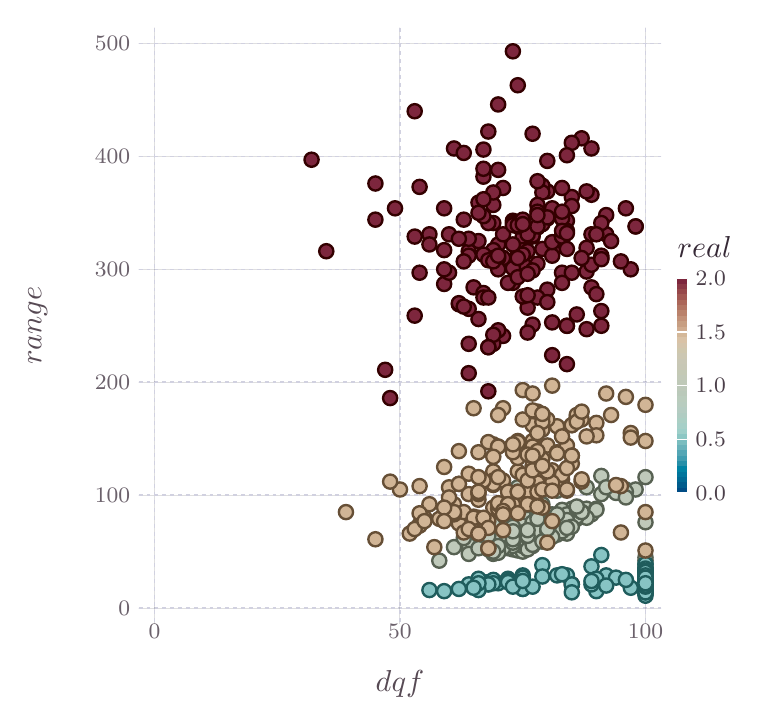
\begin{tikzpicture}[x=1mm,y=-1mm]
\definecolor{mycolorA5CFC7}{rgb}{0.65,0.81,0.78}
\definecolor{mycolor0083A3}{rgb}{0,0.51,0.64}
\definecolor{mycolorB7CBBF}{rgb}{0.72,0.8,0.75}
\definecolor{mycolor88C4C4}{rgb}{0.53,0.77,0.77}
\definecolor{mycolor7BBCC0}{rgb}{0.48,0.74,0.75}
\definecolor{mycolorAA665A}{rgb}{0.67,0.4,0.35}
\definecolor{mycolor664F35}{rgb}{0.4,0.31,0.21}
\definecolor{mycolorD2B497}{rgb}{0.82,0.71,0.59}
\definecolor{mycolorB27563}{rgb}{0.7,0.46,0.39}
\definecolor{mycolor1E5C5C}{rgb}{0.12,0.36,0.36}
\definecolor{mycolorC4C9B6}{rgb}{0.77,0.79,0.71}
\definecolor{mycolorC6C8B5}{rgb}{0.78,0.78,0.71}
\definecolor{mycolorBBCBBB}{rgb}{0.73,0.79,0.73}
\definecolor{mycolor96484A}{rgb}{0.59,0.28,0.29}
\definecolor{mycolor564A55}{rgb}{0.34,0.29,0.33}
\definecolor{mycolor004D84}{rgb}{0,0.3,0.52}
\definecolor{mycolor7E273E}{rgb}{0.49,0.15,0.24}
\definecolor{mycolor4C404B}{rgb}{0.3,0.25,0.29}
\definecolor{mycolorB1CCC2}{rgb}{0.69,0.8,0.76}
\definecolor{mycolor005B8D}{rgb}{0,0.36,0.55}
\definecolor{mycolorA05752}{rgb}{0.63,0.34,0.32}
\definecolor{mycolorC19177}{rgb}{0.76,0.57,0.47}
\definecolor{mycolorB5CCC1}{rgb}{0.71,0.8,0.76}
\definecolor{mycolorC89E82}{rgb}{0.78,0.62,0.51}
\definecolor{mycolorBA836C}{rgb}{0.73,0.51,0.42}
\definecolor{mycolorBFCAB8}{rgb}{0.75,0.79,0.72}
\definecolor{mycolorC9C7B4}{rgb}{0.79,0.78,0.71}
\definecolor{mycolorBECAB9}{rgb}{0.75,0.79,0.73}
\definecolor{mycolor8DC6C5}{rgb}{0.55,0.78,0.77}
\definecolor{mycolor000000}{rgb}{0,0,0}
\definecolor{mycolorCDAB8E}{rgb}{0.81,0.67,0.56}
\definecolor{mycolorD3B79A}{rgb}{0.83,0.72,0.6}
\definecolor{mycolor69B2BA}{rgb}{0.41,0.7,0.73}
\definecolor{mycolorD4C5AA}{rgb}{0.83,0.77,0.67}
\definecolor{mycolorABCEC4}{rgb}{0.67,0.81,0.77}
\definecolor{mycolor340000}{rgb}{0.2,0,0}
\definecolor{mycolorFFFFFF}{rgb}{1,1,1}
\definecolor{mycolor006995}{rgb}{0,0.41,0.58}
\definecolor{mycolorB9CBBD}{rgb}{0.73,0.8,0.74}
\definecolor{mycolor278FA9}{rgb}{0.15,0.56,0.66}
\definecolor{mycolor6C606B}{rgb}{0.42,0.38,0.42}
\definecolor{mycolor000000}{rgb}{0,0,0}
\definecolor{mycolor8B3844}{rgb}{0.54,0.22,0.27}
\definecolor{mycolor7E273E}{rgb}{0.49,0.15,0.24}
\definecolor{mycolorD8C3A6}{rgb}{0.85,0.76,0.65}
\definecolor{mycolor362A35}{rgb}{0.21,0.16,0.21}
\definecolor{mycolor409BAF}{rgb}{0.25,0.61,0.69}
\definecolor{mycolorCCC7B2}{rgb}{0.8,0.78,0.7}
\definecolor{mycolor55A7B5}{rgb}{0.33,0.65,0.71}
\definecolor{mycolorD0D0E0}{rgb}{0.82,0.82,0.88}
\definecolor{mycolor9ED0CB}{rgb}{0.62,0.81,0.79}
\definecolor{mycolor00769D}{rgb}{0,0.46,0.61}
\definecolor{mycolorC2C9B7}{rgb}{0.76,0.79,0.72}
\definecolor{mycolor576153}{rgb}{0.34,0.38,0.32}
\definecolor{mycolorBDCABA}{rgb}{0.74,0.79,0.73}
\definecolor{mycolorCFC6AE}{rgb}{0.81,0.78,0.68}
\begin{scope}
\begin{scope}
\draw (52.82,88.39) node [text=mycolor564A55,draw=mycolor000000,draw opacity=0,rotate around={-0: (0,1.81)},inner sep=0.0]{\fontsize{3.88mm}{4.66mm}\selectfont $\text{dqf}$};
\end{scope}
\begin{scope}
\draw (21.63,81.72) node [text=mycolor6C606B,rotate around={-0: (31.18,1.34)},inner sep=0.0]{\fontsize{2.82mm}{3.39mm}\selectfont $\text{0}$};
\draw (52.82,81.72) node [text=mycolor6C606B,rotate around={-0: (0,1.34)},inner sep=0.0]{\fontsize{2.82mm}{3.39mm}\selectfont $\text{50}$};
\draw (84,81.72) node [text=mycolor6C606B,rotate around={-0: (-31.18,1.34)},inner sep=0.0]{\fontsize{2.82mm}{3.39mm}\selectfont $\text{100}$};
\end{scope}
\begin{scope}
\begin{scope}
\draw (90.31,43.64) node [text=mycolor4C404B,rotate around={-0: (4.5,6.83)},right,inner sep=0.0]{\fontsize{2.82mm}{3.39mm}\selectfont $\text{1.5}$};
\draw (90.31,50.47) node [text=mycolor4C404B,rotate around={-0: (4.5,0)},right,inner sep=0.0]{\fontsize{2.82mm}{3.39mm}\selectfont $\text{1.0}$};
\draw (90.31,36.81) node [text=mycolor4C404B,rotate around={-0: (4.5,13.66)},right,inner sep=0.0]{\fontsize{2.82mm}{3.39mm}\selectfont $\text{2.0}$};
\draw (90.31,64.13) node [text=mycolor4C404B,rotate around={-0: (4.5,-13.66)},right,inner sep=0.0]{\fontsize{2.82mm}{3.39mm}\selectfont $\text{0.0}$};
\draw (90.31,57.3) node [text=mycolor4C404B,rotate around={-0: (4.5,-6.83)},right,inner sep=0.0]{\fontsize{2.82mm}{3.39mm}\selectfont $\text{0.5}$};
\end{scope}
\begin{scope}
\path [fill=mycolor004D84,draw=mycolor000000,draw opacity=0] (88,63.44) rectangle +(1.31,0.68);
\path [fill=mycolor005B8D,draw=mycolor000000,draw opacity=0] (88,62.76) rectangle +(1.31,0.68);
\path [fill=mycolor006995,draw=mycolor000000,draw opacity=0] (88,62.08) rectangle +(1.31,0.68);
\path [fill=mycolor00769D,draw=mycolor000000,draw opacity=0] (88,61.39) rectangle +(1.31,0.68);
\path [fill=mycolor0083A3,draw=mycolor000000,draw opacity=0] (88,60.71) rectangle +(1.31,0.68);
\path [fill=mycolor278FA9,draw=mycolor000000,draw opacity=0] (88,60.03) rectangle +(1.31,0.68);
\path [fill=mycolor409BAF,draw=mycolor000000,draw opacity=0] (88,59.35) rectangle +(1.31,0.68);
\path [fill=mycolor55A7B5,draw=mycolor000000,draw opacity=0] (88,58.66) rectangle +(1.31,0.68);
\path [fill=mycolor69B2BA,draw=mycolor000000,draw opacity=0] (88,57.98) rectangle +(1.31,0.68);
\path [fill=mycolor7BBCC0,draw=mycolor000000,draw opacity=0] (88,57.3) rectangle +(1.31,0.68);
\path [fill=mycolor8DC6C5,draw=mycolor000000,draw opacity=0] (88,56.61) rectangle +(1.31,0.68);
\path [fill=mycolor9ED0CB,draw=mycolor000000,draw opacity=0] (88,55.93) rectangle +(1.31,0.68);
\path [fill=mycolorA5CFC7,draw=mycolor000000,draw opacity=0] (88,55.25) rectangle +(1.31,0.68);
\path [fill=mycolorABCEC4,draw=mycolor000000,draw opacity=0] (88,54.57) rectangle +(1.31,0.68);
\path [fill=mycolorB1CCC2,draw=mycolor000000,draw opacity=0] (88,53.88) rectangle +(1.31,0.68);
\path [fill=mycolorB5CCC1,draw=mycolor000000,draw opacity=0] (88,53.2) rectangle +(1.31,0.68);
\path [fill=mycolorB7CBBF,draw=mycolor000000,draw opacity=0] (88,52.52) rectangle +(1.31,0.68);
\path [fill=mycolorB9CBBD,draw=mycolor000000,draw opacity=0] (88,51.83) rectangle +(1.31,0.68);
\path [fill=mycolorBBCBBB,draw=mycolor000000,draw opacity=0] (88,51.15) rectangle +(1.31,0.68);
\path [fill=mycolorBDCABA,draw=mycolor000000,draw opacity=0] (88,50.47) rectangle +(1.31,0.68);
\path [fill=mycolorBFCAB8,draw=mycolor000000,draw opacity=0] (88,49.79) rectangle +(1.31,0.68);
\path [fill=mycolorC2C9B7,draw=mycolor000000,draw opacity=0] (88,49.1) rectangle +(1.31,0.68);
\path [fill=mycolorC4C9B6,draw=mycolor000000,draw opacity=0] (88,48.42) rectangle +(1.31,0.68);
\path [fill=mycolorC6C8B5,draw=mycolor000000,draw opacity=0] (88,47.74) rectangle +(1.31,0.68);
\path [fill=mycolorC9C7B4,draw=mycolor000000,draw opacity=0] (88,47.06) rectangle +(1.31,0.68);
\path [fill=mycolorCCC7B2,draw=mycolor000000,draw opacity=0] (88,46.37) rectangle +(1.31,0.68);
\path [fill=mycolorCFC6AE,draw=mycolor000000,draw opacity=0] (88,45.69) rectangle +(1.31,0.68);
\path [fill=mycolorD4C5AA,draw=mycolor000000,draw opacity=0] (88,45.01) rectangle +(1.31,0.68);
\path [fill=mycolorD8C3A6,draw=mycolor000000,draw opacity=0] (88,44.32) rectangle +(1.31,0.68);
\path [fill=mycolorD3B79A,draw=mycolor000000,draw opacity=0] (88,43.64) rectangle +(1.31,0.68);
\path [fill=mycolorCDAB8E,draw=mycolor000000,draw opacity=0] (88,42.96) rectangle +(1.31,0.68);
\path [fill=mycolorC89E82,draw=mycolor000000,draw opacity=0] (88,42.28) rectangle +(1.31,0.68);
\path [fill=mycolorC19177,draw=mycolor000000,draw opacity=0] (88,41.59) rectangle +(1.31,0.68);
\path [fill=mycolorBA836C,draw=mycolor000000,draw opacity=0] (88,40.91) rectangle +(1.31,0.68);
\path [fill=mycolorB27563,draw=mycolor000000,draw opacity=0] (88,40.23) rectangle +(1.31,0.68);
\path [fill=mycolorAA665A,draw=mycolor000000,draw opacity=0] (88,39.54) rectangle +(1.31,0.68);
\path [fill=mycolorA05752,draw=mycolor000000,draw opacity=0] (88,38.86) rectangle +(1.31,0.68);
\path [fill=mycolor96484A,draw=mycolor000000,draw opacity=0] (88,38.18) rectangle +(1.31,0.68);
\path [fill=mycolor8B3844,draw=mycolor000000,draw opacity=0] (88,37.5) rectangle +(1.31,0.68);
\path [fill=mycolor7E273E,draw=mycolor000000,draw opacity=0] (88,36.81) rectangle +(1.31,0.68);
\begin{scope}
[line width=0.2mm]
\path [fill=mycolor004D84,draw=mycolorFFFFFF]  (88,43.64) -- (89.31,43.64);
\path [fill=mycolor005B8D,draw=mycolorFFFFFF]  (88,50.47) -- (89.31,50.47);
\path [fill=mycolor006995,draw=mycolorFFFFFF]  (88,36.81) -- (89.31,36.81);
\path [fill=mycolor00769D,draw=mycolorFFFFFF]  (88,64.13) -- (89.31,64.13);
\path [fill=mycolor0083A3,draw=mycolorFFFFFF]  (88,57.3) -- (89.31,57.3);
\end{scope}
\end{scope}
\begin{scope}
\draw (88,32.81) node [text=mycolor362A35,draw=mycolor000000,draw opacity=0,rotate around={-0: (4.5,0.19)},right,inner sep=0.0]{\fontsize{3.88mm}{4.66mm}\selectfont $\text{real}$};
\end{scope}
\end{scope}
\begin{scope}
\clip  (19.63,5) -- (86,5) -- (86,80.72) -- (19.63,80.72);
\begin{scope}
\clip  (19.63,5) -- (86,5) -- (86,80.72) -- (19.63,80.72);
\path [fill=mycolor000000,fill opacity=0,draw=mycolor000000,draw opacity=0] (19.63,5) rectangle +(66.37,75.72);
\end{scope}
\begin{scope}
[dash pattern=on 0.5mm off 0.5mm,line width=0.2mm]
\path [fill=mycolor000000,draw=mycolorD0D0E0]  (19.63,78.72) -- (86,78.72);
\path [fill=mycolor000000,draw=mycolorD0D0E0]  (19.63,64.37) -- (86,64.37);
\path [fill=mycolor000000,draw=mycolorD0D0E0]  (19.63,50.03) -- (86,50.03);
\path [fill=mycolor000000,draw=mycolorD0D0E0]  (19.63,35.69) -- (86,35.69);
\path [fill=mycolor000000,draw=mycolorD0D0E0]  (19.63,21.34) -- (86,21.34);
\path [fill=mycolor000000,draw=mycolorD0D0E0]  (19.63,7) -- (86,7);
\end{scope}
\begin{scope}
[dash pattern=on 0.5mm off 0.5mm,line width=0.2mm]
\path [fill=mycolor000000,draw=mycolorD0D0E0]  (21.63,5) -- (21.63,80.72);
\path [fill=mycolor000000,draw=mycolorD0D0E0]  (52.82,5) -- (52.82,80.72);
\path [fill=mycolor000000,draw=mycolorD0D0E0]  (84,5) -- (84,80.72);
\end{scope}
\begin{scope}
\begin{scope}
\begin{scope}
[line width=0.3mm]
\path [fill=mycolorBECAB9,draw=mycolor576153] (69.66,68.67) circle [radius=0.9];
\path [fill=mycolorBECAB9,draw=mycolor576153] (76.52,66.09) circle [radius=0.9];
\path [fill=mycolorBECAB9,draw=mycolor576153] (72.15,67.96) circle [radius=0.9];
\path [fill=mycolorBECAB9,draw=mycolor576153] (74.64,68.24) circle [radius=0.9];
\path [fill=mycolorBECAB9,draw=mycolor576153] (69.03,69.97) circle [radius=0.9];
\path [fill=mycolorBECAB9,draw=mycolor576153] (80.26,64.09) circle [radius=0.9];
\path [fill=mycolorBECAB9,draw=mycolor576153] (70.9,69.39) circle [radius=0.9];
\path [fill=mycolorBECAB9,draw=mycolor576153] (66.54,68.96) circle [radius=0.9];
\path [fill=mycolorBECAB9,draw=mycolor576153] (65.91,68.24) circle [radius=0.9];
\path [fill=mycolorBECAB9,draw=mycolor576153] (61.55,70.97) circle [radius=0.9];
\path [fill=mycolorBECAB9,draw=mycolor576153] (67.16,70.54) circle [radius=0.9];
\path [fill=mycolorBECAB9,draw=mycolor576153] (72.15,67.1) circle [radius=0.9];
\path [fill=mycolorBECAB9,draw=mycolor576153] (73.4,68.1) circle [radius=0.9];
\path [fill=mycolorBECAB9,draw=mycolor576153] (71.53,68.82) circle [radius=0.9];
\path [fill=mycolorBECAB9,draw=mycolor576153] (62.17,70.97) circle [radius=0.9];
\path [fill=mycolorBECAB9,draw=mycolor576153] (74.64,67.1) circle [radius=0.9];
\path [fill=mycolorBECAB9,draw=mycolor576153] (71.53,68.24) circle [radius=0.9];
\path [fill=mycolorBECAB9,draw=mycolor576153] (69.03,71.11) circle [radius=0.9];
\path [fill=mycolorBECAB9,draw=mycolor576153] (67.16,71.26) circle [radius=0.9];
\path [fill=mycolorBECAB9,draw=mycolor576153] (65.91,68.67) circle [radius=0.9];
\path [fill=mycolorBECAB9,draw=mycolor576153] (66.54,70.25) circle [radius=0.9];
\path [fill=mycolorBECAB9,draw=mycolor576153] (74.64,66.67) circle [radius=0.9];
\path [fill=mycolorBECAB9,draw=mycolor576153] (77.14,66.81) circle [radius=0.9];
\path [fill=mycolorBECAB9,draw=mycolor576153] (72.15,68.96) circle [radius=0.9];
\path [fill=mycolorBECAB9,draw=mycolor576153] (69.66,70.83) circle [radius=0.9];
\path [fill=mycolorBECAB9,draw=mycolor576153] (72.77,67.96) circle [radius=0.9];
\path [fill=mycolorBECAB9,draw=mycolor576153] (70.28,68.96) circle [radius=0.9];
\path [fill=mycolorBECAB9,draw=mycolor576153] (62.79,70.54) circle [radius=0.9];
\path [fill=mycolorBECAB9,draw=mycolor576153] (74.02,67.1) circle [radius=0.9];
\path [fill=mycolorBECAB9,draw=mycolor576153] (65.91,68.67) circle [radius=0.9];
\path [fill=mycolorBECAB9,draw=mycolor576153] (66.54,69.82) circle [radius=0.9];
\path [fill=mycolorBECAB9,draw=mycolor576153] (64.67,71.83) circle [radius=0.9];
\path [fill=mycolorBECAB9,draw=mycolor576153] (84,72.69) circle [radius=0.9];
\path [fill=mycolorBECAB9,draw=mycolor576153] (74.02,67.67) circle [radius=0.9];
\path [fill=mycolorBECAB9,draw=mycolor576153] (74.02,67.53) circle [radius=0.9];
\path [fill=mycolorBECAB9,draw=mycolor576153] (67.78,71.4) circle [radius=0.9];
\path [fill=mycolorBECAB9,draw=mycolor576153] (73.4,66.52) circle [radius=0.9];
\path [fill=mycolorBECAB9,draw=mycolor576153] (65.91,69.39) circle [radius=0.9];
\path [fill=mycolorBECAB9,draw=mycolor576153] (70.28,69.82) circle [radius=0.9];
\path [fill=mycolorBECAB9,draw=mycolor576153] (68.41,71.54) circle [radius=0.9];
\path [fill=mycolorBECAB9,draw=mycolor576153] (65.29,70.97) circle [radius=0.9];
\path [fill=mycolorBECAB9,draw=mycolor576153] (73.4,67.96) circle [radius=0.9];
\path [fill=mycolorBECAB9,draw=mycolor576153] (59.68,70.97) circle [radius=0.9];
\path [fill=mycolorBECAB9,draw=mycolor576153] (72.15,68.1) circle [radius=0.9];
\path [fill=mycolorBECAB9,draw=mycolor576153] (69.03,68.96) circle [radius=0.9];
\path [fill=mycolorBECAB9,draw=mycolor576153] (64.04,70.54) circle [radius=0.9];
\path [fill=mycolorBECAB9,draw=mycolor576153] (84,67.81) circle [radius=0.9];
\path [fill=mycolorBECAB9,draw=mycolor576153] (72.77,67.38) circle [radius=0.9];
\path [fill=mycolorBECAB9,draw=mycolor576153] (67.78,68.39) circle [radius=0.9];
\path [fill=mycolorBECAB9,draw=mycolor576153] (66.54,69.25) circle [radius=0.9];
\path [fill=mycolorBECAB9,draw=mycolor576153] (69.66,67.67) circle [radius=0.9];
\path [fill=mycolorBECAB9,draw=mycolor576153] (78.39,64.23) circle [radius=0.9];
\path [fill=mycolorBECAB9,draw=mycolor576153] (70.9,65.95) circle [radius=0.9];
\path [fill=mycolorBECAB9,draw=mycolor576153] (65.29,70.97) circle [radius=0.9];
\path [fill=mycolorBECAB9,draw=mycolor576153] (65.29,70.54) circle [radius=0.9];
\path [fill=mycolorBECAB9,draw=mycolor576153] (68.41,69.11) circle [radius=0.9];
\path [fill=mycolorBECAB9,draw=mycolor576153] (70.9,69.82) circle [radius=0.9];
\path [fill=mycolorBECAB9,draw=mycolor576153] (76.52,63.37) circle [radius=0.9];
\path [fill=mycolorBECAB9,draw=mycolor576153] (71.53,68.39) circle [radius=0.9];
\path [fill=mycolorBECAB9,draw=mycolor576153] (69.66,70.4) circle [radius=0.9];
\path [fill=mycolorBECAB9,draw=mycolor576153] (81.51,63.65) circle [radius=0.9];
\path [fill=mycolorBECAB9,draw=mycolor576153] (72.77,63.51) circle [radius=0.9];
\path [fill=mycolorBECAB9,draw=mycolor576153] (69.66,70.4) circle [radius=0.9];
\path [fill=mycolorBECAB9,draw=mycolor576153] (74.64,66.38) circle [radius=0.9];
\path [fill=mycolorBECAB9,draw=mycolor576153] (67.78,66.52) circle [radius=0.9];
\path [fill=mycolorBECAB9,draw=mycolor576153] (70.28,68.67) circle [radius=0.9];
\path [fill=mycolorBECAB9,draw=mycolor576153] (75.27,67.38) circle [radius=0.9];
\path [fill=mycolorBECAB9,draw=mycolor576153] (72.15,67.38) circle [radius=0.9];
\path [fill=mycolorBECAB9,draw=mycolor576153] (66.54,71.11) circle [radius=0.9];
\path [fill=mycolorBECAB9,draw=mycolor576153] (65.29,69.25) circle [radius=0.9];
\path [fill=mycolorBECAB9,draw=mycolor576153] (71.53,68.82) circle [radius=0.9];
\path [fill=mycolorBECAB9,draw=mycolor576153] (73.4,68.39) circle [radius=0.9];
\path [fill=mycolorBECAB9,draw=mycolor576153] (69.66,68.1) circle [radius=0.9];
\path [fill=mycolorBECAB9,draw=mycolor576153] (72.15,68.82) circle [radius=0.9];
\path [fill=mycolorBECAB9,draw=mycolor576153] (65.29,67.53) circle [radius=0.9];
\path [fill=mycolorBECAB9,draw=mycolor576153] (70.28,68.1) circle [radius=0.9];
\path [fill=mycolorBECAB9,draw=mycolor576153] (72.15,67.81) circle [radius=0.9];
\path [fill=mycolorBECAB9,draw=mycolor576153] (65.91,67.96) circle [radius=0.9];
\path [fill=mycolorBECAB9,draw=mycolor576153] (77.76,66.09) circle [radius=0.9];
\path [fill=mycolorBECAB9,draw=mycolor576153] (74.02,68.53) circle [radius=0.9];
\path [fill=mycolorBECAB9,draw=mycolor576153] (82.75,63.65) circle [radius=0.9];
\path [fill=mycolorBECAB9,draw=mycolor576153] (71.53,66.81) circle [radius=0.9];
\path [fill=mycolorBECAB9,draw=mycolor576153] (67.16,70.54) circle [radius=0.9];
\path [fill=mycolorBECAB9,draw=mycolor576153] (72.15,68.39) circle [radius=0.9];
\path [fill=mycolorBECAB9,draw=mycolor576153] (72.77,68.39) circle [radius=0.9];
\path [fill=mycolorBECAB9,draw=mycolor576153] (74.64,66.95) circle [radius=0.9];
\path [fill=mycolorBECAB9,draw=mycolor576153] (74.02,66.67) circle [radius=0.9];
\path [fill=mycolorBECAB9,draw=mycolor576153] (71.53,68.39) circle [radius=0.9];
\path [fill=mycolorBECAB9,draw=mycolor576153] (78.39,61.93) circle [radius=0.9];
\path [fill=mycolorBECAB9,draw=mycolor576153] (77.76,66.24) circle [radius=0.9];
\path [fill=mycolorBECAB9,draw=mycolor576153] (68.41,70.83) circle [radius=0.9];
\path [fill=mycolorBECAB9,draw=mycolor576153] (81.51,63.94) circle [radius=0.9];
\path [fill=mycolorBECAB9,draw=mycolor576153] (70.9,70.25) circle [radius=0.9];
\path [fill=mycolorBECAB9,draw=mycolor576153] (67.78,68.67) circle [radius=0.9];
\path [fill=mycolorBECAB9,draw=mycolor576153] (68.41,68.67) circle [radius=0.9];
\path [fill=mycolorBECAB9,draw=mycolor576153] (66.54,70.11) circle [radius=0.9];
\path [fill=mycolorBECAB9,draw=mycolor576153] (81.51,64.66) circle [radius=0.9];
\path [fill=mycolorBECAB9,draw=mycolor576153] (69.66,67.53) circle [radius=0.9];
\path [fill=mycolorBECAB9,draw=mycolor576153] (65.91,68.82) circle [radius=0.9];
\path [fill=mycolorBECAB9,draw=mycolor576153] (72.77,68.1) circle [radius=0.9];
\path [fill=mycolorBECAB9,draw=mycolor576153] (74.64,66.09) circle [radius=0.9];
\path [fill=mycolorBECAB9,draw=mycolor576153] (79.01,63.37) circle [radius=0.9];
\path [fill=mycolorBECAB9,draw=mycolor576153] (70.9,68.39) circle [radius=0.9];
\path [fill=mycolorBECAB9,draw=mycolor576153] (64.67,68.1) circle [radius=0.9];
\path [fill=mycolorBECAB9,draw=mycolor576153] (84,62.08) circle [radius=0.9];
\path [fill=mycolorBECAB9,draw=mycolor576153] (75.89,67.1) circle [radius=0.9];
\path [fill=mycolorBECAB9,draw=mycolor576153] (74.64,67.53) circle [radius=0.9];
\path [fill=mycolorBECAB9,draw=mycolor576153] (71.53,66.81) circle [radius=0.9];
\path [fill=mycolorBECAB9,draw=mycolor576153] (74.64,67.81) circle [radius=0.9];
\path [fill=mycolorBECAB9,draw=mycolor576153] (62.79,69.97) circle [radius=0.9];
\path [fill=mycolorBECAB9,draw=mycolor576153] (62.17,71.11) circle [radius=0.9];
\path [fill=mycolorBECAB9,draw=mycolor576153] (61.55,70.68) circle [radius=0.9];
\path [fill=mycolorBECAB9,draw=mycolor576153] (70.28,68.82) circle [radius=0.9];
\path [fill=mycolorBECAB9,draw=mycolor576153] (69.03,71.26) circle [radius=0.9];
\path [fill=mycolorBECAB9,draw=mycolor576153] (70.28,70.25) circle [radius=0.9];
\path [fill=mycolorBECAB9,draw=mycolor576153] (64.67,70.11) circle [radius=0.9];
\path [fill=mycolorBECAB9,draw=mycolor576153] (70.28,69.97) circle [radius=0.9];
\path [fill=mycolorBECAB9,draw=mycolor576153] (70.28,69.97) circle [radius=0.9];
\path [fill=mycolorBECAB9,draw=mycolor576153] (74.02,69.25) circle [radius=0.9];
\path [fill=mycolorBECAB9,draw=mycolor576153] (67.78,67.67) circle [radius=0.9];
\path [fill=mycolorBECAB9,draw=mycolor576153] (60.92,69.82) circle [radius=0.9];
\path [fill=mycolorBECAB9,draw=mycolor576153] (73.4,68.67) circle [radius=0.9];
\path [fill=mycolorBECAB9,draw=mycolor576153] (72.77,69.39) circle [radius=0.9];
\path [fill=mycolorBECAB9,draw=mycolor576153] (67.78,63.37) circle [radius=0.9];
\path [fill=mycolorBECAB9,draw=mycolor576153] (69.66,69.25) circle [radius=0.9];
\path [fill=mycolorBECAB9,draw=mycolor576153] (68.41,69.11) circle [radius=0.9];
\path [fill=mycolorBECAB9,draw=mycolor576153] (74.02,67.38) circle [radius=0.9];
\path [fill=mycolorBECAB9,draw=mycolor576153] (69.03,69.25) circle [radius=0.9];
\path [fill=mycolorBECAB9,draw=mycolor576153] (69.66,66.67) circle [radius=0.9];
\path [fill=mycolorBECAB9,draw=mycolor576153] (72.15,67.67) circle [radius=0.9];
\path [fill=mycolorBECAB9,draw=mycolor576153] (68.41,69.39) circle [radius=0.9];
\path [fill=mycolorBECAB9,draw=mycolor576153] (67.78,68.67) circle [radius=0.9];
\path [fill=mycolorBECAB9,draw=mycolor576153] (73.4,67.1) circle [radius=0.9];
\path [fill=mycolorBECAB9,draw=mycolor576153] (72.77,63.8) circle [radius=0.9];
\path [fill=mycolorBECAB9,draw=mycolor576153] (69.66,69.11) circle [radius=0.9];
\path [fill=mycolorBECAB9,draw=mycolor576153] (76.52,67.24) circle [radius=0.9];
\path [fill=mycolorBECAB9,draw=mycolor576153] (75.27,67.1) circle [radius=0.9];
\path [fill=mycolorBECAB9,draw=mycolor576153] (72.15,66.81) circle [radius=0.9];
\path [fill=mycolorBECAB9,draw=mycolor576153] (72.15,68.39) circle [radius=0.9];
\path [fill=mycolorBECAB9,draw=mycolor576153] (64.67,71.54) circle [radius=0.9];
\path [fill=mycolorBECAB9,draw=mycolor576153] (67.16,69.11) circle [radius=0.9];
\path [fill=mycolorBECAB9,draw=mycolor576153] (69.03,68.82) circle [radius=0.9];
\path [fill=mycolorBECAB9,draw=mycolor576153] (69.03,67.38) circle [radius=0.9];
\path [fill=mycolorBECAB9,draw=mycolor576153] (67.16,70.83) circle [radius=0.9];
\path [fill=mycolorBECAB9,draw=mycolor576153] (65.91,71.11) circle [radius=0.9];
\path [fill=mycolorBECAB9,draw=mycolor576153] (64.04,71.26) circle [radius=0.9];
\path [fill=mycolorBECAB9,draw=mycolor576153] (72.77,67.1) circle [radius=0.9];
\path [fill=mycolorBECAB9,draw=mycolor576153] (74.02,68.39) circle [radius=0.9];
\path [fill=mycolorBECAB9,draw=mycolor576153] (69.03,68.82) circle [radius=0.9];
\path [fill=mycolorBECAB9,draw=mycolor576153] (74.02,66.81) circle [radius=0.9];
\path [fill=mycolorBECAB9,draw=mycolor576153] (69.03,69.11) circle [radius=0.9];
\path [fill=mycolorBECAB9,draw=mycolor576153] (70.28,67.96) circle [radius=0.9];
\path [fill=mycolorBECAB9,draw=mycolor576153] (70.28,66.81) circle [radius=0.9];
\path [fill=mycolorBECAB9,draw=mycolor576153] (70.9,65.52) circle [radius=0.9];
\path [fill=mycolorBECAB9,draw=mycolor576153] (67.16,70.4) circle [radius=0.9];
\path [fill=mycolorBECAB9,draw=mycolor576153] (70.28,68.39) circle [radius=0.9];
\path [fill=mycolorBECAB9,draw=mycolor576153] (73.4,68.53) circle [radius=0.9];
\path [fill=mycolorBECAB9,draw=mycolor576153] (75.89,66.52) circle [radius=0.9];
\path [fill=mycolorBECAB9,draw=mycolor576153] (61.55,71.83) circle [radius=0.9];
\path [fill=mycolorBECAB9,draw=mycolor576153] (69.66,70.68) circle [radius=0.9];
\path [fill=mycolorBECAB9,draw=mycolor576153] (64.67,69.54) circle [radius=0.9];
\path [fill=mycolorBECAB9,draw=mycolor576153] (70.28,68.1) circle [radius=0.9];
\path [fill=mycolorBECAB9,draw=mycolor576153] (65.29,71.69) circle [radius=0.9];
\path [fill=mycolorBECAB9,draw=mycolor576153] (68.41,68.24) circle [radius=0.9];
\path [fill=mycolorBECAB9,draw=mycolor576153] (69.66,67.81) circle [radius=0.9];
\path [fill=mycolorBECAB9,draw=mycolor576153] (62.79,71.11) circle [radius=0.9];
\path [fill=mycolorBECAB9,draw=mycolor576153] (72.77,68.82) circle [radius=0.9];
\path [fill=mycolorBECAB9,draw=mycolor576153] (73.4,66.24) circle [radius=0.9];
\path [fill=mycolorBECAB9,draw=mycolor576153] (73.4,68.96) circle [radius=0.9];
\path [fill=mycolorBECAB9,draw=mycolor576153] (84,72.26) circle [radius=0.9];
\path [fill=mycolorBECAB9,draw=mycolor576153] (74.02,66.81) circle [radius=0.9];
\path [fill=mycolorBECAB9,draw=mycolor576153] (75.27,66.09) circle [radius=0.9];
\path [fill=mycolorBECAB9,draw=mycolor576153] (65.29,70.83) circle [radius=0.9];
\path [fill=mycolorBECAB9,draw=mycolor576153] (57.81,72.69) circle [radius=0.9];
\path [fill=mycolorBECAB9,draw=mycolor576153] (70.9,69.11) circle [radius=0.9];
\path [fill=mycolorBECAB9,draw=mycolor576153] (70.9,69.25) circle [radius=0.9];
\path [fill=mycolorBECAB9,draw=mycolor576153] (71.53,67.67) circle [radius=0.9];
\path [fill=mycolorBECAB9,draw=mycolor576153] (75.89,66.52) circle [radius=0.9];
\path [fill=mycolorBECAB9,draw=mycolor576153] (70.28,69.11) circle [radius=0.9];
\path [fill=mycolorBECAB9,draw=mycolor576153] (74.02,67.53) circle [radius=0.9];
\path [fill=mycolorBECAB9,draw=mycolor576153] (71.53,68.96) circle [radius=0.9];
\path [fill=mycolorBECAB9,draw=mycolor576153] (68.41,69.11) circle [radius=0.9];
\path [fill=mycolorBECAB9,draw=mycolor576153] (70.28,66.81) circle [radius=0.9];
\path [fill=mycolorBECAB9,draw=mycolor576153] (72.15,67.38) circle [radius=0.9];
\path [fill=mycolorBECAB9,draw=mycolor576153] (64.67,71.54) circle [radius=0.9];
\path [fill=mycolorBECAB9,draw=mycolor576153] (70.9,70.25) circle [radius=0.9];
\path [fill=mycolorBECAB9,draw=mycolor576153] (75.27,65.81) circle [radius=0.9];
\path [fill=mycolorBECAB9,draw=mycolor576153] (69.03,69.54) circle [radius=0.9];
\path [fill=mycolorBECAB9,draw=mycolor576153] (72.15,69.68) circle [radius=0.9];
\path [fill=mycolorBECAB9,draw=mycolor576153] (67.16,69.97) circle [radius=0.9];
\path [fill=mycolorBECAB9,draw=mycolor576153] (67.16,68.39) circle [radius=0.9];
\path [fill=mycolorBECAB9,draw=mycolor576153] (84,73.55) circle [radius=0.9];
\path [fill=mycolorBECAB9,draw=mycolor576153] (74.64,68.39) circle [radius=0.9];
\path [fill=mycolorBECAB9,draw=mycolor576153] (69.03,68.82) circle [radius=0.9];
\path [fill=mycolorBECAB9,draw=mycolor576153] (74.02,68.53) circle [radius=0.9];
\path [fill=mycolorBECAB9,draw=mycolor576153] (64.04,69.54) circle [radius=0.9];
\path [fill=mycolorBECAB9,draw=mycolor576153] (70.28,67.38) circle [radius=0.9];
\path [fill=mycolorBECAB9,draw=mycolor576153] (67.16,68.96) circle [radius=0.9];
\path [fill=mycolorBECAB9,draw=mycolor576153] (72.77,66.81) circle [radius=0.9];
\path [fill=mycolorBECAB9,draw=mycolor576153] (71.53,68.67) circle [radius=0.9];
\path [fill=mycolor7E273E,draw=mycolor340000] (74.64,75.7) circle [radius=0.9];
\path [fill=mycolor7E273E,draw=mycolor340000] (76.52,35.97) circle [radius=0.9];
\path [fill=mycolor7E273E,draw=mycolor340000] (50.94,48.45) circle [radius=0.9];
\path [fill=mycolor7E273E,draw=mycolor340000] (79.01,31.24) circle [radius=0.9];
\path [fill=mycolor7E273E,draw=mycolor340000] (77.14,20.34) circle [radius=0.9];
\path [fill=mycolor7E273E,draw=mycolor340000] (70.28,30.38) circle [radius=0.9];
\path [fill=mycolor7E273E,draw=mycolor340000] (59.68,20.34) circle [radius=0.9];
\path [fill=mycolor7E273E,draw=mycolor340000] (64.04,51.18) circle [radius=0.9];
\path [fill=mycolor7E273E,draw=mycolor340000] (65.91,44.15) circle [radius=0.9];
\path [fill=mycolor7E273E,draw=mycolor340000] (75.27,41.42) circle [radius=0.9];
\path [fill=mycolor7E273E,draw=mycolor340000] (72.15,46.59) circle [radius=0.9];
\path [fill=mycolor7E273E,draw=mycolor340000] (82.13,35.69) circle [radius=0.9];
\path [fill=mycolor7E273E,draw=mycolor340000] (58.43,37.55) circle [radius=0.9];
\path [fill=mycolor7E273E,draw=mycolor340000] (75.89,19.05) circle [radius=0.9];
\path [fill=mycolor7E273E,draw=mycolor340000] (69.03,40.56) circle [radius=0.9];
\path [fill=mycolor7E273E,draw=mycolor340000] (77.14,37.98) circle [radius=0.9];
\path [fill=mycolor7E273E,draw=mycolor340000] (43.46,33.39) circle [radius=0.9];
\path [fill=mycolor7E273E,draw=mycolor340000] (72.77,32.82) circle [radius=0.9];
\path [fill=mycolor7E273E,draw=mycolor340000] (62.79,32.1) circle [radius=0.9];
\path [fill=mycolor7E273E,draw=mycolor340000] (68.41,34.83) circle [radius=0.9];
\path [fill=mycolor7E273E,draw=mycolor340000] (67.78,12.31) circle [radius=0.9];
\path [fill=mycolor7E273E,draw=mycolor340000] (61.55,33.39) circle [radius=0.9];
\path [fill=mycolor7E273E,draw=mycolor340000] (59.05,31.24) circle [radius=0.9];
\path [fill=mycolor7E273E,draw=mycolor340000] (55.31,36.12) circle [radius=0.9];
\path [fill=mycolor7E273E,draw=mycolor340000] (62.17,37.98) circle [radius=0.9];
\path [fill=mycolor7E273E,draw=mycolor340000] (71.53,25.79) circle [radius=0.9];
\path [fill=mycolor7E273E,draw=mycolor340000] (65.91,25.36) circle [radius=0.9];
\path [fill=mycolor7E273E,draw=mycolor340000] (62.79,42) circle [radius=0.9];
\path [fill=mycolor7E273E,draw=mycolor340000] (69.66,42.71) circle [radius=0.9];
\path [fill=mycolor7E273E,draw=mycolor340000] (79.01,28.8) circle [radius=0.9];
\path [fill=mycolor7E273E,draw=mycolor340000] (64.67,27.51) circle [radius=0.9];
\path [fill=mycolor7E273E,draw=mycolor340000] (74.64,19.62) circle [radius=0.9];
\path [fill=mycolor7E273E,draw=mycolor340000] (65.29,32.53) circle [radius=0.9];
\path [fill=mycolor7E273E,draw=mycolor340000] (69.66,31.53) circle [radius=0.9];
\path [fill=mycolor7E273E,draw=mycolor340000] (68.41,31.53) circle [radius=0.9];
\path [fill=mycolor7E273E,draw=mycolor340000] (68.41,33.25) circle [radius=0.9];
\path [fill=mycolor7E273E,draw=mycolor340000] (71.53,29.23) circle [radius=0.9];
\path [fill=mycolor7E273E,draw=mycolor340000] (77.14,31.24) circle [radius=0.9];
\path [fill=mycolor7E273E,draw=mycolor340000] (69.66,31.38) circle [radius=0.9];
\path [fill=mycolor7E273E,draw=mycolor340000] (67.16,29.52) circle [radius=0.9];
\path [fill=mycolor7E273E,draw=mycolor340000] (58.43,33.25) circle [radius=0.9];
\path [fill=mycolor7E273E,draw=mycolor340000] (64.67,29.81) circle [radius=0.9];
\path [fill=mycolor7E273E,draw=mycolor340000] (61.55,45.15) circle [radius=0.9];
\path [fill=mycolor7E273E,draw=mycolor340000] (67.16,29.81) circle [radius=0.9];
\path [fill=mycolor7E273E,draw=mycolor340000] (59.05,36.12) circle [radius=0.9];
\path [fill=mycolor7E273E,draw=mycolor340000] (61.55,33.96) circle [radius=0.9];
\path [fill=mycolor7E273E,draw=mycolor340000] (67.16,35.26) circle [radius=0.9];
\path [fill=mycolor7E273E,draw=mycolor340000] (49.7,29.38) circle [radius=0.9];
\path [fill=mycolor7E273E,draw=mycolor340000] (62.79,27.22) circle [radius=0.9];
\path [fill=mycolor7E273E,draw=mycolor340000] (73.4,29.23) circle [radius=0.9];
\path [fill=mycolor7E273E,draw=mycolor340000] (67.16,35.54) circle [radius=0.9];
\path [fill=mycolor7E273E,draw=mycolor340000] (65.29,14.75) circle [radius=0.9];
\path [fill=mycolor7E273E,draw=mycolor340000] (82.75,30.24) circle [radius=0.9];
\path [fill=mycolor7E273E,draw=mycolor340000] (70.28,34.97) circle [radius=0.9];
\path [fill=mycolor7E273E,draw=mycolor340000] (64.67,33.25) circle [radius=0.9];
\path [fill=mycolor7E273E,draw=mycolor340000] (64.67,25.93) circle [radius=0.9];
\path [fill=mycolor7E273E,draw=mycolor340000] (64.04,29.81) circle [radius=0.9];
\path [fill=mycolor7E273E,draw=mycolor340000] (70.9,25.07) circle [radius=0.9];
\path [fill=mycolor7E273E,draw=mycolor340000] (77.14,26.22) circle [radius=0.9];
\path [fill=mycolor7E273E,draw=mycolor340000] (70.9,25.93) circle [radius=0.9];
\path [fill=mycolor7E273E,draw=mycolor340000] (78.39,34.25) circle [radius=0.9];
\path [fill=mycolor7E273E,draw=mycolor340000] (70.28,27.51) circle [radius=0.9];
\path [fill=mycolor7E273E,draw=mycolor340000] (67.78,33.82) circle [radius=0.9];
\path [fill=mycolor7E273E,draw=mycolor340000] (69.03,31.24) circle [radius=0.9];
\path [fill=mycolor7E273E,draw=mycolor340000] (67.78,30.24) circle [radius=0.9];
\path [fill=mycolor7E273E,draw=mycolor340000] (71.53,38.27) circle [radius=0.9];
\path [fill=mycolor7E273E,draw=mycolor340000] (74.64,26.51) circle [radius=0.9];
\path [fill=mycolor7E273E,draw=mycolor340000] (74.02,29.52) circle [radius=0.9];
\path [fill=mycolor7E273E,draw=mycolor340000] (70.9,29.95) circle [radius=0.9];
\path [fill=mycolor7E273E,draw=mycolor340000] (70.28,28.37) circle [radius=0.9];
\path [fill=mycolor7E273E,draw=mycolor340000] (73.4,36.12) circle [radius=0.9];
\path [fill=mycolor7E273E,draw=mycolor340000] (79.63,32.1) circle [radius=0.9];
\path [fill=mycolor7E273E,draw=mycolor340000] (81.51,27.94) circle [radius=0.9];
\path [fill=mycolor7E273E,draw=mycolor340000] (67.78,29.81) circle [radius=0.9];
\path [fill=mycolor7E273E,draw=mycolor340000] (70.9,33.1) circle [radius=0.9];
\path [fill=mycolor7E273E,draw=mycolor340000] (70.28,24.5) circle [radius=0.9];
\path [fill=mycolor7E273E,draw=mycolor340000] (76.52,25.79) circle [radius=0.9];
\path [fill=mycolor7E273E,draw=mycolor340000] (72.15,27.94) circle [radius=0.9];
\path [fill=mycolor7E273E,draw=mycolor340000] (71.53,29.09) circle [radius=0.9];
\path [fill=mycolor7E273E,draw=mycolor340000] (70.28,30.24) circle [radius=0.9];
\path [fill=mycolor7E273E,draw=mycolor340000] (77.14,35.11) circle [radius=0.9];
\path [fill=mycolor7E273E,draw=mycolor340000] (73.4,25.36) circle [radius=0.9];
\path [fill=mycolor7E273E,draw=mycolor340000] (74.02,21.2) circle [radius=0.9];
\path [fill=mycolor7E273E,draw=mycolor340000] (63.42,23.92) circle [radius=0.9];
\path [fill=mycolor7E273E,draw=mycolor340000] (60.92,29.38) circle [radius=0.9];
\path [fill=mycolor7E273E,draw=mycolor340000] (63.42,20.48) circle [radius=0.9];
\path [fill=mycolor7E273E,draw=mycolor340000] (65.91,31.24) circle [radius=0.9];
\path [fill=mycolor7E273E,draw=mycolor340000] (70.28,28.8) circle [radius=0.9];
\path [fill=mycolor7E273E,draw=mycolor340000] (73.4,29.23) circle [radius=0.9];
\path [fill=mycolor7E273E,draw=mycolor340000] (67.16,30.09) circle [radius=0.9];
\path [fill=mycolor7E273E,draw=mycolor340000] (68.41,29.81) circle [radius=0.9];
\path [fill=mycolor7E273E,draw=mycolor340000] (82.75,30.24) circle [radius=0.9];
\path [fill=mycolor7E273E,draw=mycolor340000] (71.53,21.92) circle [radius=0.9];
\path [fill=mycolor7E273E,draw=mycolor340000] (69.03,33.39) circle [radius=0.9];
\path [fill=mycolor7E273E,draw=mycolor340000] (74.02,30.81) circle [radius=0.9];
\path [fill=mycolor7E273E,draw=mycolor340000] (64.67,34.25) circle [radius=0.9];
\path [fill=mycolor7E273E,draw=mycolor340000] (56.56,31.24) circle [radius=0.9];
\path [fill=mycolor7E273E,draw=mycolor340000] (49.7,24.79) circle [radius=0.9];
\path [fill=mycolor7E273E,draw=mycolor340000] (41.59,21.77) circle [radius=0.9];
\path [fill=mycolor7E273E,draw=mycolor340000] (68.41,33.82) circle [radius=0.9];
\path [fill=mycolor7E273E,draw=mycolor340000] (54.69,31.53) circle [radius=0.9];
\path [fill=mycolor7E273E,draw=mycolor340000] (51.57,52.04) circle [radius=0.9];
\path [fill=mycolor7E273E,draw=mycolor340000] (67.16,37.41) circle [radius=0.9];
\path [fill=mycolor7E273E,draw=mycolor340000] (64.04,18.19) circle [radius=0.9];
\path [fill=mycolor7E273E,draw=mycolor340000] (69.03,43.72) circle [radius=0.9];
\path [fill=mycolor7E273E,draw=mycolor340000] (61.55,31.81) circle [radius=0.9];
\path [fill=mycolor7E273E,draw=mycolor340000] (74.64,27.65) circle [radius=0.9];
\path [fill=mycolor7E273E,draw=mycolor340000] (55.31,25.22) circle [radius=0.9];
\path [fill=mycolor7E273E,draw=mycolor340000] (70.28,39.27) circle [radius=0.9];
\path [fill=mycolor7E273E,draw=mycolor340000] (68.41,39.13) circle [radius=0.9];
\path [fill=mycolor7E273E,draw=mycolor340000] (65.29,23.06) circle [radius=0.9];
\path [fill=mycolor7E273E,draw=mycolor340000] (78.39,33.96) circle [radius=0.9];
\path [fill=mycolor7E273E,draw=mycolor340000] (63.42,28.94) circle [radius=0.9];
\path [fill=mycolor7E273E,draw=mycolor340000] (78.39,29.81) circle [radius=0.9];
\path [fill=mycolor7E273E,draw=mycolor340000] (67.16,8) circle [radius=0.9];
\path [fill=mycolor7E273E,draw=mycolor340000] (78.39,42.86) circle [radius=0.9];
\path [fill=mycolor7E273E,draw=mycolor340000] (76.52,43.29) circle [radius=0.9];
\path [fill=mycolor7E273E,draw=mycolor340000] (76.52,32.96) circle [radius=0.9];
\path [fill=mycolor7E273E,draw=mycolor340000] (60.3,40.13) circle [radius=0.9];
\path [fill=mycolor7E273E,draw=mycolor340000] (67.78,30.09) circle [radius=0.9];
\path [fill=mycolor7E273E,draw=mycolor340000] (66.54,37.41) circle [radius=0.9];
\path [fill=mycolor7E273E,draw=mycolor340000] (78.39,34.4) circle [radius=0.9];
\path [fill=mycolor7E273E,draw=mycolor340000] (67.16,32.53) circle [radius=0.9];
\path [fill=mycolor7E273E,draw=mycolor340000] (69.03,38.98) circle [radius=0.9];
\path [fill=mycolor7E273E,draw=mycolor340000] (69.66,18.47) circle [radius=0.9];
\path [fill=mycolor7E273E,draw=mycolor340000] (62.79,28.51) circle [radius=0.9];
\path [fill=mycolor7E273E,draw=mycolor340000] (64.67,45.15) circle [radius=0.9];
\path [fill=mycolor7E273E,draw=mycolor340000] (67.78,34.25) circle [radius=0.9];
\path [fill=mycolor7E273E,draw=mycolor340000] (63.42,33.82) circle [radius=0.9];
\path [fill=mycolor7E273E,draw=mycolor340000] (77.76,31.24) circle [radius=0.9];
\path [fill=mycolor7E273E,draw=mycolor340000] (75.89,34.25) circle [radius=0.9];
\path [fill=mycolor7E273E,draw=mycolor340000] (69.66,35.83) circle [radius=0.9];
\path [fill=mycolor7E273E,draw=mycolor340000] (74.64,36.12) circle [radius=0.9];
\path [fill=mycolor7E273E,draw=mycolor340000] (73.4,32.1) circle [radius=0.9];
\path [fill=mycolor7E273E,draw=mycolor340000] (73.4,37.41) circle [radius=0.9];
\path [fill=mycolor7E273E,draw=mycolor340000] (61.55,40.71) circle [radius=0.9];
\path [fill=mycolor7E273E,draw=mycolor340000] (60.3,39.99) circle [radius=0.9];
\path [fill=mycolor7E273E,draw=mycolor340000] (72.15,42.43) circle [radius=0.9];
\path [fill=mycolor7E273E,draw=mycolor340000] (67.78,36.69) circle [radius=0.9];
\path [fill=mycolor7E273E,draw=mycolor340000] (73.4,28.37) circle [radius=0.9];
\path [fill=mycolor7E273E,draw=mycolor340000] (64.04,34.54) circle [radius=0.9];
\path [fill=mycolor7E273E,draw=mycolor340000] (72.15,33.96) circle [radius=0.9];
\path [fill=mycolor7E273E,draw=mycolor340000] (54.69,41.57) circle [radius=0.9];
\path [fill=mycolor7E273E,draw=mycolor340000] (65.29,43.43) circle [radius=0.9];
\path [fill=mycolor7E273E,draw=mycolor340000] (65.91,34.25) circle [radius=0.9];
\path [fill=mycolor7E273E,draw=mycolor340000] (65.91,34.25) circle [radius=0.9];
\path [fill=mycolor7E273E,draw=mycolor340000] (65.29,34.25) circle [radius=0.9];
\path [fill=mycolor7E273E,draw=mycolor340000] (65.29,35.69) circle [radius=0.9];
\path [fill=mycolor7E273E,draw=mycolor340000] (63.42,38.7) circle [radius=0.9];
\path [fill=mycolor7E273E,draw=mycolor340000] (60.3,31.81) circle [radius=0.9];
\path [fill=mycolor7E273E,draw=mycolor340000] (63.42,26.79) circle [radius=0.9];
\path [fill=mycolor7E273E,draw=mycolor340000] (68.41,29.38) circle [radius=0.9];
\path [fill=mycolor7E273E,draw=mycolor340000] (64.67,34.68) circle [radius=0.9];
\path [fill=mycolor7E273E,draw=mycolor340000] (58.43,35.69) circle [radius=0.9];
\path [fill=mycolor7E273E,draw=mycolor340000] (72.15,32.24) circle [radius=0.9];
\path [fill=mycolor7E273E,draw=mycolor340000] (77.76,38.84) circle [radius=0.9];
\path [fill=mycolor7E273E,draw=mycolor340000] (63.42,39.27) circle [radius=0.9];
\path [fill=mycolor7E273E,draw=mycolor340000] (73.4,31.53) circle [radius=0.9];
\path [fill=mycolor7E273E,draw=mycolor340000] (73.4,31.53) circle [radius=0.9];
\path [fill=mycolor7E273E,draw=mycolor340000] (64.67,44) circle [radius=0.9];
\path [fill=mycolor7E273E,draw=mycolor340000] (80.88,34.68) circle [radius=0.9];
\path [fill=mycolor7E273E,draw=mycolor340000] (74.02,33.1) circle [radius=0.9];
\path [fill=mycolor7E273E,draw=mycolor340000] (60.92,20.91) circle [radius=0.9];
\path [fill=mycolor7E273E,draw=mycolor340000] (60.92,40.42) circle [radius=0.9];
\path [fill=mycolor7E273E,draw=mycolor340000] (73.4,30.81) circle [radius=0.9];
\path [fill=mycolor7E273E,draw=mycolor340000] (64.04,45.58) circle [radius=0.9];
\path [fill=mycolor7E273E,draw=mycolor340000] (64.04,45.58) circle [radius=0.9];
\path [fill=mycolor7E273E,draw=mycolor340000] (61.55,48.88) circle [radius=0.9];
\path [fill=mycolor7E273E,draw=mycolor340000] (71.53,39.85) circle [radius=0.9];
\path [fill=mycolor7E273E,draw=mycolor340000] (60.92,34.68) circle [radius=0.9];
\path [fill=mycolor7E273E,draw=mycolor340000] (74.02,42.86) circle [radius=0.9];
\path [fill=mycolor7E273E,draw=mycolor340000] (74.02,42.86) circle [radius=0.9];
\path [fill=mycolor7E273E,draw=mycolor340000] (58.43,27.94) circle [radius=0.9];
\path [fill=mycolor7E273E,draw=mycolor340000] (69.03,36.26) circle [radius=0.9];
\path [fill=mycolor7E273E,draw=mycolor340000] (63.42,22.92) circle [radius=0.9];
\path [fill=mycolor7E273E,draw=mycolor340000] (64.04,39.27) circle [radius=0.9];
\path [fill=mycolor7E273E,draw=mycolor340000] (52.19,27.94) circle [radius=0.9];
\path [fill=mycolor7E273E,draw=mycolor340000] (78.39,40.99) circle [radius=0.9];
\path [fill=mycolor7E273E,draw=mycolor340000] (74.02,47.73) circle [radius=0.9];
\path [fill=mycolor7E273E,draw=mycolor340000] (54.69,15.61) circle [radius=0.9];
\path [fill=mycolor7E273E,draw=mycolor340000] (65.29,33.96) circle [radius=0.9];
\path [fill=mycolor7E273E,draw=mycolor340000] (74.02,31.1) circle [radius=0.9];
\path [fill=mycolor7E273E,draw=mycolor340000] (56.56,32.53) circle [radius=0.9];
\path [fill=mycolor7E273E,draw=mycolor340000] (68.41,29.95) circle [radius=0.9];
\path [fill=mycolor88C4C4,draw=mycolor1E5C5C] (70.9,73.26) circle [radius=0.9];
\path [fill=mycolor88C4C4,draw=mycolor1E5C5C] (70.9,74.7) circle [radius=0.9];
\path [fill=mycolor88C4C4,draw=mycolor1E5C5C] (84,75.27) circle [radius=0.9];
\path [fill=mycolor88C4C4,draw=mycolor1E5C5C] (65.29,75.56) circle [radius=0.9];
\path [fill=mycolor88C4C4,draw=mycolor1E5C5C] (61.55,75.7) circle [radius=0.9];
\path [fill=mycolor88C4C4,draw=mycolor1E5C5C] (79.01,74.56) circle [radius=0.9];
\path [fill=mycolor88C4C4,draw=mycolor1E5C5C] (84,76.42) circle [radius=0.9];
\path [fill=mycolor88C4C4,draw=mycolor1E5C5C] (64.04,75.42) circle [radius=0.9];
\path [fill=mycolor88C4C4,draw=mycolor1E5C5C] (60.3,76.28) circle [radius=0.9];
\path [fill=mycolor88C4C4,draw=mycolor1E5C5C] (78.39,71.97) circle [radius=0.9];
\path [fill=mycolor88C4C4,draw=mycolor1E5C5C] (84,76.42) circle [radius=0.9];
\path [fill=mycolor88C4C4,draw=mycolor1E5C5C] (68.41,74.56) circle [radius=0.9];
\path [fill=mycolor88C4C4,draw=mycolor1E5C5C] (77.14,73.41) circle [radius=0.9];
\path [fill=mycolor88C4C4,draw=mycolor1E5C5C] (63.42,75.42) circle [radius=0.9];
\path [fill=mycolor88C4C4,draw=mycolor1E5C5C] (66.54,75.27) circle [radius=0.9];
\path [fill=mycolor88C4C4,draw=mycolor1E5C5C] (72.77,74.56) circle [radius=0.9];
\path [fill=mycolor88C4C4,draw=mycolor1E5C5C] (66.54,74.99) circle [radius=0.9];
\path [fill=mycolor88C4C4,draw=mycolor1E5C5C] (77.76,75.13) circle [radius=0.9];
\path [fill=mycolor88C4C4,draw=mycolor1E5C5C] (84,73.98) circle [radius=0.9];
\path [fill=mycolor88C4C4,draw=mycolor1E5C5C] (84,73.12) circle [radius=0.9];
\path [fill=mycolor88C4C4,draw=mycolor1E5C5C] (77.76,76.56) circle [radius=0.9];
\path [fill=mycolor88C4C4,draw=mycolor1E5C5C] (84,76.42) circle [radius=0.9];
\path [fill=mycolor88C4C4,draw=mycolor1E5C5C] (84,75.13) circle [radius=0.9];
\path [fill=mycolor88C4C4,draw=mycolor1E5C5C] (66.54,75.27) circle [radius=0.9];
\path [fill=mycolor88C4C4,draw=mycolor1E5C5C] (68.41,76.28) circle [radius=0.9];
\path [fill=mycolor88C4C4,draw=mycolor1E5C5C] (68.41,74.84) circle [radius=0.9];
\path [fill=mycolor88C4C4,draw=mycolor1E5C5C] (84,76.42) circle [radius=0.9];
\path [fill=mycolor88C4C4,draw=mycolor1E5C5C] (64.04,75.7) circle [radius=0.9];
\path [fill=mycolor88C4C4,draw=mycolor1E5C5C] (84,73.84) circle [radius=0.9];
\path [fill=mycolor88C4C4,draw=mycolor1E5C5C] (68.41,76.28) circle [radius=0.9];
\path [fill=mycolor88C4C4,draw=mycolor1E5C5C] (69.66,75.99) circle [radius=0.9];
\path [fill=mycolor88C4C4,draw=mycolor1E5C5C] (62.79,74.99) circle [radius=0.9];
\path [fill=mycolor88C4C4,draw=mycolor1E5C5C] (84,75.27) circle [radius=0.9];
\path [fill=mycolor88C4C4,draw=mycolor1E5C5C] (84,73.69) circle [radius=0.9];
\path [fill=mycolor88C4C4,draw=mycolor1E5C5C] (64.67,75.13) circle [radius=0.9];
\path [fill=mycolor88C4C4,draw=mycolor1E5C5C] (84,73.98) circle [radius=0.9];
\path [fill=mycolor88C4C4,draw=mycolor1E5C5C] (84,73.98) circle [radius=0.9];
\path [fill=mycolor88C4C4,draw=mycolor1E5C5C] (84,75.13) circle [radius=0.9];
\path [fill=mycolor88C4C4,draw=mycolor1E5C5C] (84,74.99) circle [radius=0.9];
\path [fill=mycolor88C4C4,draw=mycolor1E5C5C] (64.67,75.56) circle [radius=0.9];
\path [fill=mycolor88C4C4,draw=mycolor1E5C5C] (84,73.98) circle [radius=0.9];
\path [fill=mycolor88C4C4,draw=mycolor1E5C5C] (84,74.84) circle [radius=0.9];
\path [fill=mycolor88C4C4,draw=mycolor1E5C5C] (84,76.85) circle [radius=0.9];
\path [fill=mycolor88C4C4,draw=mycolor1E5C5C] (77.76,75.13) circle [radius=0.9];
\path [fill=mycolor88C4C4,draw=mycolor1E5C5C] (66.54,75.42) circle [radius=0.9];
\path [fill=mycolor88C4C4,draw=mycolor1E5C5C] (74.02,74.56) circle [radius=0.9];
\path [fill=mycolor88C4C4,draw=mycolor1E5C5C] (84,73.12) circle [radius=0.9];
\path [fill=mycolor88C4C4,draw=mycolor1E5C5C] (84,74.99) circle [radius=0.9];
\path [fill=mycolor88C4C4,draw=mycolor1E5C5C] (84,74.41) circle [radius=0.9];
\path [fill=mycolor88C4C4,draw=mycolor1E5C5C] (84,75.13) circle [radius=0.9];
\path [fill=mycolor88C4C4,draw=mycolor1E5C5C] (67.16,75.99) circle [radius=0.9];
\path [fill=mycolor88C4C4,draw=mycolor1E5C5C] (84,76.71) circle [radius=0.9];
\path [fill=mycolor88C4C4,draw=mycolor1E5C5C] (84,75.13) circle [radius=0.9];
\path [fill=mycolor88C4C4,draw=mycolor1E5C5C] (77.14,75.7) circle [radius=0.9];
\path [fill=mycolor88C4C4,draw=mycolor1E5C5C] (84,73.98) circle [radius=0.9];
\path [fill=mycolor88C4C4,draw=mycolor1E5C5C] (84,75.27) circle [radius=0.9];
\path [fill=mycolor88C4C4,draw=mycolor1E5C5C] (84,74.13) circle [radius=0.9];
\path [fill=mycolor88C4C4,draw=mycolor1E5C5C] (80.26,74.84) circle [radius=0.9];
\path [fill=mycolor88C4C4,draw=mycolor1E5C5C] (74.64,75.7) circle [radius=0.9];
\path [fill=mycolor88C4C4,draw=mycolor1E5C5C] (64.04,75.7) circle [radius=0.9];
\path [fill=mycolor88C4C4,draw=mycolor1E5C5C] (62.79,76.42) circle [radius=0.9];
\path [fill=mycolor88C4C4,draw=mycolor1E5C5C] (82.13,76.13) circle [radius=0.9];
\path [fill=mycolor88C4C4,draw=mycolor1E5C5C] (84,76.71) circle [radius=0.9];
\path [fill=mycolor88C4C4,draw=mycolor1E5C5C] (84,75.13) circle [radius=0.9];
\path [fill=mycolor88C4C4,draw=mycolor1E5C5C] (81.51,75.13) circle [radius=0.9];
\path [fill=mycolor88C4C4,draw=mycolor1E5C5C] (84,73.69) circle [radius=0.9];
\path [fill=mycolor88C4C4,draw=mycolor1E5C5C] (84,76.42) circle [radius=0.9];
\path [fill=mycolor88C4C4,draw=mycolor1E5C5C] (84,74.13) circle [radius=0.9];
\path [fill=mycolor88C4C4,draw=mycolor1E5C5C] (58.43,76.56) circle [radius=0.9];
\path [fill=mycolor88C4C4,draw=mycolor1E5C5C] (84,77.14) circle [radius=0.9];
\path [fill=mycolor88C4C4,draw=mycolor1E5C5C] (84,74.99) circle [radius=0.9];
\path [fill=mycolor88C4C4,draw=mycolor1E5C5C] (84,76.71) circle [radius=0.9];
\path [fill=mycolor88C4C4,draw=mycolor1E5C5C] (73.4,74.41) circle [radius=0.9];
\path [fill=mycolor88C4C4,draw=mycolor1E5C5C] (84,76.42) circle [radius=0.9];
\path [fill=mycolor88C4C4,draw=mycolor1E5C5C] (84,74.13) circle [radius=0.9];
\path [fill=mycolor88C4C4,draw=mycolor1E5C5C] (84,75.27) circle [radius=0.9];
\path [fill=mycolor88C4C4,draw=mycolor1E5C5C] (84,74.99) circle [radius=0.9];
\path [fill=mycolor88C4C4,draw=mycolor1E5C5C] (56.56,76.42) circle [radius=0.9];
\path [fill=mycolor88C4C4,draw=mycolor1E5C5C] (84,75.27) circle [radius=0.9];
\path [fill=mycolor88C4C4,draw=mycolor1E5C5C] (68.41,75.27) circle [radius=0.9];
\path [fill=mycolor88C4C4,draw=mycolor1E5C5C] (77.76,74.99) circle [radius=0.9];
\path [fill=mycolor88C4C4,draw=mycolor1E5C5C] (79.01,75.85) circle [radius=0.9];
\path [fill=mycolor88C4C4,draw=mycolor1E5C5C] (62.79,75.56) circle [radius=0.9];
\path [fill=mycolor88C4C4,draw=mycolor1E5C5C] (62.17,76.13) circle [radius=0.9];
\path [fill=mycolor88C4C4,draw=mycolor1E5C5C] (84,73.98) circle [radius=0.9];
\path [fill=mycolor88C4C4,draw=mycolor1E5C5C] (84,76.42) circle [radius=0.9];
\path [fill=mycolor88C4C4,draw=mycolor1E5C5C] (84,75.13) circle [radius=0.9];
\path [fill=mycolor88C4C4,draw=mycolor1E5C5C] (84,74.13) circle [radius=0.9];
\path [fill=mycolor88C4C4,draw=mycolor1E5C5C] (77.14,75.27) circle [radius=0.9];
\path [fill=mycolor88C4C4,draw=mycolor1E5C5C] (74.64,76.71) circle [radius=0.9];
\path [fill=mycolor88C4C4,draw=mycolor1E5C5C] (84,75.42) circle [radius=0.9];
\path [fill=mycolor88C4C4,draw=mycolor1E5C5C] (84,75.85) circle [radius=0.9];
\path [fill=mycolor88C4C4,draw=mycolor1E5C5C] (84,76.71) circle [radius=0.9];
\path [fill=mycolor88C4C4,draw=mycolor1E5C5C] (84,75.7) circle [radius=0.9];
\path [fill=mycolor88C4C4,draw=mycolor1E5C5C] (84,74.56) circle [radius=0.9];
\path [fill=mycolor88C4C4,draw=mycolor1E5C5C] (84,75.27) circle [radius=0.9];
\path [fill=mycolor88C4C4,draw=mycolor1E5C5C] (84,75.99) circle [radius=0.9];
\path [fill=mycolor88C4C4,draw=mycolor1E5C5C] (84,75.85) circle [radius=0.9];
\path [fill=mycolor88C4C4,draw=mycolor1E5C5C] (84,74.99) circle [radius=0.9];
\path [fill=mycolor88C4C4,draw=mycolor1E5C5C] (84,75.42) circle [radius=0.9];
\path [fill=mycolor88C4C4,draw=mycolor1E5C5C] (84,75.42) circle [radius=0.9];
\path [fill=mycolor88C4C4,draw=mycolor1E5C5C] (84,74.84) circle [radius=0.9];
\path [fill=mycolor88C4C4,draw=mycolor1E5C5C] (84,75.56) circle [radius=0.9];
\path [fill=mycolorD2B497,draw=mycolor664F35] (75.89,62.65) circle [radius=0.9];
\path [fill=mycolorD2B497,draw=mycolor664F35] (77.76,55.19) circle [radius=0.9];
\path [fill=mycolorD2B497,draw=mycolor664F35] (64.67,57.92) circle [radius=0.9];
\path [fill=mycolorD2B497,draw=mycolor664F35] (79.01,51.46) circle [radius=0.9];
\path [fill=mycolorD2B497,draw=mycolor664F35] (72.77,55.62) circle [radius=0.9];
\path [fill=mycolorD2B497,draw=mycolor664F35] (61.55,64.23) circle [radius=0.9];
\path [fill=mycolorD2B497,draw=mycolor664F35] (67.16,58.35) circle [radius=0.9];
\path [fill=mycolorD2B497,draw=mycolor664F35] (60.3,62.94) circle [radius=0.9];
\path [fill=mycolorD2B497,draw=mycolor664F35] (68.41,65.23) circle [radius=0.9];
\path [fill=mycolorD2B497,draw=mycolor664F35] (55.93,67.24) circle [radius=0.9];
\path [fill=mycolorD2B497,draw=mycolor664F35] (68.41,64.52) circle [radius=0.9];
\path [fill=mycolorD2B497,draw=mycolor664F35] (75.27,54.48) circle [radius=0.9];
\path [fill=mycolorD2B497,draw=mycolor664F35] (52.82,63.65) circle [radius=0.9];
\path [fill=mycolorD2B497,draw=mycolor664F35] (70.9,59.78) circle [radius=0.9];
\path [fill=mycolorD2B497,draw=mycolor664F35] (59.05,63.37) circle [radius=0.9];
\path [fill=mycolorD2B497,draw=mycolor664F35] (65.29,62.08) circle [radius=0.9];
\path [fill=mycolorD2B497,draw=mycolor664F35] (54.06,69.25) circle [radius=0.9];
\path [fill=mycolorD2B497,draw=mycolor664F35] (67.78,61.36) circle [radius=0.9];
\path [fill=mycolorD2B497,draw=mycolor664F35] (69.66,57.49) circle [radius=0.9];
\path [fill=mycolorD2B497,draw=mycolor664F35] (74.64,55.48) circle [radius=0.9];
\path [fill=mycolorD2B497,draw=mycolor664F35] (68.41,61.79) circle [radius=0.9];
\path [fill=mycolorD2B497,draw=mycolor664F35] (71.53,54.76) circle [radius=0.9];
\path [fill=mycolorD2B497,draw=mycolor664F35] (71.53,58.06) circle [radius=0.9];
\path [fill=mycolorD2B497,draw=mycolor664F35] (67.78,58.49) circle [radius=0.9];
\path [fill=mycolorD2B497,draw=mycolor664F35] (56.56,65.52) circle [radius=0.9];
\path [fill=mycolorD2B497,draw=mycolor664F35] (70.9,54.33) circle [radius=0.9];
\path [fill=mycolorD2B497,draw=mycolor664F35] (64.67,63.08) circle [radius=0.9];
\path [fill=mycolorD2B497,draw=mycolor664F35] (55.31,63.22) circle [radius=0.9];
\path [fill=mycolorD2B497,draw=mycolor664F35] (68.41,51.03) circle [radius=0.9];
\path [fill=mycolorD2B497,draw=mycolor664F35] (62.79,58.92) circle [radius=0.9];
\path [fill=mycolorD2B497,draw=mycolor664F35] (60.3,67.96) circle [radius=0.9];
\path [fill=mycolorD2B497,draw=mycolor664F35] (74.64,55.48) circle [radius=0.9];
\path [fill=mycolorD2B497,draw=mycolor664F35] (81.51,51.89) circle [radius=0.9];
\path [fill=mycolorD2B497,draw=mycolor664F35] (65.91,68.82) circle [radius=0.9];
\path [fill=mycolorD2B497,draw=mycolor664F35] (67.78,59.64) circle [radius=0.9];
\path [fill=mycolorD2B497,draw=mycolor664F35] (79.63,54.19) circle [radius=0.9];
\path [fill=mycolorD2B497,draw=mycolor664F35] (75.27,54.19) circle [radius=0.9];
\path [fill=mycolorD2B497,draw=mycolor664F35] (67.78,57.49) circle [radius=0.9];
\path [fill=mycolorD2B497,draw=mycolor664F35] (72.15,61.22) circle [radius=0.9];
\path [fill=mycolorD2B497,draw=mycolor664F35] (55.31,68.1) circle [radius=0.9];
\path [fill=mycolorD2B497,draw=mycolor664F35] (69.66,51.46) circle [radius=0.9];
\path [fill=mycolorD2B497,draw=mycolor664F35] (82.13,56.48) circle [radius=0.9];
\path [fill=mycolorD2B497,draw=mycolor664F35] (70.9,56.05) circle [radius=0.9];
\path [fill=mycolorD2B497,draw=mycolor664F35] (55.31,66.67) circle [radius=0.9];
\path [fill=mycolorD2B497,draw=mycolor664F35] (84,52.9) circle [radius=0.9];
\path [fill=mycolorD2B497,draw=mycolor664F35] (65.91,62.51) circle [radius=0.9];
\path [fill=mycolorD2B497,draw=mycolor664F35] (64.04,57.63) circle [radius=0.9];
\path [fill=mycolorD2B497,draw=mycolor664F35] (70.28,60.64) circle [radius=0.9];
\path [fill=mycolorD2B497,draw=mycolor664F35] (64.67,65.95) circle [radius=0.9];
\path [fill=mycolorD2B497,draw=mycolor664F35] (67.16,65.52) circle [radius=0.9];
\path [fill=mycolorD2B497,draw=mycolor664F35] (65.29,66.09) circle [radius=0.9];
\path [fill=mycolorD2B497,draw=mycolor664F35] (65.91,53.33) circle [radius=0.9];
\path [fill=mycolorD2B497,draw=mycolor664F35] (65.29,65.52) circle [radius=0.9];
\path [fill=mycolorD2B497,draw=mycolor664F35] (60.92,69.11) circle [radius=0.9];
\path [fill=mycolorD2B497,draw=mycolor664F35] (67.78,57.63) circle [radius=0.9];
\path [fill=mycolorD2B497,draw=mycolor664F35] (64.67,61.36) circle [radius=0.9];
\path [fill=mycolorD2B497,draw=mycolor664F35] (62.79,64.95) circle [radius=0.9];
\path [fill=mycolorD2B497,draw=mycolor664F35] (65.91,66.38) circle [radius=0.9];
\path [fill=mycolorD2B497,draw=mycolor664F35] (84,66.52) circle [radius=0.9];
\path [fill=mycolorD2B497,draw=mycolor664F35] (72.77,58.92) circle [radius=0.9];
\path [fill=mycolorD2B497,draw=mycolor664F35] (66.54,63.94) circle [radius=0.9];
\path [fill=mycolorD2B497,draw=mycolor664F35] (75.89,54.76) circle [radius=0.9];
\path [fill=mycolorD2B497,draw=mycolor664F35] (77.76,56.77) circle [radius=0.9];
\path [fill=mycolorD2B497,draw=mycolor664F35] (70.9,63.37) circle [radius=0.9];
\path [fill=mycolorD2B497,draw=mycolor664F35] (62.17,53.33) circle [radius=0.9];
\path [fill=mycolorD2B497,draw=mycolor664F35] (70.28,62.22) circle [radius=0.9];
\path [fill=mycolorD2B497,draw=mycolor664F35] (65.29,65.38) circle [radius=0.9];
\path [fill=mycolorD2B497,draw=mycolor664F35] (65.29,58.2) circle [radius=0.9];
\path [fill=mycolorD2B497,draw=mycolor664F35] (74.02,58.06) circle [radius=0.9];
\path [fill=mycolorD2B497,draw=mycolor664F35] (69.03,63.8) circle [radius=0.9];
\path [fill=mycolorD2B497,draw=mycolor664F35] (75.27,55.05) circle [radius=0.9];
\path [fill=mycolorD2B497,draw=mycolor664F35] (70.28,53.76) circle [radius=0.9];
\path [fill=mycolorD2B497,draw=mycolor664F35] (67.78,63.94) circle [radius=0.9];
\path [fill=mycolorD2B497,draw=mycolor664F35] (73.4,56.91) circle [radius=0.9];
\path [fill=mycolorD2B497,draw=mycolor664F35] (65.29,54.19) circle [radius=0.9];
\path [fill=mycolorD2B497,draw=mycolor664F35] (74.64,59.35) circle [radius=0.9];
\path [fill=mycolorD2B497,draw=mycolor664F35] (64.67,62.51) circle [radius=0.9];
\path [fill=mycolorD2B497,draw=mycolor664F35] (69.66,55.48) circle [radius=0.9];
\path [fill=mycolorD2B497,draw=mycolor664F35] (76.52,56.91) circle [radius=0.9];
\path [fill=mycolorD2B497,draw=mycolor664F35] (55.31,68.24) circle [radius=0.9];
\path [fill=mycolorD2B497,draw=mycolor664F35] (69.66,59.64) circle [radius=0.9];
\path [fill=mycolorD2B497,draw=mycolor664F35] (72.77,59.07) circle [radius=0.9];
\path [fill=mycolorD2B497,draw=mycolor664F35] (70.28,65.52) circle [radius=0.9];
\path [fill=mycolorD2B497,draw=mycolor664F35] (51.57,62.65) circle [radius=0.9];
\path [fill=mycolorD2B497,draw=mycolor664F35] (61.55,61.65) circle [radius=0.9];
\path [fill=mycolorD2B497,draw=mycolor664F35] (64.67,62.94) circle [radius=0.9];
\path [fill=mycolorD2B497,draw=mycolor664F35] (63.42,62.51) circle [radius=0.9];
\path [fill=mycolorD2B497,draw=mycolor664F35] (65.29,58.2) circle [radius=0.9];
\path [fill=mycolorD2B497,draw=mycolor664F35] (71.53,62.94) circle [radius=0.9];
\path [fill=mycolorD2B497,draw=mycolor664F35] (67.16,58.92) circle [radius=0.9];
\path [fill=mycolorD2B497,draw=mycolor664F35] (59.68,65.52) circle [radius=0.9];
\path [fill=mycolorD2B497,draw=mycolor664F35] (57.81,67.38) circle [radius=0.9];
\path [fill=mycolorD2B497,draw=mycolor664F35] (66.54,65.52) circle [radius=0.9];
\path [fill=mycolorD2B497,draw=mycolor664F35] (62.79,64.23) circle [radius=0.9];
\path [fill=mycolorD2B497,draw=mycolor664F35] (69.03,65.52) circle [radius=0.9];
\path [fill=mycolorD2B497,draw=mycolor664F35] (62.17,67.1) circle [radius=0.9];
\path [fill=mycolorD2B497,draw=mycolor664F35] (73.4,62.36) circle [radius=0.9];
\path [fill=mycolorD2B497,draw=mycolor664F35] (60.92,66.52) circle [radius=0.9];
\path [fill=mycolorD2B497,draw=mycolor664F35] (59.68,66.81) circle [radius=0.9];
\path [fill=mycolorD2B497,draw=mycolor664F35] (59.68,66.52) circle [radius=0.9];
\path [fill=mycolorD2B497,draw=mycolor664F35] (72.15,50.46) circle [radius=0.9];
\path [fill=mycolorD2B497,draw=mycolor664F35] (70.28,62.79) circle [radius=0.9];
\path [fill=mycolorD2B497,draw=mycolor664F35] (59.05,64.66) circle [radius=0.9];
\path [fill=mycolorD2B497,draw=mycolor664F35] (65.29,62.08) circle [radius=0.9];
\path [fill=mycolorD2B497,draw=mycolor664F35] (75.89,53.76) circle [radius=0.9];
\path [fill=mycolorD2B497,draw=mycolor664F35] (69.03,62.51) circle [radius=0.9];
\path [fill=mycolorD2B497,draw=mycolor664F35] (73.4,62.94) circle [radius=0.9];
\path [fill=mycolorD2B497,draw=mycolor664F35] (73.4,61.79) circle [radius=0.9];
\path [fill=mycolorD2B497,draw=mycolor664F35] (62.79,67.24) circle [radius=0.9];
\path [fill=mycolorD2B497,draw=mycolor664F35] (71.53,70.4) circle [radius=0.9];
\path [fill=mycolorD2B497,draw=mycolor664F35] (74.02,63.8) circle [radius=0.9];
\path [fill=mycolorD2B497,draw=mycolor664F35] (58.43,65.95) circle [radius=0.9];
\path [fill=mycolorD2B497,draw=mycolor664F35] (70.28,63.94) circle [radius=0.9];
\path [fill=mycolorD2B497,draw=mycolor664F35] (62.79,62.08) circle [radius=0.9];
\path [fill=mycolorD2B497,draw=mycolor664F35] (72.15,62.79) circle [radius=0.9];
\path [fill=mycolorD2B497,draw=mycolor664F35] (74.64,60.36) circle [radius=0.9];
\path [fill=mycolorD2B497,draw=mycolor664F35] (57.18,70.97) circle [radius=0.9];
\path [fill=mycolorD2B497,draw=mycolor664F35] (82.13,57.06) circle [radius=0.9];
\path [fill=mycolorD2B497,draw=mycolor664F35] (66.54,65.52) circle [radius=0.9];
\path [fill=mycolorD2B497,draw=mycolor664F35] (75.89,62.36) circle [radius=0.9];
\path [fill=mycolorD2B497,draw=mycolor664F35] (58.43,67.67) circle [radius=0.9];
\path [fill=mycolorD2B497,draw=mycolor664F35] (54.69,68.67) circle [radius=0.9];
\path [fill=mycolorD2B497,draw=mycolor664F35] (60.3,58.78) circle [radius=0.9];
\path [fill=mycolorD2B497,draw=mycolor664F35] (62.17,67.24) circle [radius=0.9];
\path [fill=mycolorD2B497,draw=mycolor664F35] (64.04,67.67) circle [radius=0.9];
\path [fill=mycolorD2B497,draw=mycolor664F35] (61.55,68.67) circle [radius=0.9];
\path [fill=mycolorD2B497,draw=mycolor664F35] (84,71.4) circle [radius=0.9];
\path [fill=mycolorD2B497,draw=mycolor664F35] (65.91,66.38) circle [radius=0.9];
\path [fill=mycolorD2B497,draw=mycolor664F35] (63.42,67.24) circle [radius=0.9];
\path [fill=mycolorD2B497,draw=mycolor664F35] (74.02,60.93) circle [radius=0.9];
\path [fill=mycolorD2B497,draw=mycolor664F35] (74.02,63.65) circle [radius=0.9];
\path [fill=mycolorD2B497,draw=mycolor664F35] (70.9,55.05) circle [radius=0.9];
\path [fill=mycolorD2B497,draw=mycolor664F35] (71.53,61.36) circle [radius=0.9];
\path [fill=mycolorD2B497,draw=mycolor664F35] (70.9,63.65) circle [radius=0.9];
\path [fill=mycolorD2B497,draw=mycolor664F35] (69.66,58.2) circle [radius=0.9];
\path [fill=mycolorD2B497,draw=mycolor664F35] (67.78,63.94) circle [radius=0.9];
\path [fill=mycolorD2B497,draw=mycolor664F35] (72.15,67.67) circle [radius=0.9];
\path [fill=mycolorD2B497,draw=mycolor664F35] (69.66,60.64) circle [radius=0.9];
\path [fill=mycolorD2B497,draw=mycolor664F35] (67.78,66.67) circle [radius=0.9];
\path [fill=mycolorD2B497,draw=mycolor664F35] (64.04,71.11) circle [radius=0.9];
\path [fill=mycolorD2B497,draw=mycolor664F35] (64.04,71.11) circle [radius=0.9];
\path [fill=mycolorD2B497,draw=mycolor664F35] (49.7,69.97) circle [radius=0.9];
\path [fill=mycolorD2B497,draw=mycolor664F35] (70.28,56.48) circle [radius=0.9];
\path [fill=mycolorD2B497,draw=mycolor664F35] (68.41,54.76) circle [radius=0.9];
\path [fill=mycolorD2B497,draw=mycolor664F35] (80.88,63.22) circle [radius=0.9];
\path [fill=mycolorD2B497,draw=mycolor664F35] (64.67,59.5) circle [radius=0.9];
\path [fill=mycolorD2B497,draw=mycolor664F35] (67.16,57.92) circle [radius=0.9];
\path [fill=mycolorD2B497,draw=mycolor664F35] (45.96,66.52) circle [radius=0.9];
\path [fill=mycolorD2B497,draw=mycolor664F35] (80.88,69.11) circle [radius=0.9];
\path [fill=mycolorD2B497,draw=mycolor664F35] (69.66,53.61) circle [radius=0.9];
\path [fill=mycolorD2B497,draw=mycolor664F35] (60.3,62.94) circle [radius=0.9];
\path [fill=mycolorD2B497,draw=mycolor664F35] (70.9,65.95) circle [radius=0.9];
\path [fill=mycolorD2B497,draw=mycolor664F35] (70.28,58.78) circle [radius=0.9];
\path [fill=mycolorD2B497,draw=mycolor664F35] (84,57.49) circle [radius=0.9];
\path [fill=mycolorD2B497,draw=mycolor664F35] (70.9,54.05) circle [radius=0.9];
\path [fill=mycolorD2B497,draw=mycolor664F35] (69.03,59.21) circle [radius=0.9];
\path [fill=mycolorD2B497,draw=mycolor664F35] (62.79,63.94) circle [radius=0.9];
\path [fill=mycolorD2B497,draw=mycolor664F35] (62.79,63.94) circle [radius=0.9];
\path [fill=mycolorD2B497,draw=mycolor664F35] (58.43,60.79) circle [radius=0.9];
\path [fill=mycolorD2B497,draw=mycolor664F35] (65.91,66.81) circle [radius=0.9];
\path [fill=mycolorD2B497,draw=mycolor664F35] (55.93,67.67) circle [radius=0.9];
\path [fill=mycolorD2B497,draw=mycolor664F35] (69.66,59.35) circle [radius=0.9];
\path [fill=mycolorD2B497,draw=mycolor664F35] (70.28,65.81) circle [radius=0.9];
\path [fill=mycolorD2B497,draw=mycolor664F35] (64.04,68.53) circle [radius=0.9];
\path [fill=mycolorD2B497,draw=mycolor664F35] (72.15,63.8) circle [radius=0.9];
\path [fill=mycolorD2B497,draw=mycolor664F35] (80.26,63.08) circle [radius=0.9];
\path [fill=mycolorD2B497,draw=mycolor664F35] (74.64,59.35) circle [radius=0.9];
\path [fill=mycolorD2B497,draw=mycolor664F35] (69.66,61.22) circle [radius=0.9];
\path [fill=mycolorD2B497,draw=mycolor664F35] (62.79,69.25) circle [radius=0.9];
\path [fill=mycolorD2B497,draw=mycolor664F35] (62.79,69.25) circle [radius=0.9];
\path [fill=mycolorD2B497,draw=mycolor664F35] (70.9,60.64) circle [radius=0.9];
\end{scope}
\end{scope}
\end{scope}
\end{scope}
\begin{scope}
\draw (18.63,78.72) node [text=mycolor6C606B,rotate around={-0: (-2.51,-35.86)},left,inner sep=0.0]{\fontsize{2.82mm}{3.39mm}\selectfont $\text{0}$};
\draw (18.63,64.37) node [text=mycolor6C606B,rotate around={-0: (-2.51,-21.51)},left,inner sep=0.0]{\fontsize{2.82mm}{3.39mm}\selectfont $\text{100}$};
\draw (18.63,50.03) node [text=mycolor6C606B,rotate around={-0: (-2.51,-7.17)},left,inner sep=0.0]{\fontsize{2.82mm}{3.39mm}\selectfont $\text{200}$};
\draw (18.63,35.69) node [text=mycolor6C606B,rotate around={-0: (-2.51,7.17)},left,inner sep=0.0]{\fontsize{2.82mm}{3.39mm}\selectfont $\text{300}$};
\draw (18.63,21.34) node [text=mycolor6C606B,rotate around={-0: (-2.51,21.51)},left,inner sep=0.0]{\fontsize{2.82mm}{3.39mm}\selectfont $\text{400}$};
\draw (18.63,7) node [text=mycolor6C606B,rotate around={-0: (-2.51,35.86)},left,inner sep=0.0]{\fontsize{2.82mm}{3.39mm}\selectfont $\text{500}$};
\end{scope}
\begin{scope}
\draw (8.81,40.86) node [text=mycolor564A55,draw=mycolor000000,draw opacity=0,rotate around={90: (0,2)},inner sep=0.0]{\fontsize{3.88mm}{4.66mm}\selectfont $\text{range}$};
\end{scope}
\end{scope}
\end{tikzpicture}

	\caption{values measured at 0.5 to 2m real distance}
	\label{range_05_to_2m}
\end{figure}

\begin{figure}[H]
	\centering
	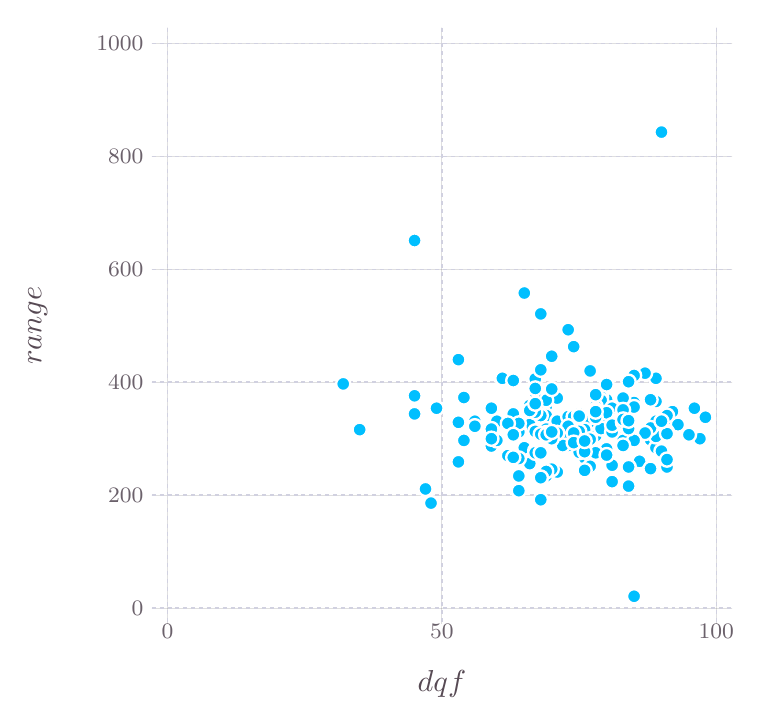
\begin{tikzpicture}[x=1mm,y=-1mm]
\definecolor{mycolor000000}{rgb}{0,0,0}
\definecolor{mycolorFFFFFF}{rgb}{1,1,1}
\definecolor{mycolor564A55}{rgb}{0.34,0.29,0.33}
\definecolor{mycolorD0D0E0}{rgb}{0.82,0.82,0.88}
\definecolor{mycolor000000}{rgb}{0,0,0}
\definecolor{mycolor6C606B}{rgb}{0.42,0.38,0.42}
\definecolor{mycolor00BFFF}{rgb}{0,0.75,1}
\begin{scope}
\begin{scope}
\draw (58.15,88.39) node [text=mycolor564A55,draw=mycolor000000,draw opacity=0,rotate around={-0: (0,1.81)},inner sep=0.0]{\fontsize{3.88mm}{4.66mm}\selectfont $\text{dqf}$};
\end{scope}
\begin{scope}
\draw (23.31,81.72) node [text=mycolor6C606B,rotate around={-0: (34.85,1.34)},inner sep=0.0]{\fontsize{2.82mm}{3.39mm}\selectfont $\text{0}$};
\draw (58.15,81.72) node [text=mycolor6C606B,rotate around={-0: (0,1.34)},inner sep=0.0]{\fontsize{2.82mm}{3.39mm}\selectfont $\text{50}$};
\draw (93,81.72) node [text=mycolor6C606B,rotate around={-0: (-34.85,1.34)},inner sep=0.0]{\fontsize{2.82mm}{3.39mm}\selectfont $\text{100}$};
\end{scope}
\begin{scope}
\clip  (21.31,5) -- (95,5) -- (95,80.72) -- (21.31,80.72);
\begin{scope}
\clip  (21.31,5) -- (95,5) -- (95,80.72) -- (21.31,80.72);
\path [fill=mycolor000000,fill opacity=0,draw=mycolor000000,draw opacity=0] (21.31,5) rectangle +(73.69,75.72);
\end{scope}
\begin{scope}
[dash pattern=on 0.5mm off 0.5mm,line width=0.2mm]
\path [fill=mycolor000000,draw=mycolorD0D0E0]  (21.31,78.72) -- (95,78.72);
\path [fill=mycolor000000,draw=mycolorD0D0E0]  (21.31,64.37) -- (95,64.37);
\path [fill=mycolor000000,draw=mycolorD0D0E0]  (21.31,50.03) -- (95,50.03);
\path [fill=mycolor000000,draw=mycolorD0D0E0]  (21.31,35.69) -- (95,35.69);
\path [fill=mycolor000000,draw=mycolorD0D0E0]  (21.31,21.34) -- (95,21.34);
\path [fill=mycolor000000,draw=mycolorD0D0E0]  (21.31,7) -- (95,7);
\end{scope}
\begin{scope}
[dash pattern=on 0.5mm off 0.5mm,line width=0.2mm]
\path [fill=mycolor000000,draw=mycolorD0D0E0]  (23.31,5) -- (23.31,80.72);
\path [fill=mycolor000000,draw=mycolorD0D0E0]  (58.15,5) -- (58.15,80.72);
\path [fill=mycolor000000,draw=mycolorD0D0E0]  (93,5) -- (93,80.72);
\end{scope}
\begin{scope}
\begin{scope}
\begin{scope}
[line width=0.3mm]
\path [fill=mycolor00BFFF,draw=mycolorFFFFFF] (82.55,77.21) circle [radius=0.9];
\path [fill=mycolor00BFFF,draw=mycolorFFFFFF] (84.64,57.34) circle [radius=0.9];
\path [fill=mycolor00BFFF,draw=mycolorFFFFFF] (56.06,63.58) circle [radius=0.9];
\path [fill=mycolor00BFFF,draw=mycolorFFFFFF] (87.42,54.98) circle [radius=0.9];
\path [fill=mycolor00BFFF,draw=mycolorFFFFFF] (85.33,49.53) circle [radius=0.9];
\path [fill=mycolor00BFFF,draw=mycolorFFFFFF] (77.67,54.55) circle [radius=0.9];
\path [fill=mycolor00BFFF,draw=mycolorFFFFFF] (65.82,49.53) circle [radius=0.9];
\path [fill=mycolor00BFFF,draw=mycolorFFFFFF] (68.61,38.7) circle [radius=0.9];
\path [fill=mycolor00BFFF,draw=mycolorFFFFFF] (70.7,64.95) circle [radius=0.9];
\path [fill=mycolor00BFFF,draw=mycolorFFFFFF] (72.79,61.43) circle [radius=0.9];
\path [fill=mycolor00BFFF,draw=mycolorFFFFFF] (83.24,60.07) circle [radius=0.9];
\path [fill=mycolor00BFFF,draw=mycolorFFFFFF] (79.76,62.65) circle [radius=0.9];
\path [fill=mycolor00BFFF,draw=mycolorFFFFFF] (90.91,57.2) circle [radius=0.9];
\path [fill=mycolor00BFFF,draw=mycolorFFFFFF] (64.43,58.13) circle [radius=0.9];
\path [fill=mycolor00BFFF,draw=mycolorFFFFFF] (83.94,48.88) circle [radius=0.9];
\path [fill=mycolor00BFFF,draw=mycolorFFFFFF] (76.27,59.64) circle [radius=0.9];
\path [fill=mycolor00BFFF,draw=mycolorFFFFFF] (85.33,58.35) circle [radius=0.9];
\path [fill=mycolor00BFFF,draw=mycolorFFFFFF] (47.7,56.05) circle [radius=0.9];
\path [fill=mycolor00BFFF,draw=mycolorFFFFFF] (80.45,55.77) circle [radius=0.9];
\path [fill=mycolor00BFFF,draw=mycolorFFFFFF] (69.3,55.41) circle [radius=0.9];
\path [fill=mycolor00BFFF,draw=mycolorFFFFFF] (75.58,56.77) circle [radius=0.9];
\path [fill=mycolor00BFFF,draw=mycolorFFFFFF] (74.88,45.51) circle [radius=0.9];
\path [fill=mycolor00BFFF,draw=mycolorFFFFFF] (67.91,56.05) circle [radius=0.9];
\path [fill=mycolor00BFFF,draw=mycolorFFFFFF] (65.12,54.98) circle [radius=0.9];
\path [fill=mycolor00BFFF,draw=mycolorFFFFFF] (86.03,18.26) circle [radius=0.9];
\path [fill=mycolor00BFFF,draw=mycolorFFFFFF] (60.94,57.42) circle [radius=0.9];
\path [fill=mycolor00BFFF,draw=mycolorFFFFFF] (68.61,58.35) circle [radius=0.9];
\path [fill=mycolor00BFFF,draw=mycolorFFFFFF] (79.06,52.25) circle [radius=0.9];
\path [fill=mycolor00BFFF,draw=mycolorFFFFFF] (72.79,52.04) circle [radius=0.9];
\path [fill=mycolor00BFFF,draw=mycolorFFFFFF] (69.3,60.36) circle [radius=0.9];
\path [fill=mycolor00BFFF,draw=mycolorFFFFFF] (76.97,60.71) circle [radius=0.9];
\path [fill=mycolor00BFFF,draw=mycolorFFFFFF] (87.42,53.76) circle [radius=0.9];
\path [fill=mycolor00BFFF,draw=mycolorFFFFFF] (71.39,53.11) circle [radius=0.9];
\path [fill=mycolor00BFFF,draw=mycolorFFFFFF] (82.55,49.17) circle [radius=0.9];
\path [fill=mycolor00BFFF,draw=mycolorFFFFFF] (72.09,55.62) circle [radius=0.9];
\path [fill=mycolor00BFFF,draw=mycolorFFFFFF] (76.97,55.12) circle [radius=0.9];
\path [fill=mycolor00BFFF,draw=mycolorFFFFFF] (75.58,55.12) circle [radius=0.9];
\path [fill=mycolor00BFFF,draw=mycolorFFFFFF] (75.58,55.98) circle [radius=0.9];
\path [fill=mycolor00BFFF,draw=mycolorFFFFFF] (79.06,53.97) circle [radius=0.9];
\path [fill=mycolor00BFFF,draw=mycolorFFFFFF] (85.33,54.98) circle [radius=0.9];
\path [fill=mycolor00BFFF,draw=mycolorFFFFFF] (76.97,55.05) circle [radius=0.9];
\path [fill=mycolor00BFFF,draw=mycolorFFFFFF] (74.18,54.12) circle [radius=0.9];
\path [fill=mycolor00BFFF,draw=mycolorFFFFFF] (64.43,55.98) circle [radius=0.9];
\path [fill=mycolor00BFFF,draw=mycolorFFFFFF] (71.39,54.26) circle [radius=0.9];
\path [fill=mycolor00BFFF,draw=mycolorFFFFFF] (67.91,61.93) circle [radius=0.9];
\path [fill=mycolor00BFFF,draw=mycolorFFFFFF] (74.18,54.26) circle [radius=0.9];
\path [fill=mycolor00BFFF,draw=mycolorFFFFFF] (65.12,57.42) circle [radius=0.9];
\path [fill=mycolor00BFFF,draw=mycolorFFFFFF] (67.91,56.34) circle [radius=0.9];
\path [fill=mycolor00BFFF,draw=mycolorFFFFFF] (74.18,56.99) circle [radius=0.9];
\path [fill=mycolor00BFFF,draw=mycolorFFFFFF] (54.67,54.05) circle [radius=0.9];
\path [fill=mycolor00BFFF,draw=mycolorFFFFFF] (69.3,52.97) circle [radius=0.9];
\path [fill=mycolor00BFFF,draw=mycolorFFFFFF] (81.15,53.97) circle [radius=0.9];
\path [fill=mycolor00BFFF,draw=mycolorFFFFFF] (74.18,57.13) circle [radius=0.9];
\path [fill=mycolor00BFFF,draw=mycolorFFFFFF] (72.09,46.73) circle [radius=0.9];
\path [fill=mycolor00BFFF,draw=mycolorFFFFFF] (91.61,54.48) circle [radius=0.9];
\path [fill=mycolor00BFFF,draw=mycolorFFFFFF] (77.67,56.84) circle [radius=0.9];
\path [fill=mycolor00BFFF,draw=mycolorFFFFFF] (71.39,55.98) circle [radius=0.9];
\path [fill=mycolor00BFFF,draw=mycolorFFFFFF] (71.39,52.32) circle [radius=0.9];
\path [fill=mycolor00BFFF,draw=mycolorFFFFFF] (70.7,54.26) circle [radius=0.9];
\path [fill=mycolor00BFFF,draw=mycolorFFFFFF] (78.36,51.89) circle [radius=0.9];
\path [fill=mycolor00BFFF,draw=mycolorFFFFFF] (85.33,52.47) circle [radius=0.9];
\path [fill=mycolor00BFFF,draw=mycolorFFFFFF] (78.36,52.32) circle [radius=0.9];
\path [fill=mycolor00BFFF,draw=mycolorFFFFFF] (86.73,56.48) circle [radius=0.9];
\path [fill=mycolor00BFFF,draw=mycolorFFFFFF] (77.67,53.11) circle [radius=0.9];
\path [fill=mycolor00BFFF,draw=mycolorFFFFFF] (74.88,56.27) circle [radius=0.9];
\path [fill=mycolor00BFFF,draw=mycolorFFFFFF] (76.27,54.98) circle [radius=0.9];
\path [fill=mycolor00BFFF,draw=mycolorFFFFFF] (74.88,54.48) circle [radius=0.9];
\path [fill=mycolor00BFFF,draw=mycolorFFFFFF] (79.06,58.49) circle [radius=0.9];
\path [fill=mycolor00BFFF,draw=mycolorFFFFFF] (82.55,52.61) circle [radius=0.9];
\path [fill=mycolor00BFFF,draw=mycolorFFFFFF] (81.85,54.12) circle [radius=0.9];
\path [fill=mycolor00BFFF,draw=mycolorFFFFFF] (78.36,54.33) circle [radius=0.9];
\path [fill=mycolor00BFFF,draw=mycolorFFFFFF] (77.67,53.54) circle [radius=0.9];
\path [fill=mycolor00BFFF,draw=mycolorFFFFFF] (81.15,57.42) circle [radius=0.9];
\path [fill=mycolor00BFFF,draw=mycolorFFFFFF] (88.12,55.41) circle [radius=0.9];
\path [fill=mycolor00BFFF,draw=mycolorFFFFFF] (90.21,53.33) circle [radius=0.9];
\path [fill=mycolor00BFFF,draw=mycolorFFFFFF] (74.88,54.26) circle [radius=0.9];
\path [fill=mycolor00BFFF,draw=mycolorFFFFFF] (78.36,55.91) circle [radius=0.9];
\path [fill=mycolor00BFFF,draw=mycolorFFFFFF] (77.67,51.61) circle [radius=0.9];
\path [fill=mycolor00BFFF,draw=mycolorFFFFFF] (84.64,52.25) circle [radius=0.9];
\path [fill=mycolor00BFFF,draw=mycolorFFFFFF] (79.76,53.33) circle [radius=0.9];
\path [fill=mycolor00BFFF,draw=mycolorFFFFFF] (79.06,53.9) circle [radius=0.9];
\path [fill=mycolor00BFFF,draw=mycolorFFFFFF] (77.67,54.48) circle [radius=0.9];
\path [fill=mycolor00BFFF,draw=mycolorFFFFFF] (85.33,56.91) circle [radius=0.9];
\path [fill=mycolor00BFFF,draw=mycolorFFFFFF] (81.15,52.04) circle [radius=0.9];
\path [fill=mycolor00BFFF,draw=mycolorFFFFFF] (81.85,49.96) circle [radius=0.9];
\path [fill=mycolor00BFFF,draw=mycolorFFFFFF] (70,51.32) circle [radius=0.9];
\path [fill=mycolor00BFFF,draw=mycolorFFFFFF] (67.21,54.05) circle [radius=0.9];
\path [fill=mycolor00BFFF,draw=mycolorFFFFFF] (70,49.6) circle [radius=0.9];
\path [fill=mycolor00BFFF,draw=mycolorFFFFFF] (72.79,54.98) circle [radius=0.9];
\path [fill=mycolor00BFFF,draw=mycolorFFFFFF] (77.67,53.76) circle [radius=0.9];
\path [fill=mycolor00BFFF,draw=mycolorFFFFFF] (81.15,53.97) circle [radius=0.9];
\path [fill=mycolor00BFFF,draw=mycolorFFFFFF] (74.18,54.4) circle [radius=0.9];
\path [fill=mycolor00BFFF,draw=mycolorFFFFFF] (75.58,54.26) circle [radius=0.9];
\path [fill=mycolor00BFFF,draw=mycolorFFFFFF] (91.61,54.48) circle [radius=0.9];
\path [fill=mycolor00BFFF,draw=mycolorFFFFFF] (79.06,50.32) circle [radius=0.9];
\path [fill=mycolor00BFFF,draw=mycolorFFFFFF] (76.27,56.05) circle [radius=0.9];
\path [fill=mycolor00BFFF,draw=mycolorFFFFFF] (81.85,54.76) circle [radius=0.9];
\path [fill=mycolor00BFFF,draw=mycolorFFFFFF] (71.39,56.48) circle [radius=0.9];
\path [fill=mycolor00BFFF,draw=mycolorFFFFFF] (62.33,54.98) circle [radius=0.9];
\path [fill=mycolor00BFFF,draw=mycolorFFFFFF] (54.67,51.75) circle [radius=0.9];
\path [fill=mycolor00BFFF,draw=mycolorFFFFFF] (45.61,50.24) circle [radius=0.9];
\path [fill=mycolor00BFFF,draw=mycolorFFFFFF] (75.58,56.27) circle [radius=0.9];
\path [fill=mycolor00BFFF,draw=mycolorFFFFFF] (60.24,55.12) circle [radius=0.9];
\path [fill=mycolor00BFFF,draw=mycolorFFFFFF] (56.76,65.38) circle [radius=0.9];
\path [fill=mycolor00BFFF,draw=mycolorFFFFFF] (74.18,58.06) circle [radius=0.9];
\path [fill=mycolor00BFFF,draw=mycolorFFFFFF] (70.7,48.45) circle [radius=0.9];
\path [fill=mycolor00BFFF,draw=mycolorFFFFFF] (76.27,61.22) circle [radius=0.9];
\path [fill=mycolor00BFFF,draw=mycolorFFFFFF] (67.91,55.26) circle [radius=0.9];
\path [fill=mycolor00BFFF,draw=mycolorFFFFFF] (82.55,53.18) circle [radius=0.9];
\path [fill=mycolor00BFFF,draw=mycolorFFFFFF] (60.94,51.97) circle [radius=0.9];
\path [fill=mycolor00BFFF,draw=mycolorFFFFFF] (77.67,58.99) circle [radius=0.9];
\path [fill=mycolor00BFFF,draw=mycolorFFFFFF] (75.58,58.92) circle [radius=0.9];
\path [fill=mycolor00BFFF,draw=mycolorFFFFFF] (72.09,50.89) circle [radius=0.9];
\path [fill=mycolor00BFFF,draw=mycolorFFFFFF] (70.7,41.35) circle [radius=0.9];
\path [fill=mycolor00BFFF,draw=mycolorFFFFFF] (70.7,41.35) circle [radius=0.9];
\path [fill=mycolor00BFFF,draw=mycolorFFFFFF] (86.73,56.34) circle [radius=0.9];
\path [fill=mycolor00BFFF,draw=mycolorFFFFFF] (70,53.83) circle [radius=0.9];
\path [fill=mycolor00BFFF,draw=mycolorFFFFFF] (86.73,54.26) circle [radius=0.9];
\path [fill=mycolor00BFFF,draw=mycolorFFFFFF] (74.18,43.36) circle [radius=0.9];
\path [fill=mycolor00BFFF,draw=mycolorFFFFFF] (86.73,60.79) circle [radius=0.9];
\path [fill=mycolor00BFFF,draw=mycolorFFFFFF] (84.64,61) circle [radius=0.9];
\path [fill=mycolor00BFFF,draw=mycolorFFFFFF] (84.64,55.84) circle [radius=0.9];
\path [fill=mycolor00BFFF,draw=mycolorFFFFFF] (66.52,59.42) circle [radius=0.9];
\path [fill=mycolor00BFFF,draw=mycolorFFFFFF] (74.88,54.4) circle [radius=0.9];
\path [fill=mycolor00BFFF,draw=mycolorFFFFFF] (73.49,58.06) circle [radius=0.9];
\path [fill=mycolor00BFFF,draw=mycolorFFFFFF] (86.73,56.56) circle [radius=0.9];
\path [fill=mycolor00BFFF,draw=mycolorFFFFFF] (74.18,55.62) circle [radius=0.9];
\path [fill=mycolor00BFFF,draw=mycolorFFFFFF] (76.27,58.85) circle [radius=0.9];
\path [fill=mycolor00BFFF,draw=mycolorFFFFFF] (76.97,48.59) circle [radius=0.9];
\path [fill=mycolor00BFFF,draw=mycolorFFFFFF] (69.3,53.61) circle [radius=0.9];
\path [fill=mycolor00BFFF,draw=mycolorFFFFFF] (71.39,61.93) circle [radius=0.9];
\path [fill=mycolor00BFFF,draw=mycolorFFFFFF] (74.88,56.48) circle [radius=0.9];
\path [fill=mycolor00BFFF,draw=mycolorFFFFFF] (70,56.27) circle [radius=0.9];
\path [fill=mycolor00BFFF,draw=mycolorFFFFFF] (86.03,54.98) circle [radius=0.9];
\path [fill=mycolor00BFFF,draw=mycolorFFFFFF] (83.94,56.48) circle [radius=0.9];
\path [fill=mycolor00BFFF,draw=mycolorFFFFFF] (76.97,57.27) circle [radius=0.9];
\path [fill=mycolor00BFFF,draw=mycolorFFFFFF] (82.55,57.42) circle [radius=0.9];
\path [fill=mycolor00BFFF,draw=mycolorFFFFFF] (81.15,55.41) circle [radius=0.9];
\path [fill=mycolor00BFFF,draw=mycolorFFFFFF] (81.15,58.06) circle [radius=0.9];
\path [fill=mycolor00BFFF,draw=mycolorFFFFFF] (67.91,59.71) circle [radius=0.9];
\path [fill=mycolor00BFFF,draw=mycolorFFFFFF] (66.52,59.35) circle [radius=0.9];
\path [fill=mycolor00BFFF,draw=mycolorFFFFFF] (79.76,60.57) circle [radius=0.9];
\path [fill=mycolor00BFFF,draw=mycolorFFFFFF] (74.88,57.7) circle [radius=0.9];
\path [fill=mycolor00BFFF,draw=mycolorFFFFFF] (81.15,53.54) circle [radius=0.9];
\path [fill=mycolor00BFFF,draw=mycolorFFFFFF] (70.7,56.63) circle [radius=0.9];
\path [fill=mycolor00BFFF,draw=mycolorFFFFFF] (79.76,56.34) circle [radius=0.9];
\path [fill=mycolor00BFFF,draw=mycolorFFFFFF] (60.24,60.14) circle [radius=0.9];
\path [fill=mycolor00BFFF,draw=mycolorFFFFFF] (72.09,61.07) circle [radius=0.9];
\path [fill=mycolor00BFFF,draw=mycolorFFFFFF] (72.79,56.48) circle [radius=0.9];
\path [fill=mycolor00BFFF,draw=mycolorFFFFFF] (72.79,56.48) circle [radius=0.9];
\path [fill=mycolor00BFFF,draw=mycolorFFFFFF] (72.09,56.48) circle [radius=0.9];
\path [fill=mycolor00BFFF,draw=mycolorFFFFFF] (72.09,57.2) circle [radius=0.9];
\path [fill=mycolor00BFFF,draw=mycolorFFFFFF] (70,58.71) circle [radius=0.9];
\path [fill=mycolor00BFFF,draw=mycolorFFFFFF] (66.52,55.26) circle [radius=0.9];
\path [fill=mycolor00BFFF,draw=mycolorFFFFFF] (70,52.75) circle [radius=0.9];
\path [fill=mycolor00BFFF,draw=mycolorFFFFFF] (75.58,54.05) circle [radius=0.9];
\path [fill=mycolor00BFFF,draw=mycolorFFFFFF] (71.39,56.7) circle [radius=0.9];
\path [fill=mycolor00BFFF,draw=mycolorFFFFFF] (64.43,57.2) circle [radius=0.9];
\path [fill=mycolor00BFFF,draw=mycolorFFFFFF] (79.76,55.48) circle [radius=0.9];
\path [fill=mycolor00BFFF,draw=mycolorFFFFFF] (86.03,58.78) circle [radius=0.9];
\path [fill=mycolor00BFFF,draw=mycolorFFFFFF] (70,58.99) circle [radius=0.9];
\path [fill=mycolor00BFFF,draw=mycolorFFFFFF] (81.15,55.12) circle [radius=0.9];
\path [fill=mycolor00BFFF,draw=mycolorFFFFFF] (81.15,55.12) circle [radius=0.9];
\path [fill=mycolor00BFFF,draw=mycolorFFFFFF] (71.39,61.36) circle [radius=0.9];
\path [fill=mycolor00BFFF,draw=mycolorFFFFFF] (89.52,56.7) circle [radius=0.9];
\path [fill=mycolor00BFFF,draw=mycolorFFFFFF] (81.85,55.91) circle [radius=0.9];
\path [fill=mycolor00BFFF,draw=mycolorFFFFFF] (67.21,49.81) circle [radius=0.9];
\path [fill=mycolor00BFFF,draw=mycolorFFFFFF] (67.21,59.57) circle [radius=0.9];
\path [fill=mycolor00BFFF,draw=mycolorFFFFFF] (81.15,54.76) circle [radius=0.9];
\path [fill=mycolor00BFFF,draw=mycolorFFFFFF] (70.7,62.15) circle [radius=0.9];
\path [fill=mycolor00BFFF,draw=mycolorFFFFFF] (70.7,62.15) circle [radius=0.9];
\path [fill=mycolor00BFFF,draw=mycolorFFFFFF] (67.91,63.8) circle [radius=0.9];
\path [fill=mycolor00BFFF,draw=mycolorFFFFFF] (79.06,59.28) circle [radius=0.9];
\path [fill=mycolor00BFFF,draw=mycolorFFFFFF] (67.21,56.7) circle [radius=0.9];
\path [fill=mycolor00BFFF,draw=mycolorFFFFFF] (81.85,60.79) circle [radius=0.9];
\path [fill=mycolor00BFFF,draw=mycolorFFFFFF] (81.85,60.79) circle [radius=0.9];
\path [fill=mycolor00BFFF,draw=mycolorFFFFFF] (64.43,53.33) circle [radius=0.9];
\path [fill=mycolor00BFFF,draw=mycolorFFFFFF] (76.27,57.49) circle [radius=0.9];
\path [fill=mycolor00BFFF,draw=mycolorFFFFFF] (70,50.82) circle [radius=0.9];
\path [fill=mycolor00BFFF,draw=mycolorFFFFFF] (70.7,58.99) circle [radius=0.9];
\path [fill=mycolor00BFFF,draw=mycolorFFFFFF] (57.46,53.33) circle [radius=0.9];
\path [fill=mycolor00BFFF,draw=mycolorFFFFFF] (86.73,59.85) circle [radius=0.9];
\path [fill=mycolor00BFFF,draw=mycolorFFFFFF] (81.85,63.22) circle [radius=0.9];
\path [fill=mycolor00BFFF,draw=mycolorFFFFFF] (60.24,47.16) circle [radius=0.9];
\path [fill=mycolor00BFFF,draw=mycolorFFFFFF] (72.09,56.34) circle [radius=0.9];
\path [fill=mycolor00BFFF,draw=mycolorFFFFFF] (81.85,54.91) circle [radius=0.9];
\path [fill=mycolor00BFFF,draw=mycolorFFFFFF] (62.33,55.62) circle [radius=0.9];
\path [fill=mycolor00BFFF,draw=mycolorFFFFFF] (54.67,32.03) circle [radius=0.9];
\path [fill=mycolor00BFFF,draw=mycolorFFFFFF] (75.58,54.33) circle [radius=0.9];
\end{scope}
\end{scope}
\end{scope}
\end{scope}
\begin{scope}
\draw (20.31,78.72) node [text=mycolor6C606B,rotate around={-0: (-3.35,-35.86)},left,inner sep=0.0]{\fontsize{2.82mm}{3.39mm}\selectfont $\text{0}$};
\draw (20.31,64.37) node [text=mycolor6C606B,rotate around={-0: (-3.35,-21.51)},left,inner sep=0.0]{\fontsize{2.82mm}{3.39mm}\selectfont $\text{200}$};
\draw (20.31,50.03) node [text=mycolor6C606B,rotate around={-0: (-3.35,-7.17)},left,inner sep=0.0]{\fontsize{2.82mm}{3.39mm}\selectfont $\text{400}$};
\draw (20.31,35.69) node [text=mycolor6C606B,rotate around={-0: (-3.35,7.17)},left,inner sep=0.0]{\fontsize{2.82mm}{3.39mm}\selectfont $\text{600}$};
\draw (20.31,21.34) node [text=mycolor6C606B,rotate around={-0: (-3.35,21.51)},left,inner sep=0.0]{\fontsize{2.82mm}{3.39mm}\selectfont $\text{800}$};
\draw (20.31,7) node [text=mycolor6C606B,rotate around={-0: (-3.35,35.86)},left,inner sep=0.0]{\fontsize{2.82mm}{3.39mm}\selectfont $\text{1000}$};
\end{scope}
\begin{scope}
\draw (8.81,40.86) node [text=mycolor564A55,draw=mycolor000000,draw opacity=0,rotate around={90: (0,2)},inner sep=0.0]{\fontsize{3.88mm}{4.66mm}\selectfont $\text{range}$};
\end{scope}
\end{scope}
\end{tikzpicture}

	\caption{100 values measured at 2m distance}
	\label{2m}
\end{figure}

\subsection{Antenna Orientation}
\todo{ (diversity, no diversity) * (parallel, perpendicular) }


\subsection{Influence of Distance}

\subsection{Orientation of Devices}


\subsection{Moving Nodes}

\subsection{Ranging on FINken Robots}

\section{Properties of a Distance Function}
The ranging sensor on the FINken robot shall be used to provide a distance between two quadcopters, similar to a distance measure used in swarm intelligence algorithms.
In the pure mathematical sense a distance function has to fullfill certian properties.

If $f(x, y)$ is a distance function it has to have the following properties.
\begin{eqnarray}
f(x, y) \ge 0 \\
f(x, y) = 0 \iff x = y \\ 
f(x, y) = f(y, x) \\ 
f(x, z) \le f(x, y) + f(y, z)
\end{eqnarray}

Of course the value measured by any real sensor will not completly accomplish to satisfy those conditions.
For use in swarm robotics it is therefore very interesting to know in which way the range values break the pattern of a mathematical distance function.

\subsection{Non-negativity and Coincidence}

\subsection{Symmetry}

\subsection{Triangle Inequality}



\section{Conclusion}
